% !TEX root = main.tex
% \documentclass{tufte-book}%[a4paper,twoside]
% See https://github.com/Tufte-LaTeX/tufte-latex/blob/master/sample-book.tex for details

% --- AMAZON BEGIN ---
% WITHOUT BLEED
% US Trade => 6x9
\documentclass[paper=6in:9in,pagesize=pdftex,
               headinclude=on,footinclude=on,12pt]{scrbook}
%
% Paper width
% W = 6in
% Paper height
% H = 9in
% Paper gutter
% BCOR = 0.5in
% Margin (0.5in imposed on lulu, recommended on createspace)
% m = 0.5in
% Text height
% h = H - 2m = 8in
% Text width
% w = W - 2m - BCOR = 4.5in
\areaset[0.50in]{4.5in}{8in}
% --- AMAZON END ---

\title{21 Lessons}
\subtitle{What I've Learned from Falling Down the Bitcoin Rabbit Hole }
\author{Gigi}

% Packages
\usepackage{lipsum}
\usepackage{booktabs}
\usepackage{graphicx}
\setkeys{Gin}{width=\linewidth,totalheight=\textheight,keepaspectratio}
\graphicspath{{graphics/}}

%%
% For Quotes
\usepackage{csquotes}
\renewcommand\mkbegdispquote[2]{\makebox[0pt][r]{\textquotedblleft\,}}
\renewcommand\mkenddispquote[2]{\,\textquotedblright#2}

%%
% Just some sample text
\usepackage{lipsum}

%%
% For nicely typeset tabular material
\usepackage{booktabs}

%%
% Bibliography stuff: Biber, BibTex, BibLatex
%\usepackage[autostyle]{csquotes}
% \usepackage[
    % backend=biber,
    % style=authoryear-icomp,
    % sortlocale=de_DE,
    % natbib=true,
    % url=false,
    % doi=true,
    % eprint=false
% ]{biblatex}
% \usepackage[backend=biber]{biblatex}
\usepackage{natbib}
\bibliographystyle{abbrvnat}

%%
% Hyperlinks
\usepackage{hyperref}

%%
% For graphics / images
\usepackage{graphicx}
\setkeys{Gin}{width=\linewidth,totalheight=\textheight,keepaspectratio}
\graphicspath{{graphics/}}

% The fancyvrb package lets us customize the formatting of verbatim
% environments.  We use a slightly smaller font.
\usepackage{fancyvrb}
\fvset{fontsize=\normalsize}

%%
% Prints argument within hanging parentheses (i.e., parentheses that take
% up no horizontal space).  Useful in tabular environments.
\newcommand{\hangp}[1]{\makebox[0pt][r]{(}#1\makebox[0pt][l]{)}}

%%
% Prints an asterisk that takes up no horizontal space.
% Useful in tabular environments.
\newcommand{\hangstar}{\makebox[0pt][l]{*}}

%%
% Prints a trailing space in a smart way.
\usepackage{xspace}

% Prints the month name (e.g., January) and the year (e.g., 2008)
\newcommand{\monthyear}{%
  \ifcase\month\or January\or February\or March\or April\or May\or June\or
  July\or August\or September\or October\or November\or
  December\fi\space\number\year
}


% Prints an epigraph and speaker in sans serif, all-caps type.
\newcommand{\openepigraph}[2]{%
  %\sffamily\fontsize{14}{16}\selectfont
  \begin{fullwidth}
  \sffamily\large
  \begin{doublespace}
  \noindent\allcaps{#1}\\% epigraph
  \noindent\allcaps{#2}% author
  \end{doublespace}
  \end{fullwidth}
}

% Inserts a blank page
\newcommand{\blankpage}{\newpage\hbox{}\thispagestyle{empty}\newpage}

\usepackage{units}

% Typesets the font size, leading, and measure in the form of 10/12x26 pc.
\newcommand{\measure}[3]{#1/#2$\times$\unit[#3]{pc}}

% Macros for typesetting the documentation
\newcommand{\hlred}[1]{\textcolor{Maroon}{#1}}% prints in red
\newcommand{\hangleft}[1]{\makebox[0pt][r]{#1}}
\newcommand{\hairsp}{\hspace{1pt}}% hair space
\newcommand{\hquad}{\hskip0.5em\relax}% half quad space
\newcommand{\TODO}{\textcolor{red}{\bf TODO!}\xspace}
\newcommand{\na}{\quad--}% used in tables for N/A cells
\providecommand{\XeLaTeX}{X\lower.5ex\hbox{\kern-0.15em\reflectbox{E}}\kern-0.1em\LaTeX}
\newcommand{\tXeLaTeX}{\XeLaTeX\index{XeLaTeX@\protect\XeLaTeX}}
% \index{\texttt{\textbackslash xyz}@\hangleft{\texttt{\textbackslash}}\texttt{xyz}}
\newcommand{\tuftebs}{\symbol{'134}}% a backslash in tt type in OT1/T1
\newcommand{\doccmdnoindex}[2][]{\texttt{\tuftebs#2}}% command name -- adds backslash automatically (and doesn't add cmd to the index)
\newcommand{\doccmddef}[2][]{%
  \hlred{\texttt{\tuftebs#2}}\label{cmd:#2}%
  \ifthenelse{\isempty{#1}}%
    {% add the command to the index
      \index{#2 command@\protect\hangleft{\texttt{\tuftebs}}\texttt{#2}}% command name
    }%
    {% add the command and package to the index
      \index{#2 command@\protect\hangleft{\texttt{\tuftebs}}\texttt{#2} (\texttt{#1} package)}% command name
      \index{#1 package@\texttt{#1} package}\index{packages!#1@\texttt{#1}}% package name
    }%
}% command name -- adds backslash automatically
\newcommand{\doccmd}[2][]{%
  \texttt{\tuftebs#2}%
  \ifthenelse{\isempty{#1}}%
    {% add the command to the index
      \index{#2 command@\protect\hangleft{\texttt{\tuftebs}}\texttt{#2}}% command name
    }%
    {% add the command and package to the index
      \index{#2 command@\protect\hangleft{\texttt{\tuftebs}}\texttt{#2} (\texttt{#1} package)}% command name
      \index{#1 package@\texttt{#1} package}\index{packages!#1@\texttt{#1}}% package name
    }%
}% command name -- adds backslash automatically
\newcommand{\docopt}[1]{\ensuremath{\langle}\textrm{\textit{#1}}\ensuremath{\rangle}}% optional command argument
\newcommand{\docarg}[1]{\textrm{\textit{#1}}}% (required) command argument
\newenvironment{docspec}{\begin{quotation}\ttfamily\parskip0pt\parindent0pt\ignorespaces}{\end{quotation}}% command specification environment
\newcommand{\docenv}[1]{\texttt{#1}\index{#1 environment@\texttt{#1} environment}\index{environments!#1@\texttt{#1}}}% environment name
\newcommand{\docenvdef}[1]{\hlred{\texttt{#1}}\label{env:#1}\index{#1 environment@\texttt{#1} environment}\index{environments!#1@\texttt{#1}}}% environment name
\newcommand{\docpkg}[1]{\texttt{#1}\index{#1 package@\texttt{#1} package}\index{packages!#1@\texttt{#1}}}% package name
\newcommand{\doccls}[1]{\texttt{#1}}% document class name
\newcommand{\docclsopt}[1]{\texttt{#1}\index{#1 class option@\texttt{#1} class option}\index{class options!#1@\texttt{#1}}}% document class option name
\newcommand{\docclsoptdef}[1]{\hlred{\texttt{#1}}\label{clsopt:#1}\index{#1 class option@\texttt{#1} class option}\index{class options!#1@\texttt{#1}}}% document class option name defined
\newcommand{\docmsg}[2]{\bigskip\begin{fullwidth}\noindent\ttfamily#1\end{fullwidth}\medskip\par\noindent#2}
\newcommand{\docfilehook}[2]{\texttt{#1}\index{file hooks!#2}\index{#1@\texttt{#1}}}
\newcommand{\doccounter}[1]{\texttt{#1}\index{#1 counter@\texttt{#1} counter}}

% Generates the index
\usepackage{makeidx}
\makeindex

%%
% Chapter/Lesson Quotes
\makeatletter
\renewcommand{\@chapapp}{}% Not necessary...
\newenvironment{chapquote}[2][4em]
  {\setlength{\@tempdima}{#1}%
   \def\chapquote@author{#2}%
   \parshape 1 \@tempdima \dimexpr\textwidth-2\@tempdima\relax%
   \itshape}
  {\par\normalfont\hfill--\ \chapquote@author\hspace*{\@tempdima}\par\bigskip}
\makeatother

\begin{document}

\frontmatter

\maketitle

\cleardoublepage


%%
% Start the main matter (normal chapters)
\mainmatter

\chapter*{Einleitung}
\label{ch:introduction}

\begin{chapquote}{Lewis Carroll, \textit{Alice im Wunderland}}
\enquote{Aber ich möchte nicht unter verrückte Leute geraten,} bemerkte Alice.
\enquote{Oh, da kommst du nicht drum herum,} sagte die Katze: \enquote{Wir sind
hier alle verrückt. Ich bin verrückt. Du bist verrückt.} \enquote{Woher weißt
du, daß ich verrückt bin?} sagte Alice. \enquote{du mußt es sein,} sagte die
Katze, \enquote{sonst wärst du nicht hergekommen.}
\end{chapquote}

Im Oktober 2018 stellte Arjun Balaji die harmlose Frage: \textit{Was hast du von
Bitcoin gelernt?} Nachdem ich versucht hatte, diese Frage in einem kurzen Tweet
zu beantworten, und kläglich scheiterte, wurde mir klar, dass die Dinge, die ich
gelernt habe viel zu zahlreich sind, um sie schnell oder überhaupt zu
beantworten.

Die Dinge, die ich gelernt habe, sind offensichtlich auf Bitcoin bezogen – oder
stehen zumindest im Zusammenhang damit. Obwohl einige der inneren Funktionen von
Bitcoin am Rande erklärt werden, sind die folgenden Lektionen keine Erklärung
dafür, wie Bitcoin funktioniert oder was es ist. Sie könnten jedoch helfen,
einige der Dinge zu erkunden, die Bitcoin berührt: philosophische Fragen,
wirtschaftliche Gegebenheiten und technologische Innovationen.

\begin{center}
  
\includegraphics[width=7cm]{assets/images/the-tweet.png}
\end{center}

Die \textit{21 Lektionen} sind in Siebener-Bündel gegliedert, was letztendlich
zu drei Teilen führt. Jeder Teil betrachtet Bitcoin durch eine
unterschiedliche Linse und zeigt, welche Erkenntnisse daraus gezogen werden
können, wenn man dieses seltsame Netzwerk aus einem anderen Blickwinkel
betrachtet.

\paragraph{\hyperref[ch:philosophy]{Teil I}} untersucht die philosophischen
Lehren von Bitcoin. Das Zusammenspiel von Unveränderlichkeit und Veränderung,
das Konzept der wahren Knappheit, Bitcoins unbefleckte Empfängnis, das Problem
der Identität, der Widerspruch von Replikation und Lokalität, die Macht der freien
Meinungsäußerung und die Grenzen des Wissens.

\paragraph{\hyperref[ch:economics]{Teil II}} untersucht die wirtschaftlichen
Lehren von Bitcoin. Lektionen über finanzielle Unwissenheit, Inflation, Wert,
Geld und die Geschichte des Geldes, Mindestreserve-Bankensystem und wie Bitcoin
auf raffinierte und kuriose Weise wieder gesundes bzw. solides Geld auf den
Markt bringt.

\paragraph{\hyperref[ch:technology]{Teil III}} untersucht einige der Lehren, die
aus der Auseinandersetzung mit der Technologie von Bitcoin hervorgegangen sind.
Warum Stärke in Zahlen zu finden ist, was Vertrauen bedeutet, warum das
Messen von Zeit arbeitsintensiv ist, warum behutsames Fortbewegen ein Feature
und kein Bug ist, was die Erschaffung von Bitcoin uns über die Privatsphäre
vermitteln kann, warum Cypherpunks Code schreiben (und nicht Gesetze) und welche
Metaphern nützlich sein könnten, um die Zukunft von Bitcoin zu erforschen.

~

Jede Lektion enthält mehrere Zitate und Links im gesamten Text. Wenn du tiefer
in die Materie eintauchen möchtest, findest du Links zu den wichtigsten
Materialien in den Fußnoten und in den Quellenangaben am Ende des Buches.

Auch wenn einige Vorkenntnisse über Bitcoin von Vorteil sind, hoffe ich, dass
diese Lektionen von jedem interessierten Leser verinnerlicht werden können.
Während einige sich aufeinander beziehen, sollte jede Lektion für sich allein
stehen und unabhängig voneinander gelesen werden können. Ich habe mein Bestes
getan, um mich vor Fachjargon zu scheuen, auch wenn einige domänenspezifische
Vokabeln unvermeidlich sind.

Ich hoffe, dass mein Schreiben anderen als Inspiration dient etwas tiefer
zu graben und einige der weitgreiferenden Fragen zu untersuchen welche Bitcoin
aufwirft. Meine eigene Inspiration kam von einer Vielzahl von Autoren, Bloggern,
und anderen kreativen Köpfen aus dem Internet, welchen ich ewig dankbar bin.

Zu guter Letzt: Mir geht es nicht darum dich, lieber Leser, von irgendetwas zu
überzeugen. Mein Ziel ist es dich zum Nachdenken zu bringen und dir zu zeigen,
dass hinter Bitcoin mehr steckt als man denkt. Ich kann dir gar nicht sagen,
was Bitcoin ist oder was Bitcoin dir beibringen wird. Das musst du selbst
herausfinden.

\begin{quotation}\begin{samepage}
\enquote{Danach gibt es kein Zurück mehr. Du nimmst die blaue Pille --- die
Geschichte endet hier, du wachst in deinem Bett auf und glaubst, was du glauben
willst. Du nimmst die rote Pille\footnote{die \textit{orange} Pille} --- du
bleibst im Wunderland, und ich zeige dir, wie weit der Kaninchenbau reicht.}
\begin{flushright} -- Morpheus
\end{flushright}\end{samepage}\end{quotation}

\begin{figure}
  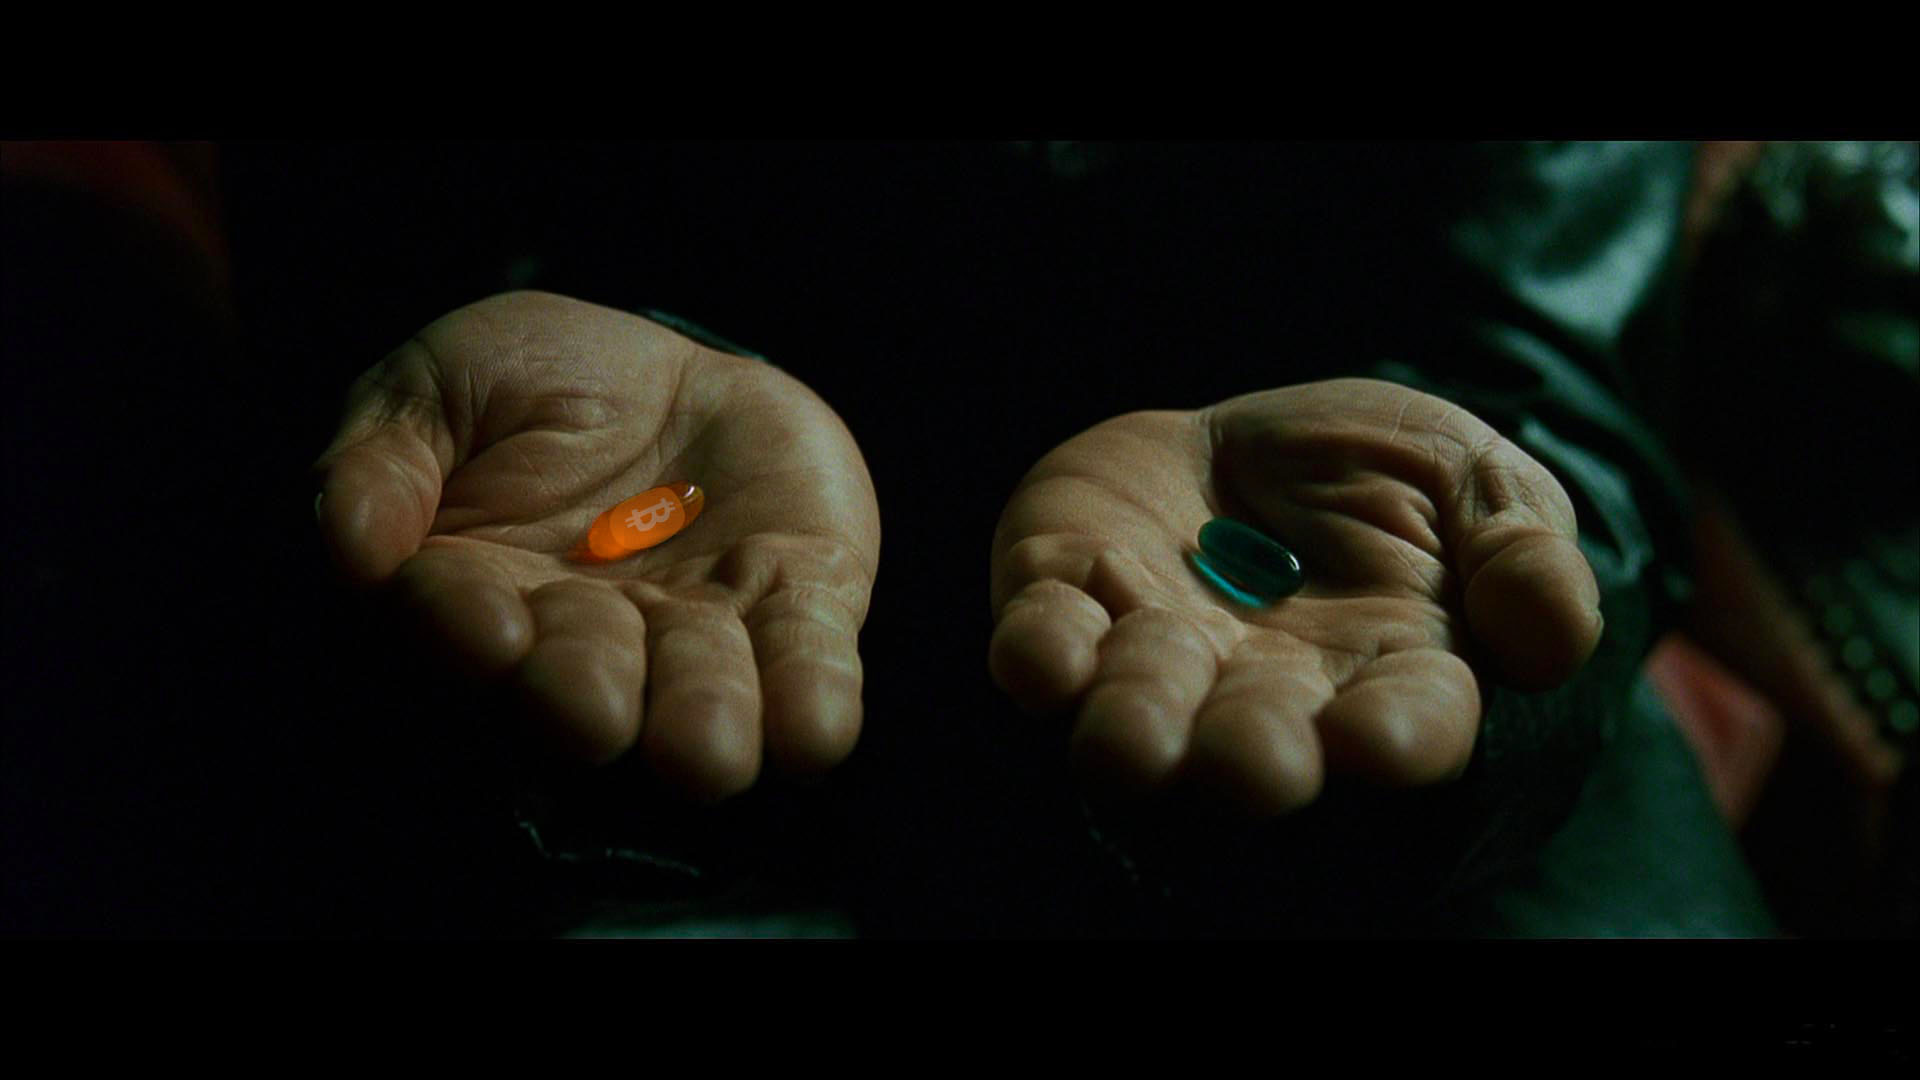
\includegraphics[width=\textwidth]{assets/images/bitcoin-orange-pill.jpg}
  \caption*{Bedenke! Alles, was ich dir anbiete, ist die Wahrheit. Nicht mehr.}
  \label{fig:bitcoin-orange-pill}
\end{figure}

%
% [Morpheus]: https://en.wikipedia.org/wiki/Red_pill_and_blue_pill#The_Matrix_(1999)
% [this question]: https://twitter.com/arjunblj/status/1050073234719293440
%
% <!-- Internal -->
% [chapter1]: {{ 'bitcoin/lessons/ch1-00-philosophy' | absolute_url }}
% [chapter2]: {{ 'bitcoin/lessons/ch2-00-economics' | absolute_url }}
% [chapter3]: {{ 'bitcoin/lessons/ch3-00-technology' | absolute_url }}
%
% <!-- Wikipedia -->
% [alice]: https://en.wikipedia.org/wiki/Alice%27s_Adventures_in_Wonderland
% [carroll]: https://en.wikipedia.org/wiki/Lewis_Carroll

\part{Philosophy}
\label{ch:philosophy}
\chapter*{Philosophy}

\begin{chapquote}{Lewis Carroll, \textit{Alice in Wonderland}}
The mouse looked at her rather inquisitively, and seemed to her to wink with one
of its little eyes, but it said nothing.
\end{chapquote}

Looking at Bitcoin superficially, one might conclude that it is slow, wasteful,
unnecessarily redundant, and overly paranoid. Looking at Bitcoin inquisitively,
one might find out that things are not as they seem at first glance.

Bitcoin has a way of taking your assumptions and turning them on their heads.
After a while, just when you were about to get comfortable again, Bitcoin will
smash through the wall like a bull in a china shop and shatter your assumptions
once more.

\begin{figure}
  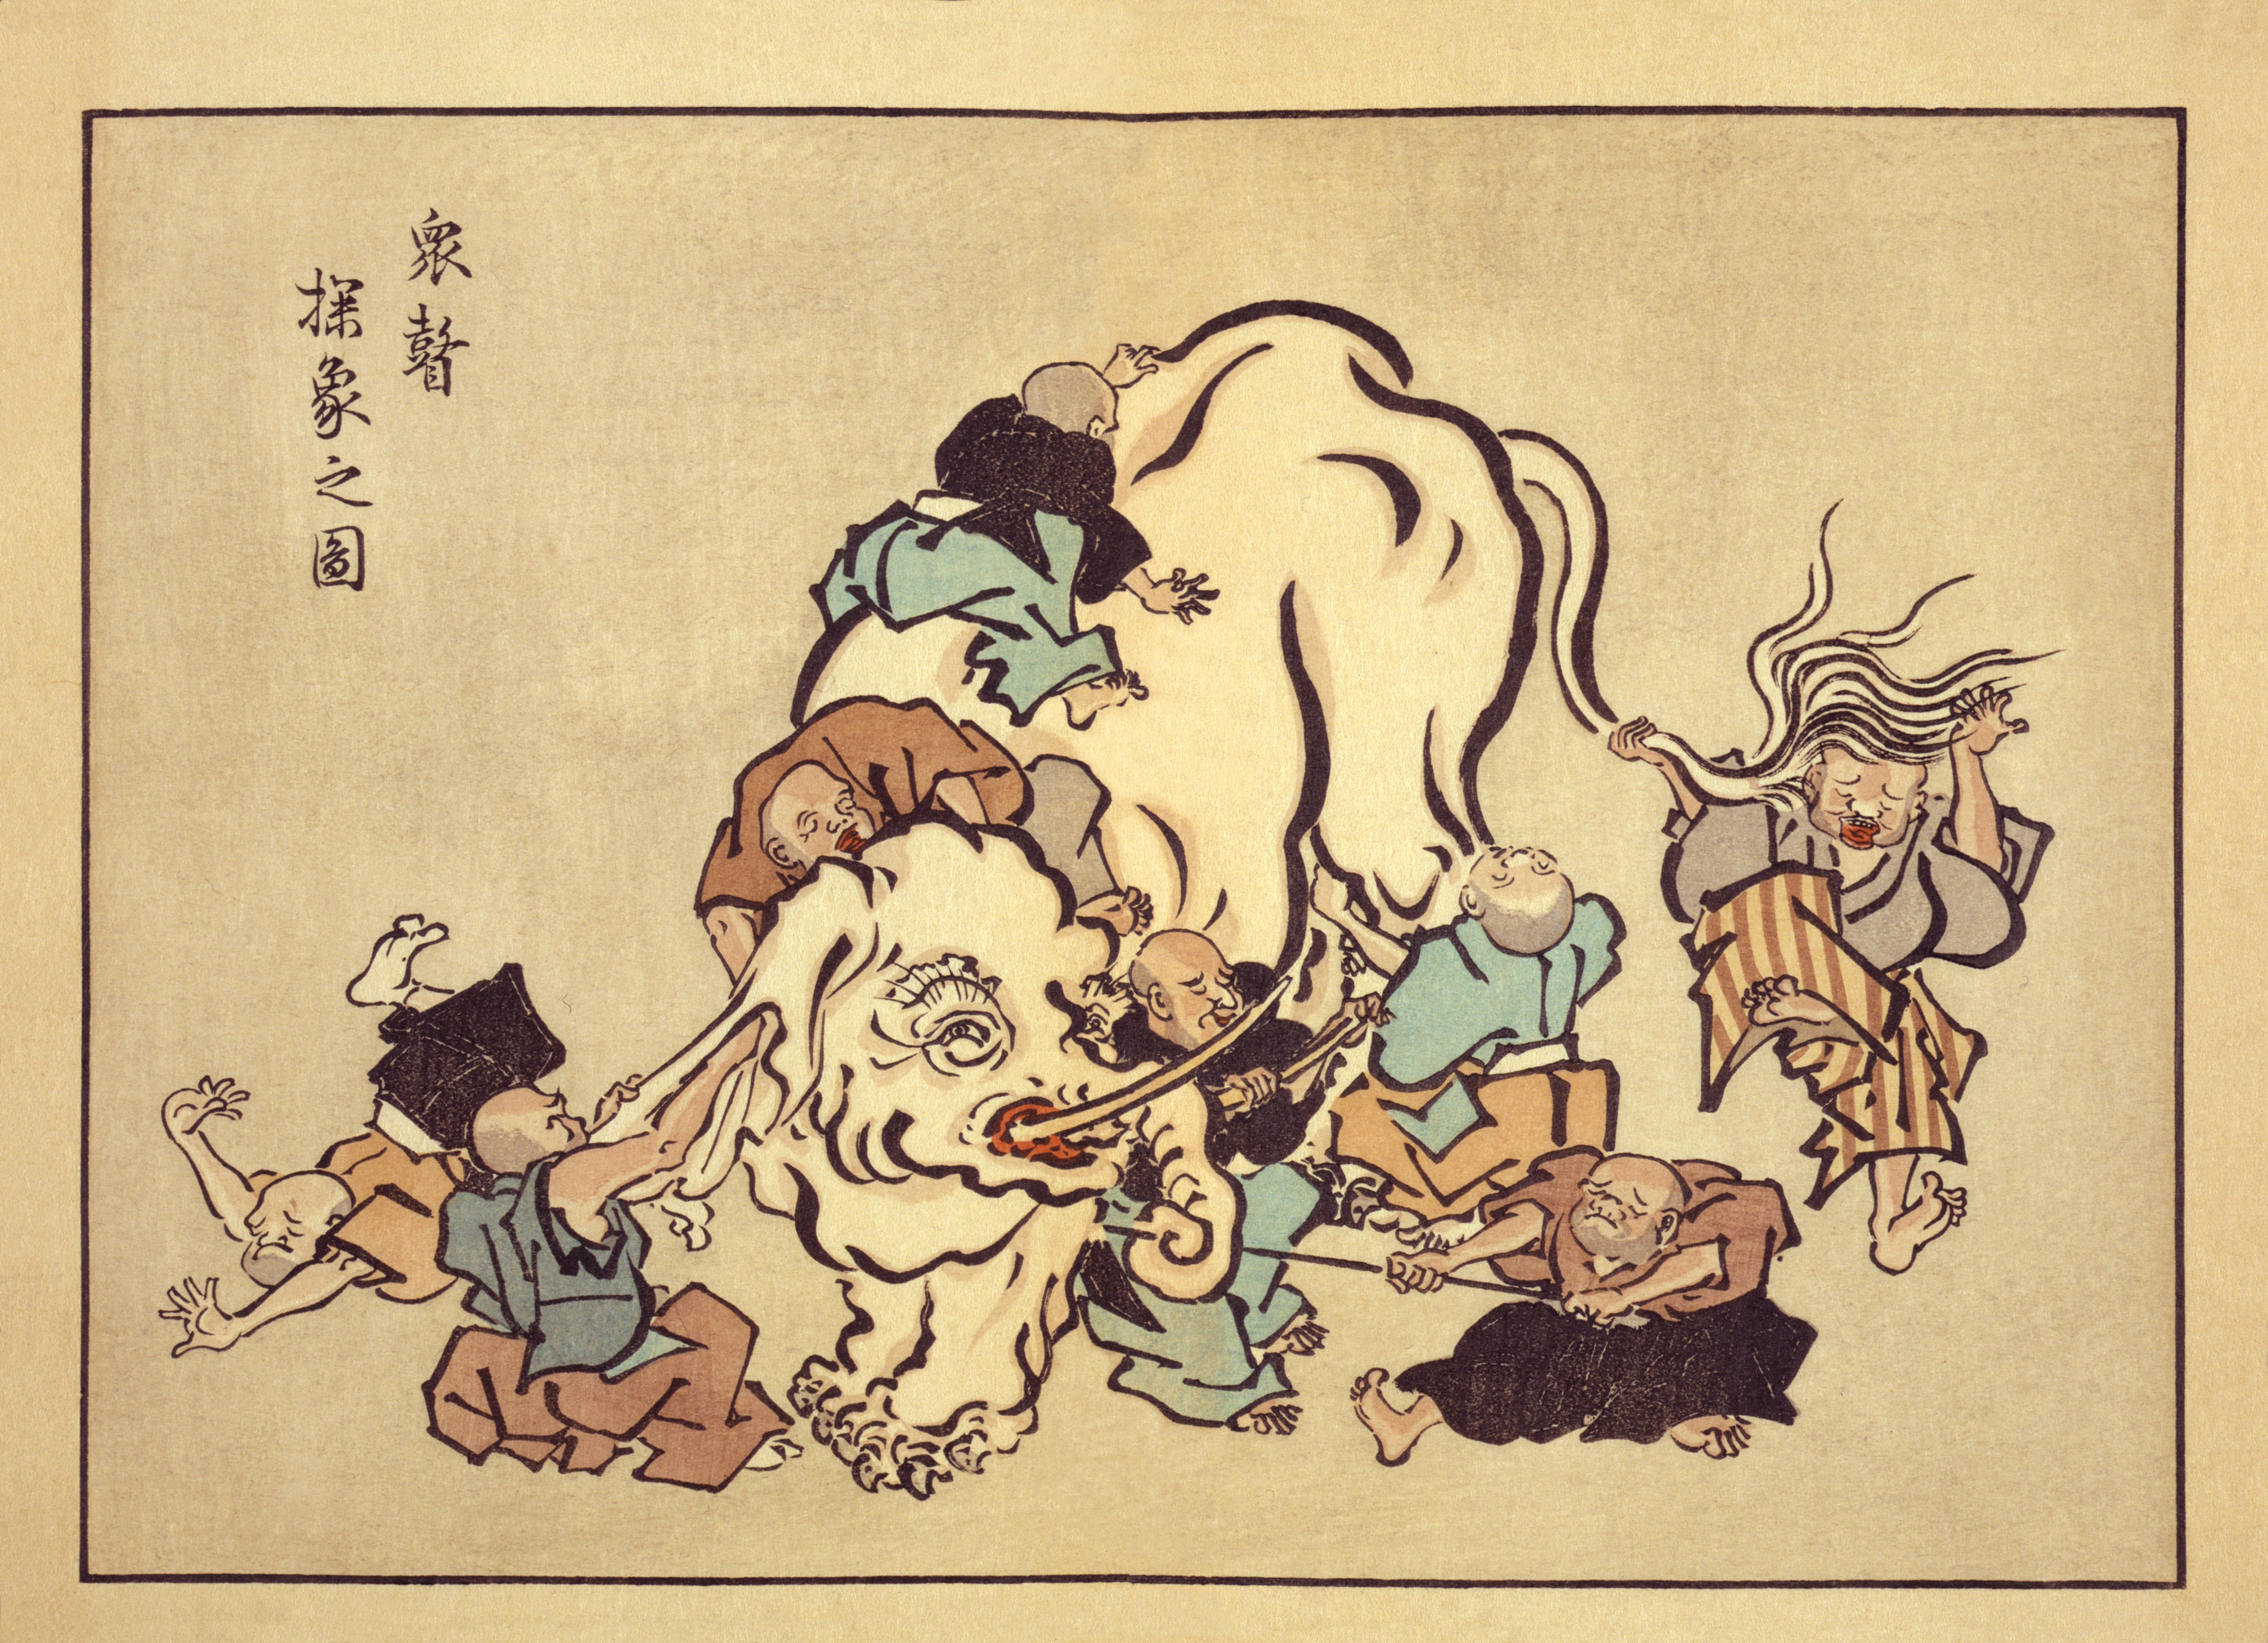
\includegraphics{assets/images/blind-monks.jpg}
  \caption{Blind monks examining the Bitcoin bull}
  \label{fig:blind-monks}
\end{figure}

Bitcoin is a child of many disciplines. Like blind monks examining an elephant,
everyone who approaches this novel technology does so from a different angle.
And everyone will come to different conclusions about the nature of the beast.

The following lessons are about some of my assumptions which Bitcoin shattered,
and the conclusions I arrived at. Philosophical questions of immutability,
scarcity, locality, and identity are explored in the first four lessons.  Every
part consists of seven lessons.

~

\begin{samepage}
Part~\ref{ch:philosophy} -- Philosophy:

\begin{enumerate}
  \item Immutability and change
  \item The scarcity of scarcity
  \item Replication and locality
  \item The problem of identity
  \item An immaculate conception
  \item The power of free speech
  \item The limits of knowledge
\end{enumerate}
\end{samepage}

Lesson \ref{les:5} explores how Bitcoin's origin story is not only fascinating but
absolutely essential for a leaderless system. The last two lessons of this
chapter explore the power of free speech and the limits of our individual
knowledge, reflected by the surprising depth of the Bitcoin rabbit hole.

I hope that you will find the world of Bitcoin as educational, fascinating and
entertaining as I did and still do. I invite you to follow the white rabbit and
explore the depths of this rabbit hole. Now hold on to your pocket watch, pop
down, and enjoy the fall.

\chapter{Immutability and Change}
\label{ch:immutability}

\begin{chapquote}{Lewis Carroll, \textit{Alice in Wonderland}}
I wonder if I´ve been changed in the night. Let me think. Was I the same when I
got up this morning? I almost think I can remember feeling a little different.
But if I'm not the same, the next question is `Who in the world am I?' Ah,
that´s the great puzzle!
\end{chapquote}

Bitcoin is inherently hard to describe. It is a \textit{new thing}, and any
attempt to draw a comparison to previous concepts -- be it by calling
it digital gold or the internet of money -- is bound to fall short of
the whole. Whatever your favorite analogy might be, two aspects of
Bitcoin are absolutely essential: decentralization and immutability.

One way to think about Bitcoin is as an [automated social contract]. The
software is just one piece of the puzzle, and hoping to change Bitcoin
by changing the software is an exercise in futility. One would have to
convince the rest of the network to adopt the changes, which is more a
psychological effort than a software engineering one.

The following might sound absurd at first, like so many other things in
this space, but I believe that it is profoundly true nonetheless: You
won't change Bitcoin, but Bitcoin will change you.

\bigskip

\marginnote{\textit{``Bitcoin will change us more than we will change it.''} -- Marty Bent}
% > <cite>[Marty Bent]</cite>

It took me a long time to realize the profundity of this. Since Bitcoin
is just software and all of it is open-source, you can simply change
things at will, right? Wrong. \textit{Very} wrong. Unsurprisingly, Bitcoin's
creator knew this all too well.

% > The nature of Bitcoin is such that once version 0.1 was released, the
% > core design was set in stone for the rest of its lifetime.
% > <cite>[Satoshi Nakamoto]</cite>

Many people have attempted to change Bitcoin's nature. So far all of
them have failed. While there is an endless sea of forks and altcoins,
the Bitcoin network still does its thing, just as it did when the first
node went online. The altcoins won't matter in the long run. The forks
will eventually starve to death. Bitcoin is what matters. As long as our
fundamental understanding of mathematics and/or physics doesn't change,
the Bitcoin honeybadger will continue to not care.

% > "Bitcoin is the first example of a new form of life. It lives and
% > breathes on the internet. It lives because it can pay people to keep
% > it alive. [...] It can't be changed. It can't be argued with. It
% > can't be tampered with. It can't be corrupted. It can't be stopped.
% > [...] If nuclear war destroyed half of our planet, it would continue
% > to live, uncorrupted. "
% > <cite>[Ralph Merkle]</cite>

The heartbeat of the Bitcoin network will outlast all of ours.

Realizing the above changed me way more than the past blocks of the
Bitcoin blockchain ever will. It changed my time preference, my
understanding of economics, my political views, and so much more. Hell,
it is even [changing people's diets][carnivores]. If all of this sounds crazy to
you, you're in good company. All of this is crazy, and yet it is
happening.

Bitcoin taught me that it won't change. I will.

% ---
%
% #### Through the Looking-Glass
%
% - [Bitcoin's Gravity: How idea-value feedback loops are pulling people in][gravity]
% - [Lesson 18: Move slowly and don't break things][lesson18]
%
% #### Down the Rabbit Hole
%
% - [Unpacking Bitcoin's Social Contract][automated social contract]: A framework for skeptics by Hasu
% - [DAOs, Democracy and Governance][Ralph Merkle] by Ralph C. Merkle
% - [Marty's Bent][bent]: A daily newsletter highlighting signal in Bitcoin by Marty Bent
% - [Technical Discussion on Bitcoin's Transactions and Scripts][Satoshi Nakamoto] by Satoshi Nakamoto, Gavin Andresen, and others
% - [Inside the World of the Bitcoin Carnivores][carnivores]: Why a small community of Bitcoin users is eating meat exclusively by Jordan Pearson
% - [Tales From the Crypt][tftc] hosted by Marty Bent
%
% <!-- Internal -->
% [gravity]: 
% [lesson18]: {{ 'bitcoin/lessons/ch3-18-move-slowly-and-dont-break-things' | absolute_url }}
%
% <!-- Further Reading -->
% [automated social contract]: https://medium.com/@hasufly/bitcoins-social-contract-1f8b05ee24a9
% [carnivores]: https://motherboard.vice.com/en_us/article/ne74nw/inside-the-world-of-the-bitcoin-carnivores
% [tftc]: https://tftc.io/tales-from-the-crypt/
% [bent]: https://tftc.io/martys-bent/
%
% <!-- Quotes -->
% [Ralph Merkle]: http://merkle.com/papers/DAOdemocracyDraft.pdf
% [Satoshi Nakamoto]: https://bitcointalk.org/index.php?topic=195.msg1611#msg1611
%
% <!-- Twitter People -->
% [Marty Bent]: https://twitter.com/martybent
%
% <!-- Wikipedia -->
% [alice]: https://en.wikipedia.org/wiki/Alice%27s_Adventures_in_Wonderland
% [carroll]: https://en.wikipedia.org/wiki/Lewis_Carroll

---
layout: lesson
title: Lesson 2
subtitle: The scarcity of scarcity
quote: "That's quite enough — I hope I sha'n't grow any more..."
categories: [bitcoin, lesson]
audio: /assets/audio/21lessons/1-02.m4a 
---

In general, the advance of technology seems to make things more
abundant. More and more people are able to enjoy what previously have
been luxurious goods. Soon, we will all live like kings. Most of us
already do. As Peter Diamandis wrote in [Abundance]: "Technology is a
resource-liberating mechanism. It can make the once scarce the now
abundant."

Bitcoin, an advanced technology in itself, breaks this trend and creates
a new commodity which is truly scarce. Some even argue that it is one of
the scarcest things in the universe. The supply can't be inflated, no
matter how much effort one chooses to expend towards creating more.

> "Only two things are genuinely scarce: time and bitcoin."
> <cite>[Saifedean Ammous][bitcoin-standard-presentation]</cite>

Paradoxically, it does so by a mechanism of copying. Transactions are
broadcast, blocks are propagated, the distributed ledger is --- well,
you guessed it --- distributed. All of these are just fancy words for
copying. Heck, Bitcoin even copies itself onto as many computers as it
can, by incentivizing individual people to run full nodes and mine new
blocks.

All of this duplication wonderfully works together in a concerted effort
to produce scarcity.

In a time of abundance, Bitcoin taught me what real scarcity is.

---

#### Through the Looking-Glass

- [Lesson 14: Sound money][lesson14]

#### Down the Rabbit Hole

- [The Bitcoin Standard: The Decentralized Alternative to Central Banking][bitcoin-standard]
- [Abundance: The Future Is Better Than You Think][Abundance] by Peter Diamandis
- [Presentation on The Bitcoin Standard][bitcoin-standard-presentation] by Saifedean Ammous
- [Modeling Bitcoin's Value with Scarcity][planb-scarcity] by PlanB
- 🎧 [Misir Mahmudov on the Scarcity of Time & Bitcoin][tftc60] TFTC #60 hosted by Marty Bent
- 🎧 [PlanB – Modelling Bitcoin's digital scarcity through stock-to-flow techniques][slp67] SLP #67 hosted by Stephan Livera

<!-- Through the Looking-Glass -->
[lesson14]: {{ 'bitcoin/lessons/ch2-14-sound-money' | absolute_url }}

<!-- Down the Rabbit Hole -->
[Abundance]: https://www.diamandis.com/abundance
[bitcoin-standard]: http://amzn.to/2L95bJW
[bitcoin-standard-presentation]: https://www.bayernlb.de/internet/media/de/ir/downloads_1/bayernlb_research/sonderpublikationen_1/bitcoin_munich_may_28.pdf
[planb-scarcity]: https://medium.com/@100trillionUSD/modeling-bitcoins-value-with-scarcity-91fa0fc03e25
[tftc60]: https://anchor.fm/tales-from-the-crypt/episodes/Tales-from-the-Crypt-60-Misir-Mahmudov-e3aibh
[slp67]: https://stephanlivera.com/episode/67

<!-- Wikipedia -->
[alice]: https://en.wikipedia.org/wiki/Alice%27s_Adventures_in_Wonderland
[carroll]: https://en.wikipedia.org/wiki/Lewis_Carroll

\chapter{Replikation und Lokalität}
\label{les:3}

\begin{chapquote}{Lewis Carroll, \textit{Alice im Wunderland}}
Demnächst kam eine ärgerliche Stimme -- die des Kaninchens -- \enquote{Pat! Pat! wo bist du?}
\end{chapquote}

Die Quantenmechanik außen vor gelassen, ist die Lokalisierung kein echtes
Problem in unserer physischen Welt. Die Frage \textit{\enquote{Wo ist X?}} kann
sinnvoll beantwortet werden, egal ob X eine Person oder ein Objekt ist. In der
digitalen Welt ist die Frage, \textit{wo} man sich befindet bereits schwierig,
aber nicht unmöglich zu beantworten. Wo sind deine E-Mails wirklich? Eine
schlechte Antwort wäre \enquote{in der Cloud}, da diese nur der Computer eines
anderen ist. Dennoch, wenn du alle Speichermedien welche deine Mails aufzeichnet
finden willst, könntest du diese theoretisch finden.

Bei Bitcoin ist die Frage nach dem \enquote{Wo} wirklich knifflig. Wo genau sind
deine Bitcoins?

\begin{quotation}\begin{samepage}
\enquote{
Ich öffnete die Augen sah mich um und stellte die unvermeidliche, die
traditionelle, die bedauerlicherweise abgedroschene postoperative Frage:
\enquote{Wo bin ich?}
}
\begin{flushright} -- Daniel Dennett\footnote{Daniel Dennett, \textit{Where Am I?}~\cite{where-am-i}}
\end{flushright}\end{samepage}\end{quotation}

Die Frage stellt sich aus zweifacher Hinsicht: Erstens wird der
\enquote{distributed Ledger} (die \enquote{verteilte Kontenübersicht}) durch
vollständige Replikation verteilt, d.h. diese Kontenübersicht ist überall.
Zweitens gibt es keine Bitcoins. Nicht nur physisch, sondern auch technisch
gesehen nicht.

Bitcoin behält den Überblick über einen Satz von \enquote{\textit{unspent
transaction outputs}} (UTXOs) ohne sich jemals auf eine Entität beziehen zu
müssen, die einen Bitcoin repräsentiert. Die Existenz eines Bitcoin wird von
diesen UTXOs abgeleitet: jeder Eintrag mit 100 Millionen Basiseinheiten wird als
Bitcoin bezeichnet.

\begin{quotation}\begin{samepage}
\enquote{Wo ist es in diesem Moment, im Transit? [\ldots] Erstens, es gibt keine
Bitcoins. Es gibt sie einfach nicht. Sie existieren nicht. Es gibt
Ledger-Einträge in einem Ledger, der gemeinsam genutzt wird [\ldots] Sie
existieren nicht an einem physischen Ort. Der Ledger existiert im Wesentlichen
an jedem physischen Ort. Geographie macht hier keinen Sinn --- sie wird dir
nicht helfen dein Regelwerk festzulegen.}
\begin{flushright} -- Peter Van Valkenburgh\footnote{Peter Van Valkenburgh zu Gast bei dem \textit{What Bitcoin Did} Podcast, Episode 49 \cite{wbd049}}
\end{flushright}\end{samepage}\end{quotation}

Also was besitzt du eigentlich wenn du sagst: \textit{\enquote{Ich habe einen
Bitcoin}}, wenn es keine Bitcoins gibt? Nun erinnerst du dich an all diese
komischen Worte, die du bei der Einrichtung deiner Wallet aufschreiben musstest?
Wie sich herausstellt, sind dies die Zauberworte und das was du besitzt ist ein
Zauber mit dem du Einträge in das Bitcoin-Kontenbuch machen kannst — die
Schlüssel um Bitcoins zu \enquote{bewegen}. Deshalb sind deine privaten
Schlüssel im Grunde genommen deine Bitcoins. Wenn du denkst, dass ich mir das
alles ausgedacht habe, kannst du mir gerne deine privaten Schlüssel schicken.

\paragraph{Bitcoin hat mir beigebracht, dass Lokalität eine knifflige
Angelegenheit ist.}

% ---
%
% #### Through the Looking-Glass
%
% - [The Magic Dust of Cryptography: How digital information is changing our society][a magic spell]
%
% #### Down the Rabbit Hole
%
% - [Where Am I?][Daniel Dennett] by Daniel Dennett
% - 🎧 [Peter Van Valkenburg on Preserving the Freedom to Innovate with Public Blockchains][wbd049] WBD #49 hosted by Peter McCormack
%
% <!-- Through the Looking-Glass -->
% [a magic spell]: 
%
% <!-- Down the Rabbit Hole -->
% [Daniel Dennett]: https://www.lehigh.edu/~mhb0/Dennett-WhereAmI.pdf
% [1st Amendment]: https://en.wikipedia.org/wiki/First_Amendment_to_the_United_States_Constitution
% [wbd049]: https://www.whatbitcoindid.com/podcast/coin-centers-peter-van-valkenburg-on-preserving-the-freedom-to-innovate-with-public-blockchains
%
% <!-- Wikipedia -->
% [alice]: https://en.wikipedia.org/wiki/Alice%27s_Adventures_in_Wonderland
% [carroll]: https://en.wikipedia.org/wiki/Lewis_Carroll

\chapter{The Problem of Identity}
\label{les:4}

\begin{chapquote}{Lewis Carroll, \textit{Alice in Wonderland}}
  ``Who are you?'' said the caterpillar.
\end{chapquote}

Nic Carter, in an homage to Thomas Nagel's treatment of the same
question in regards to a bat, wrote an excellent piece which discusses
the following question: What is it like to be a bitcoin? He
brilliantly shows that open, public blockchains in general, and Bitcoin
in particular, suffer from the same conundrum as the Ship of
Theseus: which Bitcoin is the real Bitcoin?

\begin{quotation}
``Consider just how little persistence Bitcoin's components have. The
entire codebase has been reworked, altered, and expanded such that it
barely resembles its original version. [...] The registry of who
owns what, the ledger itself, is virtually the only persistent trait
of the network [...]
To be considered truly leaderless, you must surrender the easy
solution of having an entity that can designate one chain as the
legitimate one.''
\flushright -- Nic Carter\footnote{Nic Carter, \textit{What is it like to be a bitcoin?} \cite{bitcoin-identity}}
\end{quotation}

It seems like the advancement of technology keeps forcing us to take
these philosophical questions seriously. Sooner or later, self-driving
cars will be faced with real-world versions of the trolley problem,
forcing them to make ethical decisions about whose lives do matter and
whose do not.

Cryptocurrencies, especially since the first contentious hard-fork,
force us to think about and agree upon the metaphysics of identity.
Interestingly, the two biggest examples we have so far have lead to two
different answers. On August 1, 2017, Bitcoin split into two camps. The
market decided that the unaltered chain is the original Bitcoin. One
year earlier, on October 25, 2016, Ethereum split into two camps. The
market decided that the \textit{altered} chain is the original Ethereum.

If properly decentralized, the questions posed by the \textit{Ship of Theseus}
will have to be answered in perpetuity for as long as these networks of
value-transfer exist.

\paragraph{Bitcoin taught me that decentralization contradicts identity.}

% ---
%
% #### Down the Rabbit Hole
%
% - [What Is It Like to be a Bat?][in regards to a bat] by Thomas Nagel
% - [What is it like to be a bitcoin?] by Nic Carter
% - [Ship of Theseus], [trolley problem] on Wikipedia
%
% [in regards to a bat]: https://en.wikipedia.org/wiki/What_Is_it_Like_to_Be_a_Bat%3F
% [What is it like to be a bitcoin?]: https://medium.com/s/story/what-is-it-like-to-be-a-bitcoin-56109f3e6753
% [Ship of Theseus]: https://en.wikipedia.org/wiki/Ship_of_Theseus
% [trolley problem]: https://en.wikipedia.org/wiki/Trolley_problem
%
% <!-- Wikipedia -->
% [alice]: https://en.wikipedia.org/wiki/Alice%27s_Adventures_in_Wonderland
% [carroll]: https://en.wikipedia.org/wiki/Lewis_Carroll

---
layout: lesson
title: Lesson 5
subtitle: An immaculate conception
quote: "\"Their heads are gone,\" the soldiers shouted in reply..."
categories: [bitcoin, lesson]
audio: /assets/audio/21lessons/1-05.m4a 
---

Everyone loves a good origin story. The origin story of Bitcoin is a
fascinating one, and the details of it are more important than one might
think at first. Who is Satoshi Nakamoto? Was he one person or a group of
people? Was he a she? Time-traveling alien, or advanced AI? Outlandish
theories aside, we will probably never know. And this is important.

Satoshi chose to be anonymous. He planted the seed of Bitcoin. He stuck
around for long enough to make sure the network won't die in its
infancy. And then he vanished.

What might look like a weird anonymity stunt is actually crucial for a
truly decentralized system. No centralized control. No centralized
authority. No inventor. No-one to prosecute, torture, blackmail, or
extort. An immaculate conception of technology.

> "One of the greatest things that Satoshi did was disappear."
> <cite>[Jimmy Song]</cite>

Since the birth of Bitcoin, thousands of other cryptocurrencies were
created. None of these clones share its origin story. If you want to
supersede Bitcoin, you will have to transcend its origin story. In a war
of ideas, narratives dictate survival.

> "Gold was first fashioned into jewelry and used for barter over 7,000
> years ago. Gold's captivating gleam led to it being considered a gift
> from the gods."
> <cite>[Gold: The Extraordinary Metal]</cite>

Like gold in ancient times, Bitcoin might be considered a gift from the
gods. Unlike gold, Bitcoins origins are all too human. And this time, we
know who the gods of development and maintenance are: people all over
the world, anonymous or not.

Bitcoin taught me that narratives are important.

---

#### Down the Rabbit Hole

- [Why Bitcoin is different][Jimmy Song] by Jimmy Song
- [Gold: The Extraordinary Metal] by the Austrian Mint

<!-- Down the Rabbit Hole -->
[Jimmy Song]: https://medium.com/@jimmysong/why-bitcoin-is-different-e17b813fd947
[Gold: The Extraordinary Metal]: https://www.muenzeoesterreich.at/eng/discover/for-investors/gold-the-extraordinary-metal

<!-- Wikipedia -->
[alice]: https://en.wikipedia.org/wiki/Alice%27s_Adventures_in_Wonderland
[carroll]: https://en.wikipedia.org/wiki/Lewis_Carroll

---
layout: lesson
title: Lesson 6
subtitle: The power of free speech
quote: "\"I beg your pardon?\" said the mouse, frowning, but very politely, \"did you speak?\""
categories: [bitcoin, lesson]
audio: /assets/audio/21lessons/1-06.m4a 
---

Bitcoin is an idea. An idea which, in its current form, is the
manifestation of a machinery purely powered by text. Every aspect of
Bitcoin is text: The whitepaper is text. The software which is run by
its nodes is text. The ledger is text. Transactions are text. Public and
private keys are text. Every aspect of Bitcoin is text, and thus
equivalent to speech.

> "Congress shall make no law respecting an establishment of religion,
> or prohibiting the free exercise thereof; or abridging the freedom of
> speech, or of the press; or the right of the people peaceably to
> assemble, and to petition the Government for a redress of grievances."
> <cite>[First Amendment to the United States Constitution][1st Amendment]</cite>

Although the final battle of the [Crypto Wars] has not been fought yet,
it will be very difficult to criminalize an idea, let alone an idea
which is based on the exchange of text messages. Every time a government
tries to outlaw text or speech, we slip down a path of absurdity which
inevitably leads to abominations like [illegal numbers] and [illegal
primes].

As long as there is a part of the world where speech is free as in
*freedom*, Bitcoin is unstoppable.

> "There is no point in any Bitcoin transaction that Bitcoin ceases to
> be *text.* It is *all* *text*, all the time. [...]
>
> Bitcoin is **text.** Bitcoin is **speech.** It cannot be regulated in
> a free country like the USA with guaranteed inalienable rights and a
> First Amendment that explicitly excludes the act of publishing from
> government oversight."
> <cite>[Beautyon]</cite>

Bitcoin taught me that in a free society, free speech and free software
are unstoppable.

---

#### Through the Looking-Glass

- [The Magic Dust of Cryptography: How digital information is changing our society][a magic spell]

#### Down the Rabbit Hole

- [Why America can't regulate Bitcoin][Beautyon] by Beautyon
- [First Amendment to the United States Constitution][1st Amendment], [Crypto Wars], [illegal numbers], [illegal primes] on Wikipedia

<!-- Through the Looking-Glass -->
[a magic spell]:   

<!-- Down the Rabbit Hole -->
[1st Amendment]: https://en.wikipedia.org/wiki/First_Amendment_to_the_United_States_Constitution
[Crypto Wars]: https://en.wikipedia.org/wiki/Crypto_Wars
[illegal numbers]: https://en.wikipedia.org/wiki/Illegal_number
[illegal primes]: https://en.wikipedia.org/wiki/Illegal_prime
[Beautyon]: https://hackernoon.com/why-america-cant-regulate-bitcoin-8c77cee8d794

<!-- Wikipedia -->
[alice]: https://en.wikipedia.org/wiki/Alice%27s_Adventures_in_Wonderland
[carroll]: https://en.wikipedia.org/wiki/Lewis_Carroll

\chapter{ The Limits of Knowledge}
\label{les:7}

\begin{chapquote}{Lewis Carroll, \textit{Alice in Wonderland}}
``Down, down, down. Would the fall never come to an end?''
\end{chapquote}

Getting into Bitcoin is a humbling experience. I thought that I knew
things. I thought that I was educated. I thought that I knew my computer
science, at the very least. I studied it for years, so I have to know
everything about digital signatures, hashes, encryption, operational
security, and networks, right?

Wrong.

Learning all the fundamentals which make Bitcoin work is hard.
Understanding all of them deeply is borderline impossible.

\begin{quotation}
``No one has found the bottom of the Bitcoin rabbit hole.''
\end{quotation}
% > <cite>[Jameson Lopp]</cite>

My list of books to read keeps expanding way quicker than I could
possibly read them. The list of papers and articles to read is virtually
endless. There are more podcasts on all of these topics than I could
ever listen to. It truly is humbling. Further, Bitcoin is evolving and
it's almost impossible to stay up-to-date with the accelerating rate of
innovation. The dust of the first layer hasn't even settled yet, and
people have already built the second layer and are working on the third.

\paragraph{Bitcoin taught me that I know very little about almost anything. It
taught me that this rabbit hole is bottomless.}

% ---
%
% #### Down the Rabbit Hole
%
% - [Bitcoin Literature] by the Satoshi Nakamoto Institute
% - [Bitcoin Information & Resources][lopp-resources] by Jameson Lopp
% - [Educational Resources][bitcoin-only] by Bitcoin Only
%
% <!-- Twitter -->
% [Jameson Lopp]: https://twitter.com/lopp/status/1061415918616698881
%
% <!-- Down the Rabbit Hole -->
% [lopp-resources]: https://www.lopp.net/bitcoin-information.html
% [bitcoin-only]: https://bitcoin-only.com/#learning
% [Bitcoin Literature]: https://nakamotoinstitute.org/literature/
%
% <!-- Wikipedia -->
% [alice]: https://en.wikipedia.org/wiki/Alice%27s_Adventures_in_Wonderland
% [carroll]: https://en.wikipedia.org/wiki/Lewis_Carroll

% 
\part{Economics}
\label{ch:economics}

\begin{chapquote}{Lewis Carroll, \textit{Alice in Wonderland}}
``A large rose tree stood near the entrance of the garden: the roses on it were
white, but there were three gardeners at it, busily painting them red. This
Alice thought a very curious thing...''
\end{chapquote}

\textit{Money doesn’t grow on trees.} To believe that it does is foolish, and our
parents make sure that we know about that by repeating this saying like a
mantra. We are encouraged to use money wisely, to not spend it frivolously,
and to save it in good times to help us through the bad. Money, after all,
does not grow on trees.

Bitcoin taught me more about money than I ever thought I would need to know.
Through it, I was forced to explore the history of money, banking, various
schools of economic thought, and many other things. The quest to understand
Bitcoin lead me down a plethora of paths, some of which I try to explore in
this series.

In the first seven lessons some of the philosophical questions Bitcoin touches
on were discussed. The next seven lessons will take a closer look at money and
economics.

~

Part II -- Economics:

\begin{enumerate}
  \item Financial ignorance
  \item Inflation
  \item Value
  \item Money
  \item The history and downfall of money
  \item Fractional reserve insanity
  \item Sound money
\end{enumerate}

Again, I will only be able to scratch the surface. Bitcoin is not only
ambitious, but also broad and deep in scope, making it impossible to cover all
relevant topics in a single lesson, essay, article, or book. I  doubt if it is
even possible at all.

\textit{Bitcoin is a new form of money}, which makes learning about
economics paramount to understanding it. Dealing with the nature of human action
and the interactions of economic agents, economics is probably one of the
largest and fuzziest pieces of the Bitcoin puzzle.

Again, these lessons are an exploration of the various things I have learned
from Bitcoin. They are a personal reflection of my journey down the rabbit hole.
Having no background in economics, I am definitely out of my comfort zone and
especially aware that any understanding I might have is incomplete. I will do my
best to outline what I have learned, even at the risk of making a fool out of
myself. After all, I am still trying to answer the question: ``What have you
learned from Bitcoin?''

\begin{figure}
  \centering
  
\includegraphics[width=8cm]{assets/images/the-tweet.png}
  \caption{What have you learned from Bitcoin?}
  \label{fig:the-tweet}
\end{figure}

After seven lessons examined through the lens of philosophy, let’s use the lens
of economics to look at seven more. Economy class is all I can offer this time.
Final destination: \textit{sound money}.

% [the question]: https://twitter.com/arjunblj/status/1050073234719293440

% \chapter{Financial Ignorance}
\label{les:8}

\begin{chapquote}{Lewis Carroll, \textit{Alice im Wunderland}}
\enquote{And what an ignorant little girl she'll think me for asking! No, it'll never
do to ask: perhaps I shall see it written up somewhere.}
\end{chapquote}

One of the most surprising things, to me, was the amount of finance,
economics, and psychology required to get a grasp of what at first
glance seems to be a purely \textit{technical} system --- a computer network.
To paraphrase a little guy with hairy feet: \enquote{It's a dangerous business,
Frodo, stepping into Bitcoin. You read the whitepaper, and if you don't
keep your feet, there's no knowing where you might be swept off to.}

To understand a new monetary system, you have to get acquainted with the
old one. I began to realize very soon that the amount of financial
education I enjoyed in the educational system was essentially \textit{zero}.

\paragraph{}
Like a five-year-old, I began to ask myself a lot of questions: How does the
banking system work? How does the stock market work? What is fiat money? What is
\textit{regular} money? Why is there so much
debt?\footnote{\url{https://www.usdebtclock.org/}} How much money is actually
printed, and who decides that?

\newpage

After a mild panic about the sheer scope of my ignorance, I found
reassurance in realizing that I was in good company.

\begin{quotation}\begin{samepage}
\enquote{Isn't it ironic that Bitcoin has taught me more about money than all these
years I've spent working for financial institutions? \ldots including starting my
career at a central bank}
\begin{flushright} -- Aaron\footnote{Aaron (\texttt{@aarontaycc}, \texttt{@fiatminimalist}), tweet from Dec.
12, 2018~\cite{aarontaycc-tweet}}
\end{flushright}\end{samepage}\end{quotation}

\begin{quotation}\begin{samepage}
\enquote{I've learned more about finance, economics, technology, cryptography, human
psychology, politics, game theory, legislation, and myself in the last three
months of crypto than the last three and a half years of college}
\begin{flushright} -- Dunny\footnote{Dunny (\texttt{@BitcoinDunny}), tweet from Nov. 28,
2017~\cite{bitcoindunny-tweet}}
\end{flushright}\end{samepage}\end{quotation}

These are just two of the many confessions all over twitter.\footnote{See
\url{http://bit.ly/btc-learned} for more confessions on twitter.} Bitcoin, as
was explored in Lesson \ref{les:1}, is a living thing. Mises argued that
economics also is a living thing. And as we all know from personal experience,
living things are inherently difficult to understand.

\begin{quotation}\begin{samepage}
\enquote{A scientific system is but one station in an endlessly progressing
search for knowledge. It is necessarily affected by the insufficiency
inherent in every human effort. But to acknowledge these facts does
not mean that present-day economics is backward. It merely means that
economics is a living thing --- and to live implies both imperfection
and change.}
\begin{flushright} -- Ludwig von Mises\footnote{Ludwig von Mises, \textit{Human Action}
\cite{human-action}}
\end{flushright}\end{samepage}\end{quotation}

\newpage

We all read about various financial crises in the news, wonder about how
these big bailouts work and are puzzled over the fact that no one ever
seems to be held accountable for damages which are in the trillions. I
am still puzzled, but at least I am starting to get a glimpse of what is
going on in the world of finance.

Some people even go as far as to attribute the general ignorance on
these topics to systemic, willful ignorance. While history, physics,
biology, math, and languages are all part of our education, the world of
money and finance surprisingly is only explored superficially, if at
all. I wonder if people would still be willing to accrue as much debt as
they currently do if everyone would be educated in personal finance and
the workings of money and debt. Then I wonder how many layers of
aluminum make an effective tinfoil hat. Probably three.

\begin{quotation}\begin{samepage}
\enquote{Those crashes, these bailouts, are not accidents. And neither is it an
accident that there is no financial education in school. [...] It's
premeditated. Just as prior to the Civil War it was illegal to educate a slave,
we are not allowed to learn about money in school.}
\begin{flushright} -- Robert Kiyosaki\footnote{Robert Kiyosaki, \textit{Why the Rich
are Getting Richer}\cite{robert-kiyosaki}}
\end{flushright}\end{samepage}\end{quotation}

Like in The Wizard of Oz, we are told to pay no attention to the man behind the
curtain. Unlike in The Wizard of Oz, we now have real
wizardry\footnote{\url{http://bit.ly/btc-wizardry}}: a censorship-resistant,
open, borderless network of value-transfer. There is no curtain, and the magic
is visible to anyone.\footnote{\url{https://github.com/bitcoin/bitcoin}}

\paragraph{Bitcoin taught me to look behind the curtain and face my financial
ignorance.}

% ---
%
% #### Down the Rabbit Hole
%
% - [Human Action][Ludwig von Mises] by Ludwig von Mises
% - [Why the Rich are Getting Richer][Robert Kiyosaki] by Robert Kiyosaki
%
% [real wizardry]: https://external-preview.redd.it/8d03MWWOf2HIyKrT8ThBGO4WFv-u25JaYqhbEO9b1Sk.jpg?width=683&auto=webp&s=dc5922d84717c6a94527bafc0189fd4ca02a24bb
% [visible to anyone]: https://github.com/bitcoin/bitcoin
%
% <!-- Wikipedia -->
% [alice]: https://en.wikipedia.org/wiki/Alice%27s_Adventures_in_Wonderland
% [carroll]: https://en.wikipedia.org/wiki/Lewis_Carroll

% \chapter{Inflation}
\label{les:9}

\begin{chapquote}{Die Königin der Herzen}
\enquote{Nun, hier muß man nämlich so schnell rennen, wie man kann, um auf der
Stelle zu bleiben. Wenn man irgendwo anders hin will, muß man mindestens doppelt
so schnell rennen.}
\end{chapquote}

Der Versuch die monetäre Inflation zu verstehen und zu verstehen, wie ein
nicht-inflationäres System wie Bitcoin die Art und Weise wie wir Dinge handhaben
verändern könnte, war der Startschuss für meine Reise in die Wirtschaft. Ich
wusste, dass die Inflation die Rate war mit der neues Geld geschaffen wurde aber
ich wusste nicht viel mehr darüber.

Während einige Ökonomen argumentieren, dass Inflation eine gute Sache ist,
argumentieren andere, dass \enquote{hartes} Geld, das nicht einfach vermehrt
werden kann — wie wir es in den Tagen des Goldstandards hatten --- für eine
gesunde Wirtschaft unerlässlich ist. Bitcoin, mit einem endlichen Vorrat von
insgesamt 21 Millionen BTC stimmt mit dem letztgenannten Lager überein.

Normalerweise sind die Auswirkungen der Inflation nicht sofort erkennbar.
Abhängig von der Inflationsrate (und anderen Faktoren) kann die Zeitdauer
zwischen Ursache und Wirkung mehrere Jahre betragen. Aber nicht nur das, die
Inflation hat sogar auf manche Gruppen von Menschen stärkeren Einfluss als auf
andere. Henry Hazlitt betont in \textit{Economics in One Lesson}: \enquote{Die
Kunst der Ökonomie besteht darin, nicht nur die unmittelbaren, sondern die
längeren Auswirkungen eines jeden Handelns oder einer Maßnahme zu betrachten;
sie besteht darin, die Folgen dieser Politik nicht nur für eine Gruppe, sondern
für alle Gruppen nachzuvollziehen.}

Einer meiner persönlichen AHA-Momente war die Erkenntnis, dass die Ausgabe neuer
Währung --- also das Drucken von mehr Geld --- eine \textit{ganz} andere
wirtschaftliche Aktivität ist, als alle anderen wirtschaftlichen Aktivitäten.
Während reale Güter und reale Dienstleistungen einen realen Wert für reale
Menschen erzeugen, tut das Drucken von Geld effektiv genau das Gegenteil: Es
mindert den Wertbestand von jedem, der die inflationierende Währung besitzt.

\begin{quotation}\begin{samepage}
\enquote{Bloße Inflation --- also die bloße Ausgabe von mehr Geld mit der Folge
höherer Löhne und Preise --- kann wie die Schaffung von mehr Nachfrage aussehen.
Aber in Bezug auf die tatsächliche Produktion und den Austausch von realen
Dingen ist es das nicht.}
\begin{flushright} -- Henry Hazlitt\footnote{Henry Hazlitt, \textit{Economics in
One Lesson} \cite{hazlitt}}
\end{flushright}\end{samepage}\end{quotation}

Die zerstörerische Kraft der Inflation wird deutlich, sobald aus ein wenig
Inflation eine \textit{ganze Menge} Inflation wird. Wenn Geld
hyperinflationiert~\cite{wiki:hyperinflation} werden die Dinge sehr schnell sehr
grässlich.\footnote{\url{https://en.wikipedia.org/wiki/Hyperinflation}} Da die
aufgeblähte Währung zusammenbricht kann sie im Laufe der Zeit keinen Wert mehr
speichern und die Menschen werden versuchen anstatt der Währung alle
möglichen Waren in die Hände zu bekommen.

\paragraph{}
Eine weitere Folge der Hyperinflation ist, dass all das Geld welches die
Menschen im Laufe ihres Lebens gespart haben verschwindet. Das Papiergeld in den
Brieftaschen wird natürlich immer noch da sein. Aber es wird genau das sein:
wertloses Papier.

\begin{figure}
  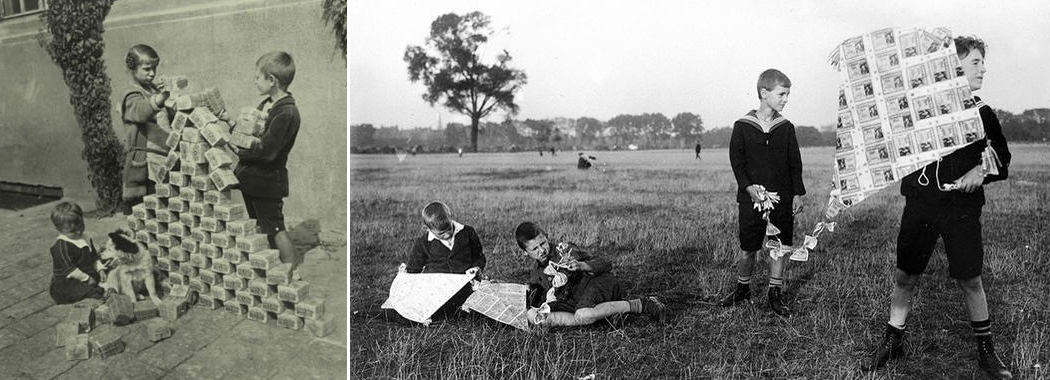
\includegraphics{assets/images/children-playing-with-money.png}
  \caption{Hyperinflation in der Weimarer Republik (1921-1923)}
  \label{fig:children-playing-with-money}
\end{figure}

\paragraph{}
Das Geld verliert auch bei einer \textit{milden} Inflation seinen Wert. Es
geschieht nur langsam genug, so dass die meisten Menschen die Abnahme der
Kaufkraft nicht bemerken. Sobald die Druckmaschinen einmal laufen ist es
schwierig die Inflation einer Währung aufzuhalten, und was soeben noch eine
milde Inflation war, kann sich per Knopfdruck in eine starke Inflation
verwandeln. Wie Friedrich Hayek in einem seiner Essays betonte, führt eine milde
Inflation in der Regel zu einer völligen Inflation.

\begin{quotation}\begin{samepage}
\enquote{Eine \enquote{milde} kontinuierliche Inflation kann nicht helfen — sie
kann nur zu einer völligen Inflation führen.}
\begin{flushright} -- Friedrich Hayek\footnote{Friedrich Hayek, \textit{1980s
Unemployment and the Unions} \cite{hayek-inflation}}
\end{flushright}\end{samepage}\end{quotation}

Die Inflation ist besonders tückisch, da sie diejenigen begünstigt die näher an
den Druckmaschinen sitzen. Es braucht Zeit bis das neu geschaffene Geld
zirkuliert und die Preise angepasst werden. Wenn du es also schaffst mehr Geld
in die Hände zu bekommen, noch bevor das aller anderen an Wert verliert, bist du
der Inflationskurve ein Stück voraus. Aus diesem Grund kann die Inflation auch
als versteckte Steuer angesehen werden, denn am Ende profitieren die Regierungen
davon während alle anderen den Preis dafür bezahlen.

\begin{quotation}\begin{samepage}
\enquote{Ich denke nicht, dass es eine Übertreibung ist zu sagen, dass die
Geschichte weitgehend eine Geschichte der Inflation ist und normalerweise die
Inflation von Regierungen für den Profit dieser Regierungen entwickelt wurde.}
\begin{flushright} -- Friedrich Hayek\footnote{Friedrich Hayek, \textit{Good
Money} (Gutes Geld) \cite{hayek-good-money}}
\end{flushright}\end{samepage}\end{quotation}

Bisher wurden alle staatlich kontrollierten Währungen ersetzt oder sind
vollständig zusammengebrochen. Egal wie gering die Inflationsrate ist,
\enquote{stetiges} Wachstum ist nur ein anderer Name für exponentielles
Wachstum. In der Natur, wie auch in der Ökonomie werden alle Systeme die stetig
wachsen irgendwann abflachen oder unter einem katastrophalen Zusammenbruch
leiden.

\paragraph{}
\enquote{Das kann in meinem Land nicht passieren} denkst du wahrscheinlich. Du
würdest das nicht denken wenn du aus Venezuela kommst, das derzeit unter
Hyperinflation leidet. Mit einer Inflationsrate von über 1 Million Prozent ist
Geld grundsätzlich wertlos. \cite{wiki:venezuela}

\paragraph{}
Es mag sein, dass es noch nicht in den nächsten Jahren oder in deiner aktuell
benutzten Währung passiert, aber ein Blick auf die Liste der historischen
Währungen\footnote{Siehe \textit{List of historical currencies} (Liste
historischer Währungen)~\cite{wiki:historical-currencies}} zeigt,
dass dies unweigerlich über einen längeren Zeitraum geschehen wird. Ich habe
viele der aufgeführten Währungen selbst verwendet: den österreichischen
Schilling, die deutsche Mark, die italienische Lira, den französischen Franc,
das irische Pfund, den kroatischen Dinar, etc. Meine Oma benutzte sogar die
österreichisch-ungarische Krone. Im Laufe der Zeit werden die derzeit
verwendeten Währungen\footnote{Siehe \textit{List of currencies} (Liste von
Währungen)~\cite{wiki:list-of-currencies}} langsam aber sicher auf
ihre jeweiligen Friedhöfe wandern. Sie werden Hyperinflationen erleben oder
ersetzt werden. Sie werden bald historische Währungen sein. Wir werden sie
überflüssig machen.

\begin{quotation}\begin{samepage}
\enquote{Die Geschichte hat gezeigt, dass Regierungen unweigerlich der
Versuchung erliegen werden die Geldmenge zu erhöhen.}
\begin{flushright} -- Saifedean Ammous\footnote{Saifedean Ammous, \textit{Der
Bitcoin Standard} \cite{bitcoin-standard}}
\end{flushright}\end{samepage}\end{quotation}

Warum ist Bitcoin anders? Im Gegensatz zu den von der Regierung vorgeschriebenen
Währungen neigen monetäre Güter, die nicht von der Regierung sondern von den
Gesetzen der Physik\footnote{Gigi, \textit{Bitcoin's Energy Consumption - A
shift in perspective} \cite{gigi:energy}} reguliert werden, dazu zu überleben
und sogar ihren jeweiligen Wert im Laufe der Zeit zu halten. Das beste Beispiel
dafür ist Gold, das seinen Wert über Hunderte und sogar Tausende von Jahren
behält.\footnote{Ein gutes Beispiel für die Stabilität von Gold ist die
sogenannte \enquote{\textit{Gold-to-Decent-Suit Ratio}}, welche zeigt dass man
seit jeher  in etwa eine Unze Gold ausgeben muss wenn man einen schönen Anzug
erwerben will.~\cite{web:gold-to-decent-suite-ratio}} Es ist vielleicht nicht
ganz \enquote{stabil} --- absolute Wertstabilität ist sowieso ein fragwürdiges
Konzept --- aber der Wert den es besitzt, wird in der Zukunft mindestens in
einer ähnlichen Größenordnung liegen.

Wenn ein monetäres Gut oder eine Währung den Wert über Zeit und Raum gut hält,
gilt sie als \textit{hart}. Wenn sie den Wert nicht halten kann weil sie
inflationiert oder anderweitig Wert verliert, gilt sie als \textit{weiche}
Währung. Das Konzept der Härte ist für das Verständnis von Bitcoin unerlässlich
und verdient eine gründlichere Untersuchung. Wir werden in der letzten
Wirtschaftslektion darauf zurückkommen: Solides Geld.

\paragraph{}
Da immer mehr Länder unter Hyperinflation leiden, werden mehr Menschen mit der
Realität und den Unterscheidungen von hartem und weichem Geld konfrontiert sein.
Wenn wir Glück haben werden vielleicht sogar einige Zentralbanker gezwungen sein
ihre Geldpolitik neu zu überdenken. Was auch immer passieren mag, die
Erkenntnisse die ich dank Bitcoin gewonnen habe werden sich wahrscheinlich als
wertvoll erweisen, unabhängig vom Resultat dieser wirtschaftlichen Experimente.

\paragraph{Bitcoin lehrte mich über die versteckte Steuer der Inflation und die
Katastrophe der Hyperinflation.}

% ---
%
% #### Down the Rabbit Hole
%
% - [Economics in One Lesson][Henry Hazlitt] by Henry Hazlitt
% - [1980's Unemployment and the Unions][unions] by Friedrich Hayek
% - [Good Money, Part II][good-money]: Volume Six of the Collected Works of F.A. Hayek
% - [The Bitcoin Standard] by Saifedean Ammous
% - [Hyperinflation][hyperinflates], [economic crisis in Venezuela][wiki-venezuela], [list of historical currencies], [list of currencies][currently in use] on Wikipedia
%
% [unions]: https://books.google.com/books/about/1980s_unemployment_and_the_unions.html?id=xM9CAQAAIAAJ
% [good-money]: https://books.google.com/books?id=l_A1vVIaYBYC
%
% [Henry Hazlitt]: https://mises.org/library/economics-one-lesson
% [hyperinflates]: https://en.wikipedia.org/wiki/Hyperinflation
% [inflation cannot help]: https://books.google.com/books?id=zZu3AAAAIAAJ&dq=%22only+while+it+accelerates%22&focus=searchwithinvolume&q=%22steady+inflation+cannot+help%22
% [history of inflation]: https://books.google.com/books?id=l_A1vVIaYBYC&pg=PA142&dq=%22history+is+largely+a+history+of+inflation%22&hl=en&sa=X&ved=0ahUKEwi90NDLrdnfAhUprVkKHUx1CmIQ6AEIKjAA#v=onepage&q=%22history%20is%20largely%20a%20history%20of%20inflation%22&f=false
% [wiki-venezuela]: https://en.wikipedia.org/wiki/Crisis_in_Venezuela#Economic_crisis
% [by the laws of physics]: https://link.medium.com/9fzq2L0J3S
% [\textit{Gold-to-Decent-Suit Ratio}]: https://www.businesswire.com/news/home/20110819005774/en/History-Shows-Price-Ounce-Gold-Equals-Price
% [The Bitcoin Standard]: https://thesaifhouse.wordpress.com/book/
%
% <!-- Wikipedia -->
% [alice]: https://en.wikipedia.org/wiki/Alice%27s_Adventures_in_Wonderland
% [carroll]: https://en.wikipedia.org/wiki/Lewis_Carroll

% \chapter{ Value}
\label{les:10}

\begin{chapquote}{Lewis Carroll, \textit{Alice in Wonderland}}
``It was the white rabbit, trotting slowly back again, and looking anxiously
about it as it went, as if it had lost something...''
\end{chapquote}

Value is somewhat paradoxical, and there are [multiple theories] which
try to explain why we value certain things over other things. People
have been aware of this paradox for thousands of years. As Plato wrote
in his dialogue with Euthydemus, we value some things because they are
rare, and not merely based on their necessity for our survival.

\begin{quotation}
``And if you are prudent you will give this same counsel to your pupils
also --- that they are never to converse with anybody except you and
each other. For it is the rare, Euthydemus, that is precious, while
water is cheapest, though best, as Pindar said.''
\end{quotation}
% > <cite>[Plato]</cite>

This [paradox of value] shows something interesting about us humans: we
seem to value things on a [subjective] basis, but do so with certain
non-arbitrary criteria. Something might be *precious* to us for a
variety of reasons, but things we value do share certain
characteristics. If we can copy something very easily, or if it is
naturally abundant, we do not value it.

It seems that we value something because it is scarce (gold, diamonds,
time), difficult or labor-intensive to produce, can't be replaced (an
old photograph of a loved one), is useful in a way in which it enables
us to do things which we otherwise couldn't, or a combination of those,
such as great works of art.

Bitcoin is all of the above: it is extremely rare (21 million),
increasingly hard to produce (reward halvening), can't be replaced (a
lost private key is lost forever), and enables us to do some quite
useful things. It is arguably the best tool for value transfer across
borders, virtually resistant to censorship and confiscation in the
process, plus, it is a self-sovereign store of value, allowing
individuals to store their wealth independent of banks and governments,
just to name two.

\paragraph{Bitcoin taught me that value is subjective but not arbitrary.}

% ---
%
% #### Down the Rabbit Hole
%
% - [Euthydemus] by Plato
% - [Theory of Value][multiple theories], [Paradox of Value][paradox of value], [Subjective Theory of Value][subjective] on Wikipedia
%
% [Euthydemus]: http://www.perseus.tufts.edu/hopper/text?doc=Perseus:text:1999.01.0178:text=Euthyd.
% [Plato]: http://www.perseus.tufts.edu/hopper/text?doc=plat.+euthyd.+304b
%
% <!-- Wikipedia -->
% [multiple theories]: https://en.wikipedia.org/wiki/Theory_of_value_%28economics%29
% [paradox of value]: https://en.wikipedia.org/wiki/Paradox_of_value
% [subjective]: https://en.wikipedia.org/wiki/Subjective_theory_of_value
% [alice]: https://en.wikipedia.org/wiki/Alice%27s_Adventures_in_Wonderland
% [carroll]: https://en.wikipedia.org/wiki/Lewis_Carroll

% \chapter{ Money}
\label{les:11}

\begin{chapquote}{Lewis Carroll, \textit{Alice in Wonderland}}
``In my youth,\'' said the sage, as he shook his gray locks, \\
``I kept all my limbs very supple, \\
By the use of this ointment, five shillings the box -- \\
Allow me to sell you a couple.''
\end{chapquote}

What is money? We use it every day, yet this question is surprisingly
difficult to answer. We are dependent on it in ways big and small, and
if we have too little of it our lives become very difficult. Yet, we
seldom think about the thing which supposedly makes the world go round.
Bitcoin forced me to answer this question over and over again: What the
hell is money?

In our "modern" world, most people will probably think of pieces of
paper when they talk about money, even though most of our money is just
a number in a bank account. We are already using zeros and ones as our
money, so how is Bitcoin different? Bitcoin is different because at its
core it is a very different *type* of money than the money we currently
use. To understand this, we will have to take a closer look at what
money is, how it came to be, and why gold and silver was used for most
of commercial history.

\begin{quotation}
``In this sense, it's more typical of a precious metal. Instead of the
supply changing to keep the value the same, the supply is
predetermined and the value changes.''
\end{quotation}
% > <cite>[Satoshi Nakamoto]</cite>

Seashells, gold, silver, paper, bitcoin. In the end, **money is whatever
people use as money**, no matter its shape and form, or lack thereof.

Money, as an invention, is ingenious. A world without money is insanely
complicated: How many fish will buy me new shoes? How many cows will buy
me a house? What if I don't need anything right now but I need to get
rid of my soon-to-be rotten apples? You don't need a lot of imagination
to realize that a barter economy is maddeningly inefficient.

The great thing about money is that it can be exchanged for *anything
else* --- that's quite the invention! As [Nick Szabo] brilliantly
summarizes in *[Shelling Out: The Origins of Money]*, we humans have
used all kinds of things as money: beads made of rare materials like
ivory, shells, or special bones, various kinds of jewelry, and later on
rare metals like silver and gold.

Being the lazy creatures we are, we don't think too much about things
which just work. Money, for most of us, works just fine. Like with our
cars or our computers, most of us are only forced to think about the
inner workings of these things if they break down. People who saw their
life-savings vanish because of hyperinflation know the value of hard
money, just like people who saw their friends and family vanish because
of the atrocities of Nazi Germany or Soviet Russia know the value of
privacy.

The thing about money is that it is all-encompassing. Money is half of
every transaction, which imbues the ones who are in charge with creating
money with enormous power.

\begin{quotation}
``Given that money is one half of every commercial transaction and that
whole civilizations literally rise and fall based on the quality of
their money, we are talking about an awesome power, one that flies
under the cover of night. It is the power to weave illusions that
appear real as long as they last. That is the very core of the
Fed's power.''
\end{quotation}
% > <cite>[Ron Paul]</cite>

Bitcoin peacefully removes this power, since it does away with money
creation and it does so without the use of force.

Money went through multiple iterations. Most iterations were good. They
improved our money in one way or another. Very recently, however, the
inner workings of our money got corrupted. Today, almost all of our
money is simply created *out of thin air* by the powers that be. To
understand how this came to be I had to learn about the history and
subsequent downfall of money.

If it will take a series of catastrophes or simply a monumental
educational effort to correct this corruption remains to be seen. I pray
to the gods of sound money that it will be the latter.

\paragraph{Bitcoin taught me what money is.}

% ---
%
% #### Down the Rabbit Hole
%
% - [End the Fed][Ron Paul] by Ron Paul
% - [Shelling Out: The Origins of Money] by Nick Szabo
% - [Money, blockchains, and social scalability][social-scalability] by Nick Szabo
%
% [Satoshi Nakamoto]: http://p2pfoundation.ning.com/xn/detail/2003008:Comment:9562
% [Nick Szabo]: http://unenumerated.blogspot.com/
% [Shelling Out: The Origins of Money]: https://nakamotoinstitute.org/shelling-out/
% [Ron Paul]: http://endthefed.org/books/
% [social-scalability]: https://unenumerated.blogspot.co.at/2017/02/money-blockchains-and-social-scalability.html
%
% <!-- Wikipedia -->
% [alice]: https://en.wikipedia.org/wiki/Alice%27s_Adventures_in_Wonderland
% [carroll]: https://en.wikipedia.org/wiki/Lewis_Carroll

% \chapter{The History and Downfall of Money}
\label{les:12}

\begin{chapquote}{Lewis Carroll, \textit{Alice in Wonderland}}
``They would not remember the simple rules their friends had given them, such
as, that, if you get into the fire, it will burn you, and that, if you cut your
finger very deeply with a knife, it generally bleeds, and she had never
forgotten that, if you drink a bottle marked `poison,' it is almost certain to
disagree with you, sooner or later.''
\end{chapquote}

Many people think that money is backed by gold, which is locked away in
big vaults, protected by thick
walls. This ceased to be true many decades ago. I am not sure what I
thought, since I was in much deeper trouble, having virtually no
understanding of gold, paper money, or why it would need to be backed by
something in the first place.

One part of learning about Bitcoin is learning about fiat money: what it
means, how it came to be, and why it might not be the best idea we ever
had. So, what exactly is fiat money? And how did we end up using it?

If something is imposed by \textit{fiat}, it simply means that it is imposed by
formal authorization or proposition. Thus, fiat money is money simply
because \textit{someone} says that it is money. Since all governments use fiat
currency today, this someone is \textit{your} government. Unfortunately, you
are not \textit{free} to disagree with this value proposition. You will quickly
feel that this proposition is everything but non-violent. If you refuse
to use this paper currency to do business and pay taxes the only people
you will be able to discuss economics with will be your cellmates.

The value of fiat money does not stem from its inherent properties. How
good a certain type of fiat money is, is only correlated to the
political and fiscal (in)stability of those who dream it into existence.
Its value is imposed by decree, arbitrarily.

\begin{figure}
  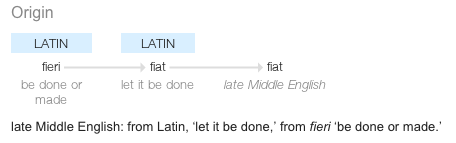
\includegraphics{assets/images/fiat-definition.png}
  \caption{fiat --- 'Let it be done'}
  \label{fig:fiat-definition}
\end{figure}

Until recently, two types of money were used: \textbf{commodity money}, made
out of precious \textit{things}, and \textbf{representative money}, which simply
\textit{represents} the precious thing, mostly in writing.

We already touched on commodity money above. People used special bones,
seashells, and precious metals as money. Later on, mainly coins made out
of precious metals like gold and silver were used as money. The [oldest
coin] found so far is made of a natural gold-and-silver mix and was made
more than 2700 years ago. If something is new in Bitcoin, the concept of
a coin is not it.

\begin{figure}
  \centering
  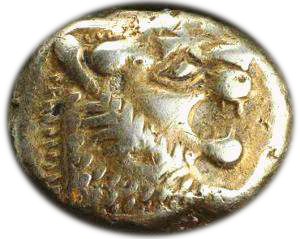
\includegraphics[width=5cm]{assets/images/lydian-coin-stater.png}
  \caption{Lydian electrum coin}
  \label{fig:lydian-coin-stater}
\end{figure}

Turns out that hoarding coins, or hodling, to use today's parlance, is
almost as old as coins. The earliest coin hodler was someone who put
almost a hundred of these coins in a pot and buried it in the
foundations of a temple, only to be found 2500 years later. Pretty good
cold storage if you ask me.

One of the downsides of using precious metal coins is that they can be
clipped, effectively debasing the value of the coin. New coins can be
minted from the clippings, inflating the money supply over time,
devaluing every individual coin in the process. People were literally
shaving off as much as they could get away with of their silver dollars.
I wonder what kind of \textit{Dollar Shave Club} advertisements they had back
in the day.

Since governments are only cool with inflation if they are the ones
doing it, efforts were made to stop this guerrilla debasement. In
classic cops-and-robbers fashion, coin clippers got ever more creative
with their techniques, forcing the 'masters of the mint' to get even
more creative with their countermeasures. Isaac Newton, the
world-renowned physicist of \textit{Principia Mathematica} fame, used to be one
of these masters. He is attributed with adding the small stripes at the
side of coins which are still present today. Gone were the days of easy
coin shaving.

\begin{figure}
  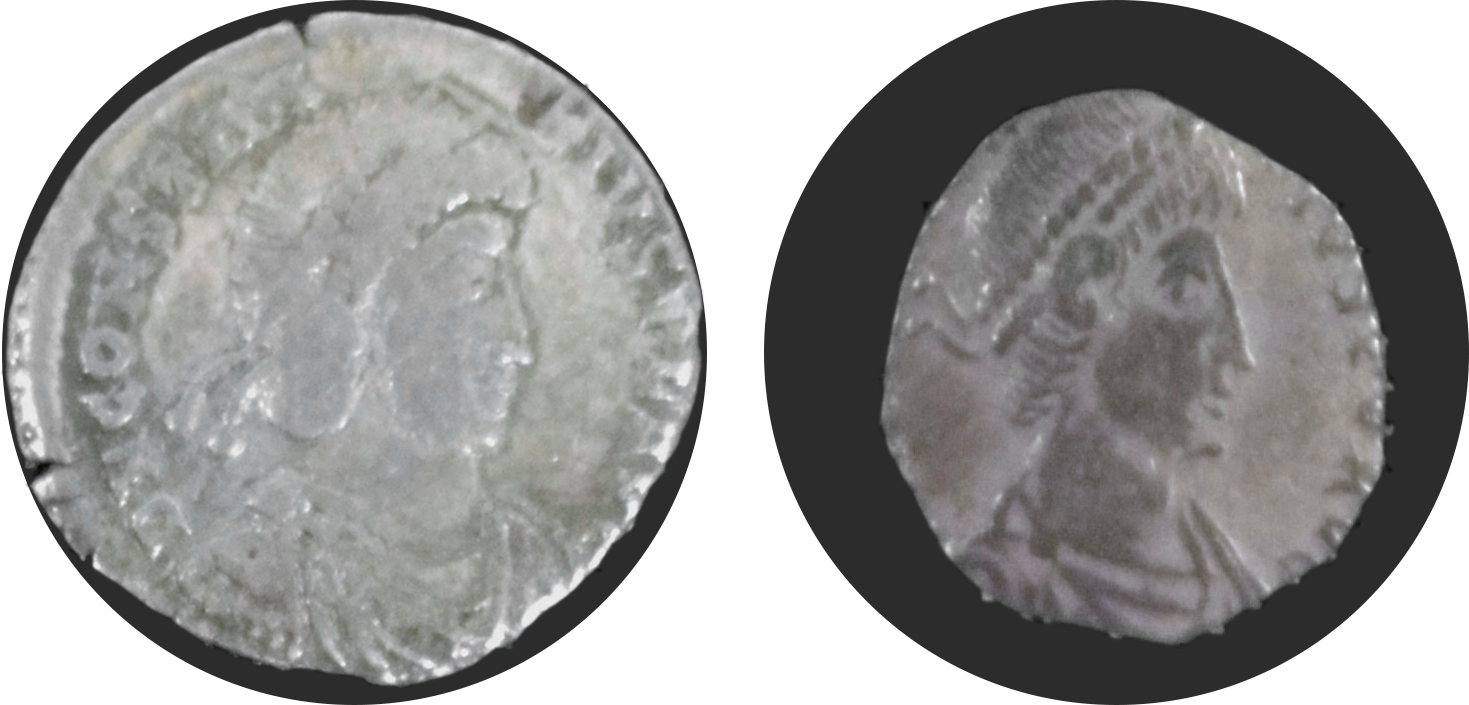
\includegraphics{assets/images/clipped-coins.png}
  \label{fig:clipped-coins}
\end{figure}

Even with these methods of [coin debasement] kept in check, coins still
suffer from other issues. They are bulky and not very convenient to
transport, especially when large transfers of value need to happen.
Showing up with a huge bag of silver dollars every time you want to buy
a Mercedes isn't very practical.

Speaking of German things: How the United States \textit{dollar} got its name
is another interesting story. The word "dollar" is derived from the
German word \textit{[Thaler]*, short for a *Joachimsthaler.} A Joachimsthaler
was a coin minted in the town of \textit{Sankt Joachimsthal}. Thaler is simply
a shorthand for someone (or something) coming from the valley, and
because Joachimsthal was \textit{the} valley for silver coin production, people
simply referred to these silver coins as \textit{Thaler.} Thaler (German)
morphed into daalders (Dutch), and finally dollars (English).

\begin{figure}
  \centering
  
\includegraphics[width=5cm]{assets/images/joachimsthaler.png}
  \caption{The original `dollar'. Saint Joachim is pictured with his robe and wizard hat. Picture cc-by-sa Wikipedia user Berlin-George}
  \label{fig:joachimsthaler}
\end{figure}

The introduction of representative money heralded the downfall of hard
money. Gold certificates were introduced in 1863, and about fifteen
years later, the silver dollar was also slowly but surely being replaced
by a paper proxy: the silver certificate.

It took about 50 years from the introduction of the first [silver
certificates] until these pieces of paper morphed into something that we
would today recognize as one U.S. dollar.

\begin{figure}
  \centering
  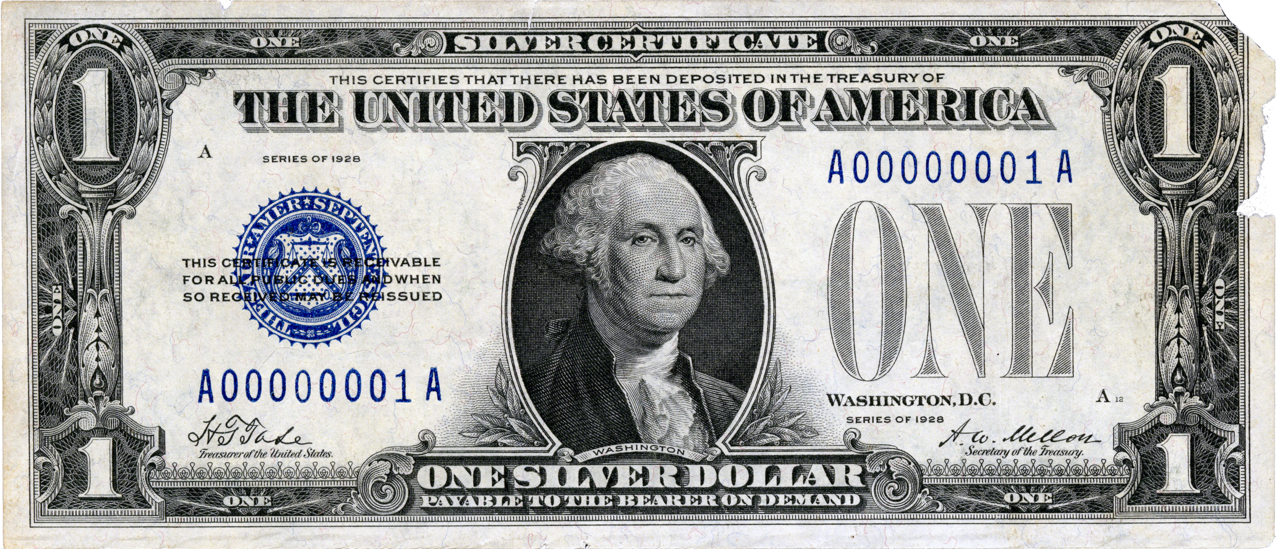
\includegraphics{assets/images/us-silver-dollar-note-smaller.png}
  \caption{A 1928 U.S. silver dollar. `Payable to the bearer on demand.' Picture credit to the National Numismatic Collection at the Smithsonian Institution}
  \label{fig:us-silver-dollar-note-smaller}
\end{figure}

Note that the 1928 U.S. silver dollar above still goes by the name of
\textit{silver certificate}, indicating that this is indeed simply a document
stating that the bearer of this piece of paper is owed a piece of
silver. It is interesting to see that the text which indicates this got
smaller over time. The trace of "certificate" vanished completely after
a while, being replaced by the reassuring statement that these are
federal reserve notes.

As mentioned above, the same thing happened to gold. Most of the world
was on a [bimetallic standard], meaning coins were made primarily of
gold and silver. Having certificates for gold, redeemable in gold coins,
was arguably a technological improvement. Paper is more convenient,
lighter, and since it can be divided arbitrarily by simply printing a
smaller number on it, it is easier to break into smaller units.

To remind the bearers (users) that these certificates were
representative for actual gold and silver, they were colored accordingly
and stated this clearly on the certificate itself. You can fluently read
the writing from top to bottom:

\begin{quotation}
``This certifies that there have been deposited in the treasury of the
United States of America one hundred dollars in gold coin payable to
the bearer on demand.''
\end{quotation}

\begin{figure}
  \centering
  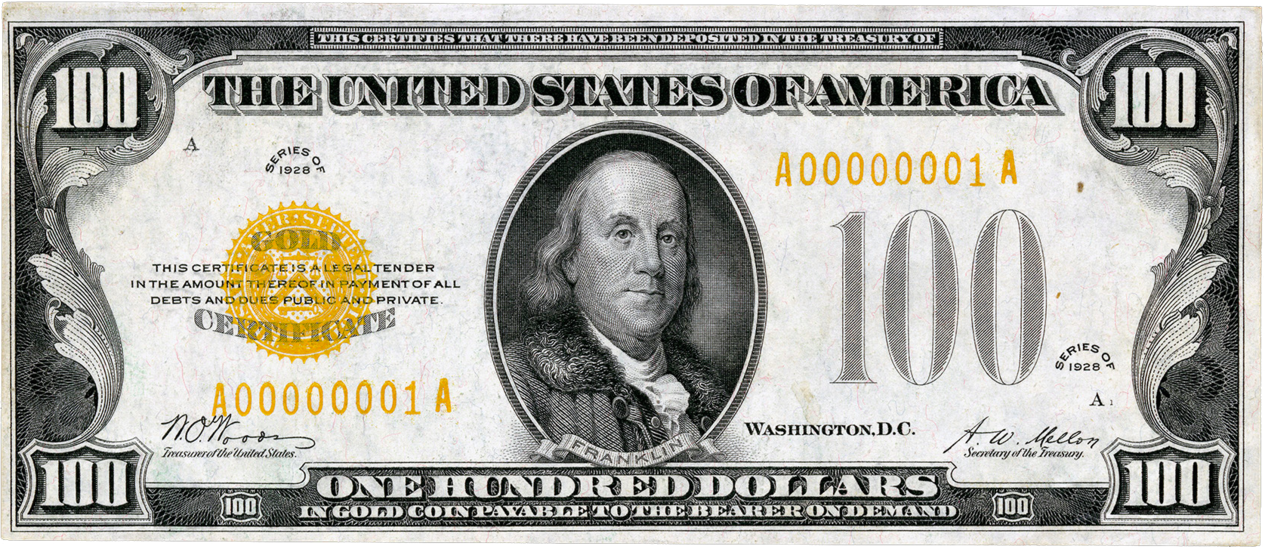
\includegraphics{assets/images/us-gold-cert-100-smaller.png}
  \caption{Picture credit to National Numismatic Collection, National Museum of American History.}
  \label{fig:us-gold-cert-100-smaller}
\end{figure}

In 1963, the words "PAYABLE TO THE BEARER ON DEMAND" were removed from
all newly issued notes. Five years later, the redemption of paper notes
for gold and silver ended.

The words hinting on the origins and the idea behind paper money were
removed. The golden color disappeared. All that was left was the paper
and with it the ability of the government to print as much of it as it
wishes.

With the abolishment of the gold standard in 1971, this century-long
sleight-of-hand was complete. Money became the illusion we all share to
this day: fiat money. It is worth something because someone commanding
an army and operating jails says it is worth something. As can be
clearly read on every dollar note in circulation today, "THIS NOTE IS
LEGAL TENDER". In other words: It is valuable because the note says so.

\begin{figure}
  \centering
  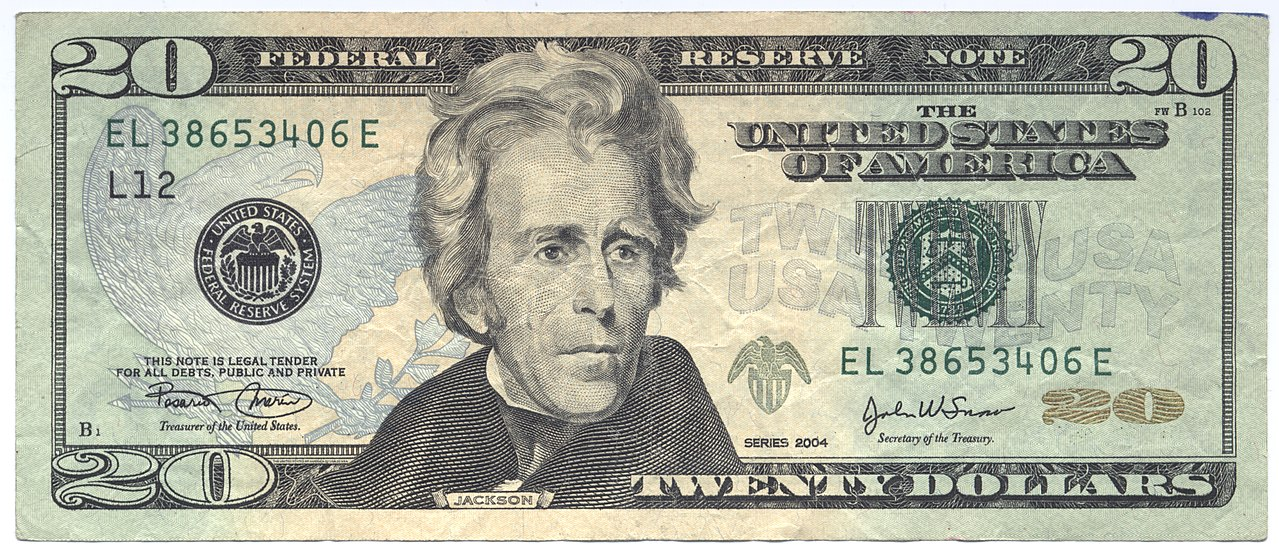
\includegraphics{assets/images/us-dollar-2004.jpg}
  \caption{A 2004 series U.S. twenty dollar note used today. `THIS NOTE IS LEGAL TENDER'}
  \label{fig:us-dollar-2004}
\end{figure}

By the way, there is another interesting lesson on today's bank notes,
hidden in plain sight. The second line reads that this is legal tender
"FOR ALL DEBTS, PUBLIC AND PRIVATE". What might be obvious to economists
was surprising to me: All money is debt. My head is still hurting
because of it, and I will leave the exploration of the relation of money
and debt as an exercise to the reader.

As we have seen, gold and silver were used as money for millennia. Over
time, coins made from gold and silver were replaced by paper. Paper
slowly became accepted as payment. This acceptance created an
illusion --- the illusion that the paper itself has value. The final
move was to completely sever the link between the representation and the
actual: abolishing the gold standard and convincing everyone that the
paper in itself is precious.

\paragraph{Bitcoin taught me about the history of money and the greatest sleight of
hand in the history of economics: fiat currency.}

% ---
%
% #### Down the Rabbit Hole
%
% - [Shelling Out: The Origins of Money] by Nick Szabo
% - [Methods of Coin Debasement][coin debasement], [Thaler], [U.S. Silver Certificate][silver certificates], [Bimetallism][bimetallic standard] on Wikipedia
%
% [oldest coin]: https://www.britishmuseum.org/explore/themes/money/the_origins_of_coinage.aspx
% [coin debasement]: https://en.wikipedia.org/wiki/Methods_of_coin_debasement
% [Thaler]: https://en.wikipedia.org/wiki/Thaler
% [Berlin-George]: https://en.wikipedia.org/wiki/File:Bohemia,_Joachimsthaler_1525_Electrotype_Copy._VF._Obverse..jpg
% [silver certificates]: https://en.wikipedia.org/wiki/Silver_certificate_%28United_States%29
% [bimetallic standard]: https://en.wikipedia.org/wiki/Bimetallism
% [Shelling Out: The Origins of Money]: https://nakamotoinstitute.org/shelling-out/
%
% <!-- Wikipedia -->
% [alice]: https://en.wikipedia.org/wiki/Alice%27s_Adventures_in_Wonderland
% [carroll]: https://en.wikipedia.org/wiki/Lewis_Carroll

% ---
layout: lesson
title: Lesson 13
categories: [bitcoin, lesson]
audio: /assets/audio/21lessons/2-13.m4a
---

\chapter{ Fractional Reserve Insanity}
\label{les:13}

\begin{chapquote}{Lewis Carroll, \textit{Alice in Wonderland}}
Alas! it was too late: she went on growing and growing, and very soon had to
kneel down: in another minute there was not room even for this, and she tried
the effect of lying down, with one elbow against the door, and the other arm
curled round her head. Still she went on growing, and as a last resource she put
one arm out of the window, and one foot up the chimney, and said to herself
``now I can do no more—what will become of me?''
\end{chapquote}

Value and money aren't trivial topics, especially in today's times. The
process of money creation in our banking system is equally non-trivial,
and I can't shake the feeling that this is deliberately so. What I have
previously only encountered in academia and legal texts seems to be
common practice in the financial world as well: nothing is explained in
simple terms, not because it is truly complex, but because the truth is
hidden behind layers and layers of jargon and *apparent* complexity.
"Expansionary monetary policy, quantitative easing, fiscal stimulus to
the economy." The audience nods along in agreement, hypnotized by the
fancy words.

Fractional reserve banking and quantitative easing are two of those
fancy words, obfuscating what is really happening by masking it as
complex and difficult to understand. If you would explain them to a
five-year-old, the insanity of both will become apparent quickly.

Godfrey Bloom, addressing the European Parliament during a [joint
debate], said it way better than I ever could:

\begin{quotation}
[...] you do not really understand the concept of banking. All the
banks are broke. Bank Santander, Deutsche Bank, Royal Bank of
Scotland --- they're all broke! And why are they broke? It isn't an
act of God. It isn't some sort of tsunami. They're broke because we
have a system called 'fractional reserve banking' which means that
banks can lend money that they don't actually have! It's a criminal
scandal and it's been going on for too long. [...]
We have counterfeiting --- sometimes called quantitative
easing --- but counterfeiting by any other name. The artificial
printing of money which, if any ordinary person did, they'd go to
prison for a very long time [...] and until we start sending
bankers --- and I include central bankers and politicians --- to
prison for this outrage it will continue.
\end{quotation}
% > <cite>[Godfrey Bloom][joint debate]</cite>

Let me repeat the most important part: banks can lend money that they
don't actually have.

Thanks to fractional reserve banking, a bank only has to keep a small
*fraction* of every dollar it gets. It's somewhere between 0 and 10%,
usually at the lower end, which makes things even worse.

Let's use a concrete example to better understand this crazy idea: A
fraction of 10\% will do the trick and we should be able to do all the
calculations in our head. Win-win. So, if you take \$100 to a
bank --- because you don't want to store it under your mattress --- they
only have to keep the agreed upon *fraction* of it. In our example that
would be \$10, because 10\% of \$100 is \$10. Easy, right?

So what do banks do with the rest of the money? What happens to your
\$90? They do what banks do, they lend it to other people. The result is
a [money multiplier] effect, which increases the money supply in the
economy enormously. Your initial deposit of \$100 will soon turn into
\$190. By lending a 90\% fraction of the newly created \$90, there will
soon be \$271 in the economy. And \$343.90 after that. The money supply
is recursively increasing, since banks are literally lending money they
don't have. Without a single Abracadabra, banks magically transform
\$100 into one thousand dollars or more. Turns out 10x is easy. It only
takes a couple of lending rounds.

\begin{figure}
  \centering
  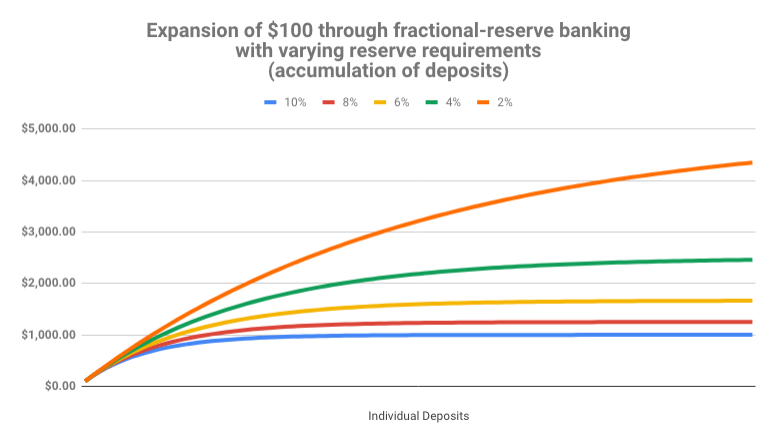
\includegraphics{assets/images/money-multiplier.png}
  % \caption{}
  \label{fig:money-multiplier}
\end{figure}

Don't get me wrong: There is nothing wrong with lending. There is
nothing wrong with interest. There isn't even anything wrong with good
old regular banks to store your wealth somewhere more secure than in
your sock drawer.

Central banks, however, are a different beast. Abominations of financial
regulation, half public half private, playing god with something which
affects everyone who is part of our global civilization, without a
conscience, only interested in the immediate future, and seemingly
without any accountability or [auditability].

While Bitcoin is still inflationary, it will cease to be so rather soon.
The strictly limited supply of 21 million bitcoins will eventually do
away with inflation completely. We now have two monetary worlds: an
inflationary one where money is printed arbitrarily, and the world of
Bitcoin, where final supply is fixed and easily auditable for everyone.
One is forced upon us by violence, the other can be joined by anyone who
wishes to do so. No barriers to entry, no one to ask for permission.
Voluntary participation. That is the beauty of Bitcoin.

I would argue that the argument between [Keynesian] and [Austrian]
economists is no longer purely academical. Satoshi managed to build a
system for value transfer on steroids, creating the soundest money which
ever existed in the process. One way or another, more and more people
will learn about the scam which is fractional reserve banking. If they
come to similar conclusions as most Austrians and Bitcoiners, they might
join the ever-growing internet of money. Nobody can stop them if they
choose to do so.

\paragraph{Bitcoin taught me that fractional reserve banking is pure insanity.}

% ---
%
% #### Down the Rabbit Hole
%
% - [The Creature From Jekyll Island] by G. Edward Griffin
% - [Why the whole banking system is a scam][joint debate] by Godfrey Bloom
% - [Money Multiplier][money multiplier], [Keynesian Economics][Keynesian], [Austrian School][Austrian] on Wikipedia
%
% [The Creature From Jekyll Island]: https://archive.org/details/pdfy--Pori1NL6fKm2SnY
%
% [joint debate]: https://www.youtube.com/watch?v=hYzX3YZoMrs
% [money multiplier]: https://en.wikipedia.org/wiki/Money_multiplier
% [auditability]: https://i.ytimg.com/vi/ThFGs347MW8/maxresdefault.jpg
% [Keynesian]: https://en.wikipedia.org/wiki/Keynesian_economics
% [Austrian]: https://en.wikipedia.org/wiki/Austrian_School
%
% <!-- Wikipedia -->
% [alice]: https://en.wikipedia.org/wiki/Alice%27s_Adventures_in_Wonderland
% [carroll]: https://en.wikipedia.org/wiki/Lewis_Carroll

% \chapter{ Sound Money}
\label{les:14}

\begin{chapquote}{Lewis Carroll, \textit{Alice in Wonderland}}
``The first thing I've got to do,'' said Alice to herself, as she wandered about
in the wood, ``is to grow to my right size, and the second thing is to find my
way into that lovely garden. I think that will be the best plan.''
\end{chapquote}

The most important lesson I have learned from Bitcoin is that in the
long run, hard money is superior to soft money. Hard money, also
referred to as *sound money*, is any globally traded currency that
serves as a reliable store of value.

Granted, Bitcoin is still young and volatile. Critics will say that it
does not store value reliably. The volatility argument is missing the
point. Volatility is to be expected. The market will take a while to
figure out the just price of this new money. Also, as is often jokingly
pointed out, it is grounded in an error of measurement. If you think in
dollars you will fail to see that one bitcoin will always be worth one
bitcoin.

\begin{quotation}
``A fixed money supply, or a supply altered only in accord with
objective and calculable criteria, is a necessary condition to a
meaningful just price of money.''
\end{quotation}
% > <cite>[Fr. Bernard W. Dempsey, S.J.]</cite>

As a quick stroll through the graveyard of forgotten currencies has
shown, money which can be printed will be printed. So far, no human in
history was able to resist this temptation.

Bitcoin does away with the temptation to print money in an ingenious
way. Satoshi was aware of our greed and fallibility --- this is why he
chose something more reliable than human restraint: mathematics.

\begin{figure}
  \centering
  \begin{equation}
  \sum\limits_{i=0}^{32} \frac{21000 \lfloor \frac{50*10^8}{2^i} \rfloor}{10^8}
  \end{equation}
  \caption{Bitcoin's supply formula}
  \label{fig:supply-formula-white}
\end{figure}

While this formula is useful to describe Bitcoin's supply, it is
actually nowhere to be found in the code. Issuance of new bitcoin is
done in an [algorithmically controlled] fashion, by reducing the reward
which is paid to miners every four years. The formula above is used to
quickly sum up what is happening under the hood. What really happens can
be best seen by looking at the change in block reward, the reward paid
out to whoever finds a valid block, which roughly happens every 10
minutes.


\begin{figure}
  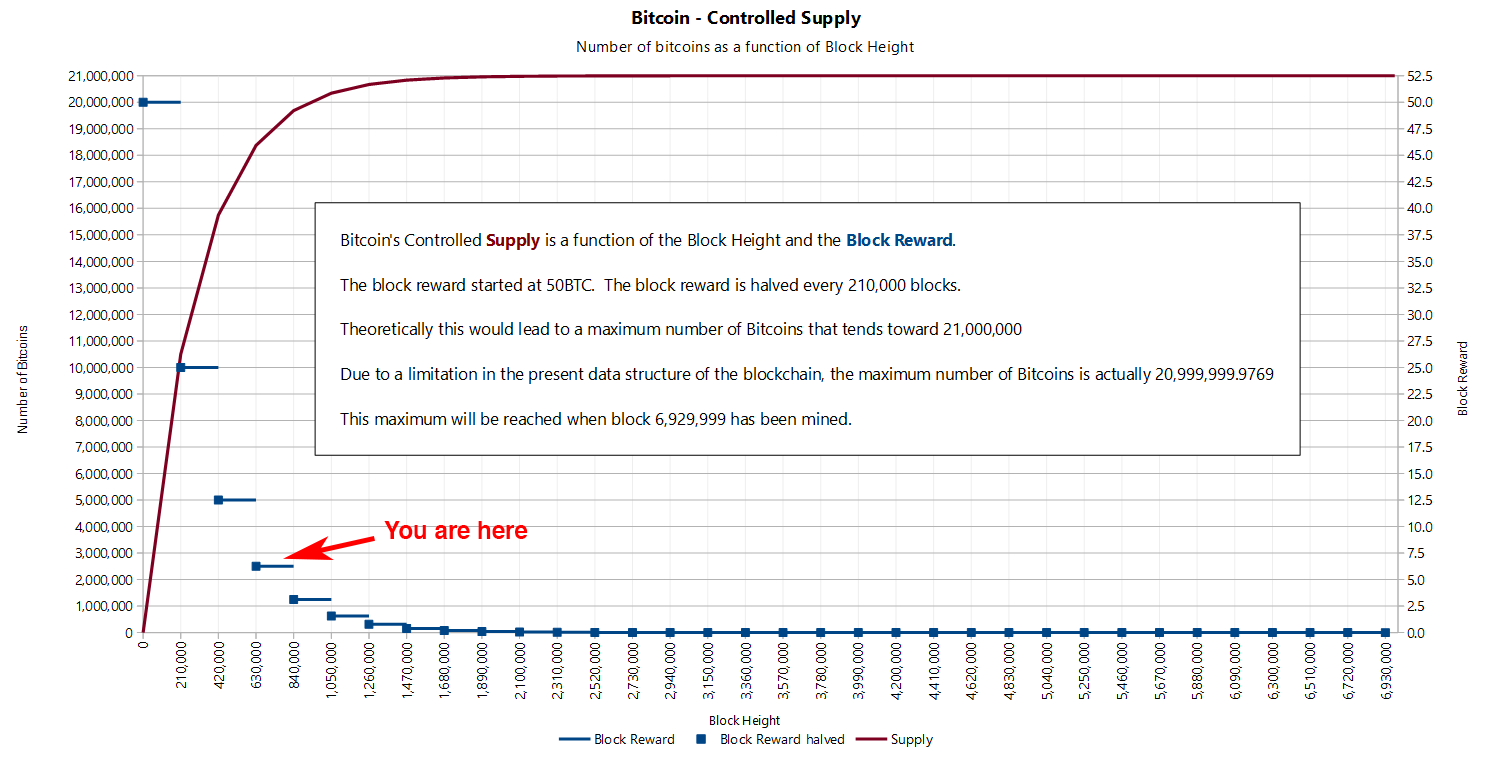
\includegraphics{assets/images/you-are-here.png}
  \caption{Bitcoin's controlled supply}
  \label{fig:you-are-here.png}
\end{figure}

Formulas, logarithmic functions and exponentials are not exactly
intuitive to understand. The concept of *soundness* might be easier to
understand if looked at in another way. Once we know how much there is
of something, and once we know how hard this something is to produce or
get our hands on, we immediately understand its value. What is true for
Picasso's paintings, Elvis Presley's guitars, and Stradivarius violins
is also true for fiat currency, gold, and bitcoins.

The hardness of fiat currency depends on who is in charge of the
respective printing presses. Some governments might be more willing to
print large amounts of currency than others, resulting in a weaker
currency. Other governments might be more restrictive in their money
printing, resulting in harder currency.

Before we had fiat currencies, the soundness of money was determined by
the natural properties of the stuff which we used as money. The amount
of gold on earth is limited by the laws of physics. Gold is rare because
supernovae and neutron star collisions are rare. The "flow" of gold is
limited because extracting it is quite an effort. Being a heavy element
it is mostly buried deep underground.

The abolishment of the gold standard gave way to a new reality: adding
new money requires just a drop of ink. In our modern world adding a
couple of zeros to the balance of a bank account requires even less
effort: flipping a few bits in a bank computer is enough.

\begin{quotation}
``One important aspect of this new reality is that institutions like
the Fed cannot go bankrupt. They can print any amount of money that
they might need for themselves at virtually zero cost.''
\end{quotation}
% <cite>[Jörg Guido Hülsmann]</cite>

The principle outlined above can be expressed more generally as the
ratio of "stock" to "flow". Simply put, the *stock* is how much of
something is currently there. For our purposes, the stock is a measure
of the current money supply. The *flow* is how much there is produced
over a period of time (e.g. per year). The key to understanding sound
money is in understanding this stock-to-flow ratio.

Calculating the stock-to-flow ratio for fiat currency is difficult,
because [how much money there is] depends on how you look at it. You
could count only banknotes and coins (M0), add traveler checks and check
deposits (M1), add saving accounts and mutual funds and some other
things (M2), and even add certificates of deposit to all of that (M3).
Further, how all of this is defined and measured varies from country to
country and since the US Federal Reserve [stopped publishing] numbers
for M3, we will have to make do with the M2 monetary supply. I would
love to verify these numbers, but I guess we have to trust the fed for
now.

Gold, one of the rarest metals on earth, has the highest stock-to-flow
ratio. According to the US Geological Survey, a little more than 190,000
tons have been mined. In the [last few years], around 3100 tons of gold
have been mined per year.

Using these numbers, we can easily calculate the stock-to-flow ratio for
gold:

\begin{figure}
  \centering
  \begin{equation}
  \frac{190,000 tons}{3,100 tons} = ~ 61
  \end{equation}
  \caption{Stock-to-flow ratio of gold}
  \label{fig:stock-to-flow-gold}
\end{figure}

Nothing has a higher stock-to-flow ratio than gold. This is why gold, up
to now, was the hardest, soundest money in existence. It is often said
that all the gold mined so far would fit in two olympic-sized swimming
pools. According to [my calculations], we would need four. So maybe this
needs updating, or Olympic-sized swimming pools got smaller.

Enter Bitcoin. As you probably know, bitcoin mining was all the rage in
the last couple of years. This is because we are still in the early
phases of what is called the *reward era*, where mining nodes are
rewarded with *a lot* of bitcoin for their computational effort. We are
currently in reward era number 3, which began in 2016 and will end in
early 2020, probably in May. While the bitcoin supply is predetermined,
the inner workings of Bitcoin only allow for approximate dates.
Nevertheless, we can predict with certainty how high Bitcoin's
stock-to-flow ratio will be. Spoiler alert: it will be high.

How high? Well, it turns out that Bitcoin will get infinitely hard.

\begin{figure}
  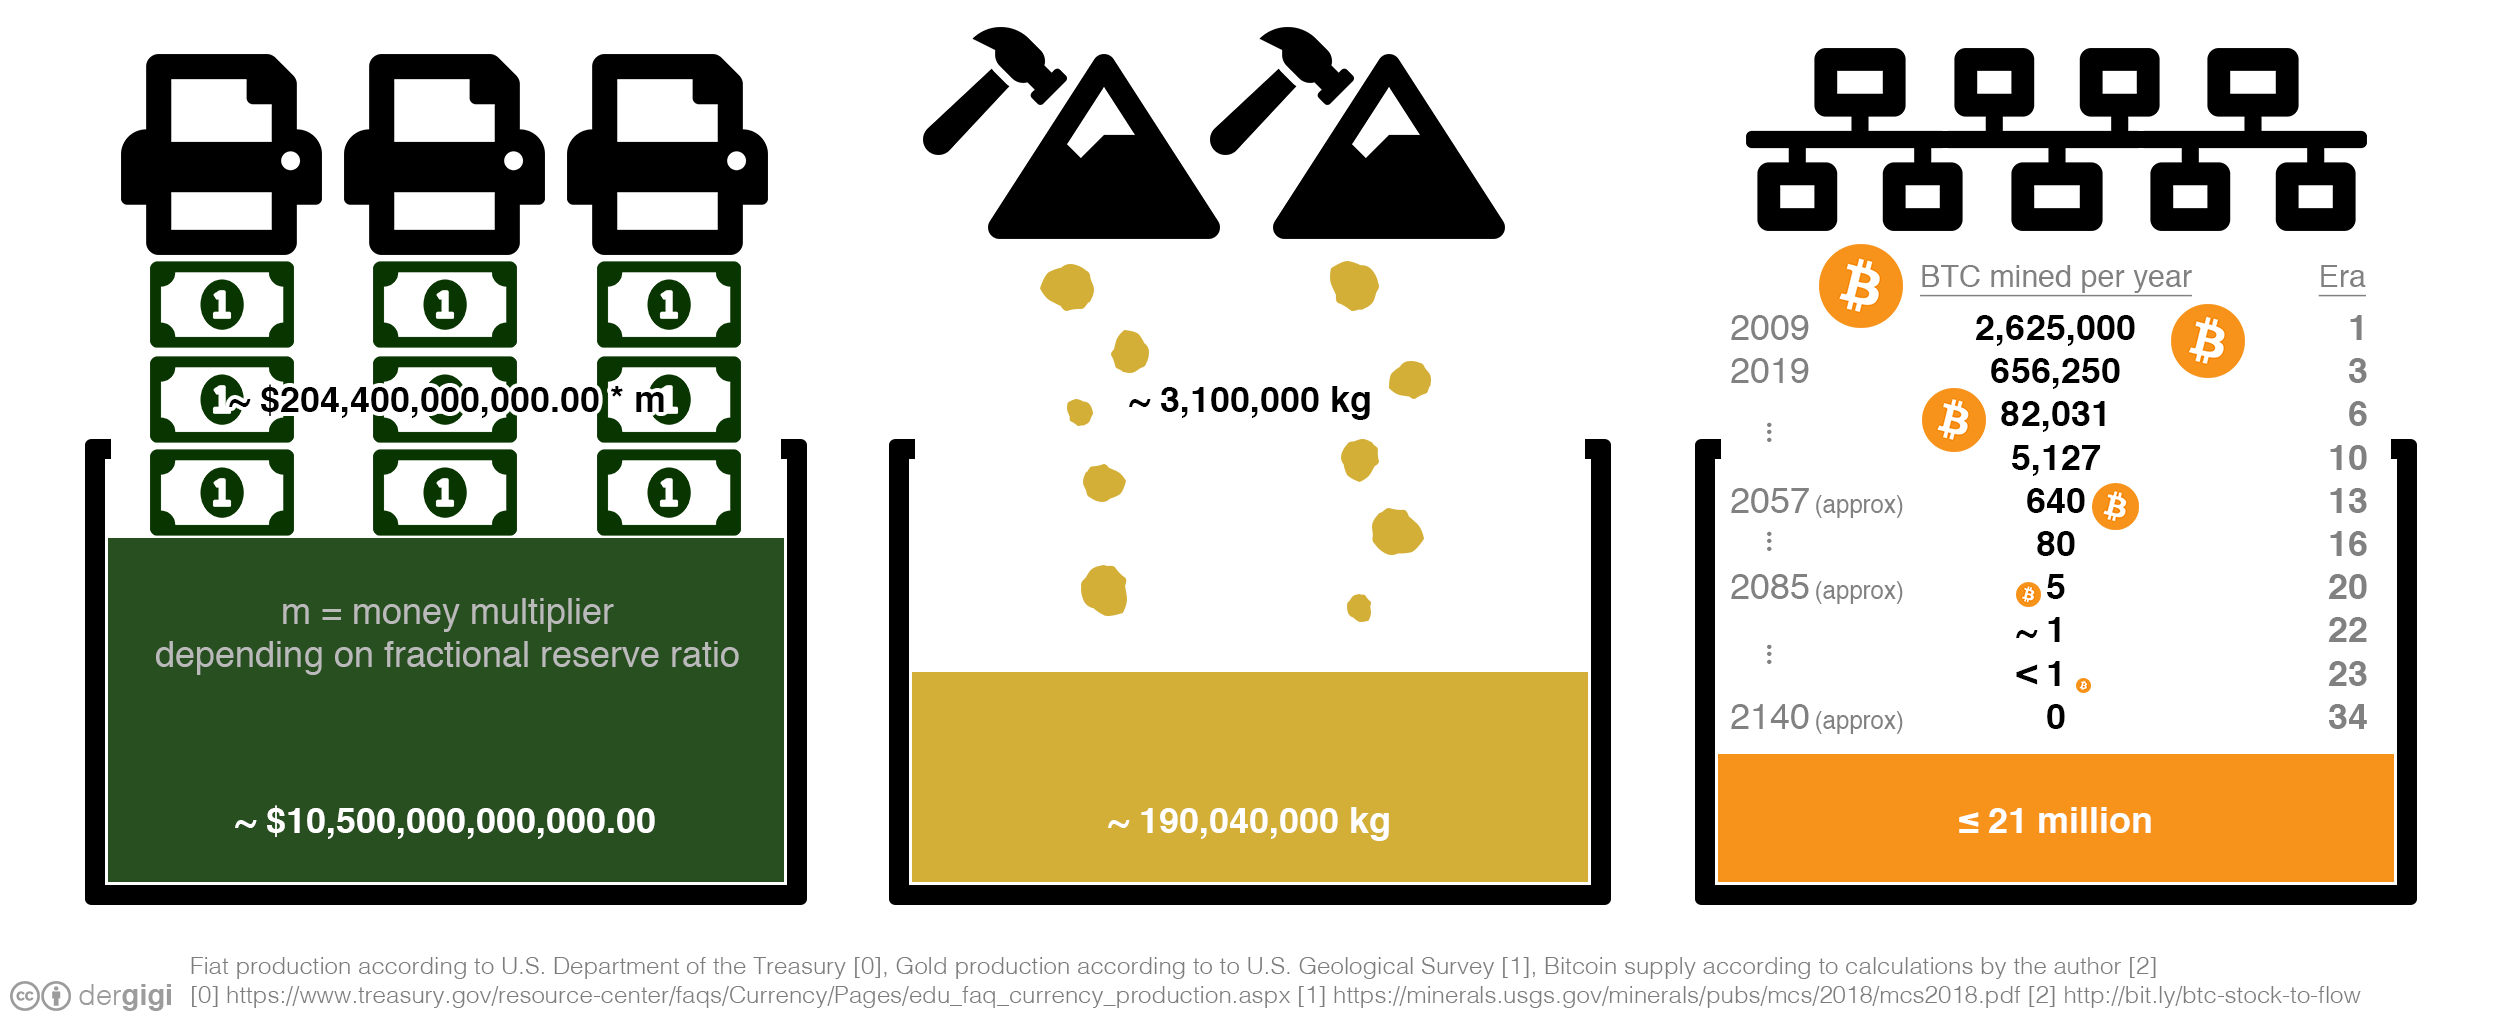
\includegraphics{assets/images/stock-to-flow-white-cc-by-sources.png}
  \caption{Visualization of stock and flow for USD, gold, and Bitcoin}
  \label{fig:stock-to-flow-white-cc-by-sources}
\end{figure}

Due to an exponential decrease of the mining reward, the flow of new
bitcoin will diminish resulting in a sky-rocketing stock-to-flow ratio.
It will catch up to gold in 2020, only to surpass it four years later by
doubling its soundness again. Such a doubling will occur 64 times in
total. Thanks to the power of exponentials, the number of bitcoin mined
per year will drop below 100 bitcoin in 50 years and below 1 bitcoin in
75 years. The global faucet which is the block reward will dry up
somewhere around the year 2140, effectively stopping the production of
bitcoin. This is a long game. If you are reading this, you are still
early.

\begin{figure}
  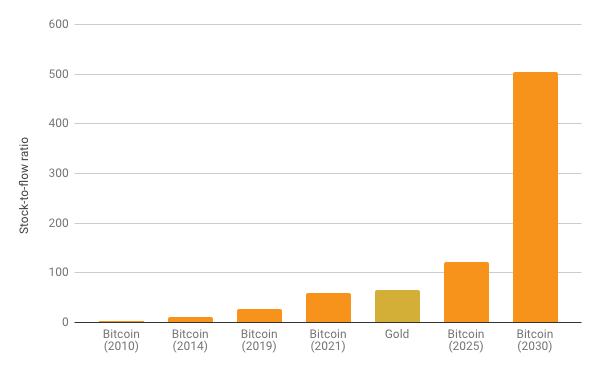
\includegraphics{assets/images/soundness-over-time.png}
  \caption{Rising stock-to-flow ratio of bitcoin as compared to gold}
  \label{fig:soundness-over-time}
\end{figure}

As bitcoin approaches infinite stock to flow ratio it will be the
soundest money in existence. Infinite soundness is hard to beat.

Viewed through the lens of economics, Bitcoin's *difficulty adjustment*
is probably its most important component. How hard it is to mine bitcoin
depends on how quickly new bitcoins are mined\*. It is the dynamic
adjustment of the network's mining difficulty which enables us to
predict its future supply.

*(\* It actually depends on how quickly valid blocks are found, but for
our purposes, this is the same thing as "mining bitcoins" and will be so
for the next 120 years.)*

The simplicity of the difficulty adjustment algorithm might distract
from its profundity, but the difficulty adjustment truly is a revolution
of Einsteinian proportions. It ensures that, no matter how much or how
little effort is spent on mining, Bitcoin's controlled supply won't be
disrupted. As opposed to every other resource, no matter how [much
energy] someone will put into mining bitcoin, the total reward will not
increase.

Just like $E=mc^2$ dictates the [universal speed limit] in our universe,
Bitcoin's difficulty adjustment dictates the **universal money limit**
in Bitcoin.

If it weren't for this difficulty adjustment, all bitcoins would have
been mined already. If it weren't for this difficulty adjustment,
Bitcoin probably wouldn't have survived in its infancy. It is what
secures the network in its reward era. It is what ensures a steady and
[fair distribution] of new bitcoin. It is the thermostat which regulates
Bitcoin's monetary policy.

Einstein showed us something novel: no matter how hard you push an
object, at a certain point you won't be able to get more speed out of
it. Satoshi also showed us something novel: no matter how hard you dig
for this digital gold, at a certain point you won't be able to get more
bitcoin out of it. For the first time in human history, we have a
monetary good which, no matter how hard you try, you won't be able to
produce more of.

Bitcoin taught me that sound money is essential.

% ---
%
% #### Through the Looking-Glass
%
% - [Bitcoin's Energy Consumption: A Shift in Perspective][much energy]
%
% #### Down the Rabbit Hole
%
% - [The Ethics of Money Production][Jörg Guido Hülsmann] by Jörg Guido Hülsmann
% - [Mineral Commodity Summaries 2019][last few years] by the United States Geological Survey
% - [Bitcoin’s Distribution was Fair][fair distribution] by Dan Held
% - [Bitcoin's Controlled Supply][algorithmically controlled] on the Bitcoin Wiki
% - [Money Supply][how much money there is], [Speed of Light][universal speed limit] on Wikipedia
%
% <!-- Internal -->
% [much energy]: 
%
% [Fr. Bernard W. Dempsey, S.J.]: https://www.jstor.org/stable/29769582
% [Jörg Guido Hülsmann]: https://mises.org/sites/default/files/The%20Ethics%20of%20Money%20Production_2.pdf
% [stopped publishing]: https://www.federalreserve.gov/Releases/h6/discm3.htm
% [last few years]: https://minerals.usgs.gov/minerals/pubs/mcs/2018/mcs2018.pdf
% [my calculations]: https://www.wolframalpha.com/input/?i=volume+of+190000+metric+tons+gold+%2F+olympic+swimming+pool+volume
% [fair distribution]: https://blog.picks.co/bitcoins-distribution-was-fair-e2ef7bbbc892
%
% <!-- Bitcoin Wiki -->
% [algorithmically controlled]: https://en.bitcoin.it/wiki/Controlled_supply
%
% <!-- Wikipedia -->
% [how much money there is]: https://en.wikipedia.org/wiki/Money_supply
% [universal speed limit]: https://en.wikipedia.org/wiki/Speed_of_light#Upper_limit_on_speeds
% [alice]: https://en.wikipedia.org/wiki/Alice%27s_Adventures_in_Wonderland
% [carroll]: https://en.wikipedia.org/wiki/Lewis_Carroll

% \part{Technology}
\label{ch:technology}

\begin{chapquote}{Lewis Carroll, \textit{Alice in Wonderland}}
``Now, I'll manage better this time'' she said to herself, and began by taking
the little golden key, and unlocking the door that led into the garden
\end{chapquote}

\textit{Golden keys}, clocks which only work by chance, races to solve
strange riddles, and builders that don't have faces or names. What sounds like
fairy tales from Wonderland is daily business in the world of Bitcoin.

As we explored in [Chapter 2][chapter2], large parts of the current financial
system are systematically broken. Like Alice, we can only hope to manage better
this time. But, thanks to a pseudonymous inventor, we have incredibly
sophisticated technology to support us this time around: Bitcoin.

Solving problems in a radically decentralized and adversarial environment
requires unique solutions. What would otherwise be trivial problems to solve
are everything but in this strange world of nodes. Bitcoin relies on strong
cryptography for most solutions, at least if looked at through the lens of
technology. Just how strong this cryptography is will be explored in one of the
following lessons.

\textit{Cryptography} is what Bitcoin uses to remove trust in authorities.
Instead of relying on centralized institutions, the system relies on the final
authority of our universe: physics. Some grains of trust still remain, however.
We will examine these grains in the second lesson of this chapter.

~

Part III -- Technology:

\begin{enumerate}
  \item Strength in numbers
  \item Reflections on \enquote{Don't Trust, Verify}
  \item Telling time takes work
  \item Move slowly and don't break things
  \item Privacy is not dead
  \item Cypherpunks write code
  \item Metaphors for Bitcoin's future
\end{enumerate}

The last couple of lessons explore the ethos of technological development in
Bitcoin, which is arguably as important as the technology itself. Bitcoin is not
the next shiny app on your phone. It is the foundation of a new economic
reality, which is why Bitcoin should be treated as nuclear-grade financial
software.

Where are we in this financial, societal, and technological revolution? Networks
and technologies of the past may serve as metaphors for Bitcoins future, which
are explored in the last lesson of this chapter.

Once more, strap in and enjoy the ride. Like all exponential technologies, we
are about to go parabolic.

% \chapter{Stärke in Zahlen}
\label{les:15}

\begin{chapquote}{Lewis Carroll, \textit{Alice im Wunderland}}
\enquote{Mal sehen: Viermal fünf ist zwölf, und viermal sechs ist dreizehn, und
viermal sieben ist vierzehn – oh je! Auf diese Weise komme ich ja nie bis
Zwanzig!}
\end{chapquote}

Zahlen sind ein wesentlicher Bestandteil unseres alltäglichen Lebens. Die
meisten von uns sind jedoch nicht recht gut mit großen Zahlen vertraut. Die
größten Zahlen denen wir im täglichen Leben begegnen, liegen in der
Größenordnung von Millionen, Milliarden oder Billionen. Wir können über
Millionen von Menschen in Armut oder Milliarden von Dollar die für die
Rettungsschirme für Banken ausgegeben werden oder gar über Trillionen von
Staatsschulden lesen. Auch wenn es schwer ist diese Schlagzeilen zu
interpretieren, können wir Zahlen dieser Größenordnung gewissermaßen einordnen.

Obwohl wir mit Milliarden und Billionen noch etwas anfangen können, beginnt
unsere Intuition bereits bei Zahlen der Größenordnung Milliarden zu versagen.
Hast du eine Ahnung, wie lange du warten müsstest bis eine Million / Milliarden
/ Billionen Sekunden vergehen? Wenn du nur ein bisschen wie ich bist, wärst du
jetzt verloren ohne die Zahlen genauer runterzubrechen.

Betrachten wir das Beispiel: Der Unterschied ist eine Erhöhung um drei
Zehnerpotenzen: $10^6$, $10^9$, $10^{12}$. In Sekunden zu denken bringt uns
nicht weiter also lass uns das in etwas übersetzen das wir verstehen:

\begin{itemize}
  \item $10^6$: Eine Million Sekunden war vor $1 1/2$ Wochen.
  \item $10^9$: Eine Milliarde Sekunden war vor fast 32 Jahren.
  \item $10^{12}$: Vor einer Billion Sekunden war Manhattan noch von einer
  dicken Eisschicht bedeckt.\footnote{Eine Billion Sekunden ($10^{12}$)
  entspricht $31.710$ Jahren. Das letzte Glazial setzte vor etwa 115.000 Jahren
  ein und endete vor etwa 11.700 Jahren.~\cite{wiki:LGM}}
\end{itemize}

\begin{figure}
  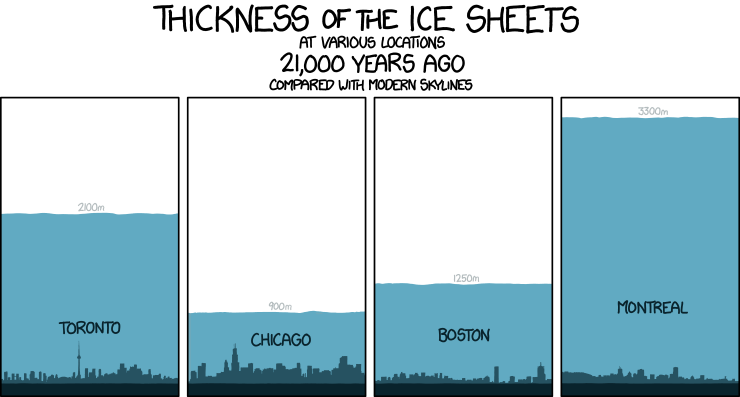
\includegraphics{assets/images/xkcd-1225.png}
  \caption{Dicke der Eisschichten vor ungefähr einer Billion Sekunden. Quelle: xkcd 1225}
  \label{fig:xkcd-1225}
\end{figure}

Sobald wir in den Bereich der modernen Kryptographie eintreten, versagt unsere
Intuition katastrophal. Bitcoin wurde um große Zahlen herum aufgebaut. Alles mit
der Tatsache, dass es praktisch unmöglich ist diese zu erraten. Die Zahlen sind
weitaus größer als alles was uns im Alltag begegnen könnte. Viele Zehnerpotenzen
größer. Zu verstehen wie groß diese Zahlen wirklich sind, ist entscheidend für
das Verständnis von Bitcoin als großem Ganzen.

Nehmen wir SHA-256\footnote{SHA-256 ist Teil von SHA-2, eine Gruppe von
verschiedenen kryptologischen Hashfunktionen welche von der NSA entwickelt
wurde.~\cite{wiki:sha2}}, eine der in Bitcoin verwendeten
Hashfunktionen\footnote{Bitcoin verwendet SHA-256 als
Block-Hashing-Algorithmus.~\cite{btcwiki:block-hashing}} als konkretes Beispiel.
Es liegt in der Natur der Sache, bei 256 Bits an
\enquote{Zweihundertsechsundfünzig} zu denken, was an sich ja keine große Zahl
ist. Die Zahl in SHA-256 spricht jedoch von Potenzen -- etwas womit unser Gehirn
eben nicht sonderlich gut klar kommt.

Während die Länge der Bits eine bequeme Metrik ist, geht die wahre Bedeutung der
256-Bit-Sicherheit bei der Übersetzung verloren. Ähnlich wie bei den oben
genannten Millionen ($10^6$) und Milliarden ($10^9$) spricht die Zahl in SHA-256
von Größenordnungen ($2^{256}$).

Also, wie stark ist SHA-256 genau?

\begin{quotation}\begin{samepage}
\enquote{SHA-256 ist sehr stark. Es ist nicht wie der nächste Schritt von MD5 zu
SHA1. Es kann mehrere Jahrzehnte andauern, es sei denn es gibt einen massiven
technologischen Durchbruch.}
\begin{flushright} -- Satoshi Nakamoto\footnote{Satoshi Nakamoto, in einer
Antwort zu Fragen über SHA-256 Kollisionen. \cite{satoshi-sha256}}
\end{flushright}\end{samepage}\end{quotation}

Ausgeschrieben ergibt $2^{256}$ folgende Zahl:

\begin{quotation}\begin{samepage}
    11 Duodezilliarden 579 Duodezillionen 289 Undezilliarden 237 Undezillionen
    316 Dezilliarden 195 Dezillionen 423 Nonilliarden 570 Nonillionen 985
    Oktilliarden 8 Oktillionen 687 Septilliarden 907 Septillionen 853
    Sextilliarden 269 Sextillionen 984 Quintilliarden 665 Quintillionen 640
    Quadrilliarden 564 Quadrillionen 39 Trilliarden 457 Trillionen 584
    Billiarden 7 Billionen 913 Milliarden 129 Millionen 639 Tausend 936.
\end{samepage}\end{quotation}

Das sind viele Nonilliarden! Es ist unmöglich diese Zahl zu verstehen. Es gibt
nichts im physikalischen Universum womit man sie vergleichen könnte. Sie ist
weitaus größer als die Anzahl aller Atome im beobachtbaren Universum. Das
menschliche Gehirn ist einfach nicht dafür geeignet schlau daraus zu werden.

Eine der besten Visualisierungen der wahren Stärke von SHA-256 ist das folgende
Video von Grant Sanderson. Mit dem treffenden Namen \textit{\enquote{Wie sicher
ist 256-Bit-Sicherheit?}}\footnote{\url{https://youtu.be/S9JGmA5_unY}} Tu dir
selbst den Gefallen und nimm dir die fünf Minuten Zeit um es dir anzusehen. Wie
alle anderen 3Blue1Brown Videos ist es nicht nur faszinierend, sondern auch
außergewöhnlich gut gemacht. Warnung: Du könntest in einen Mathe-Kaninchenbau
fallen.

\begin{figure}
  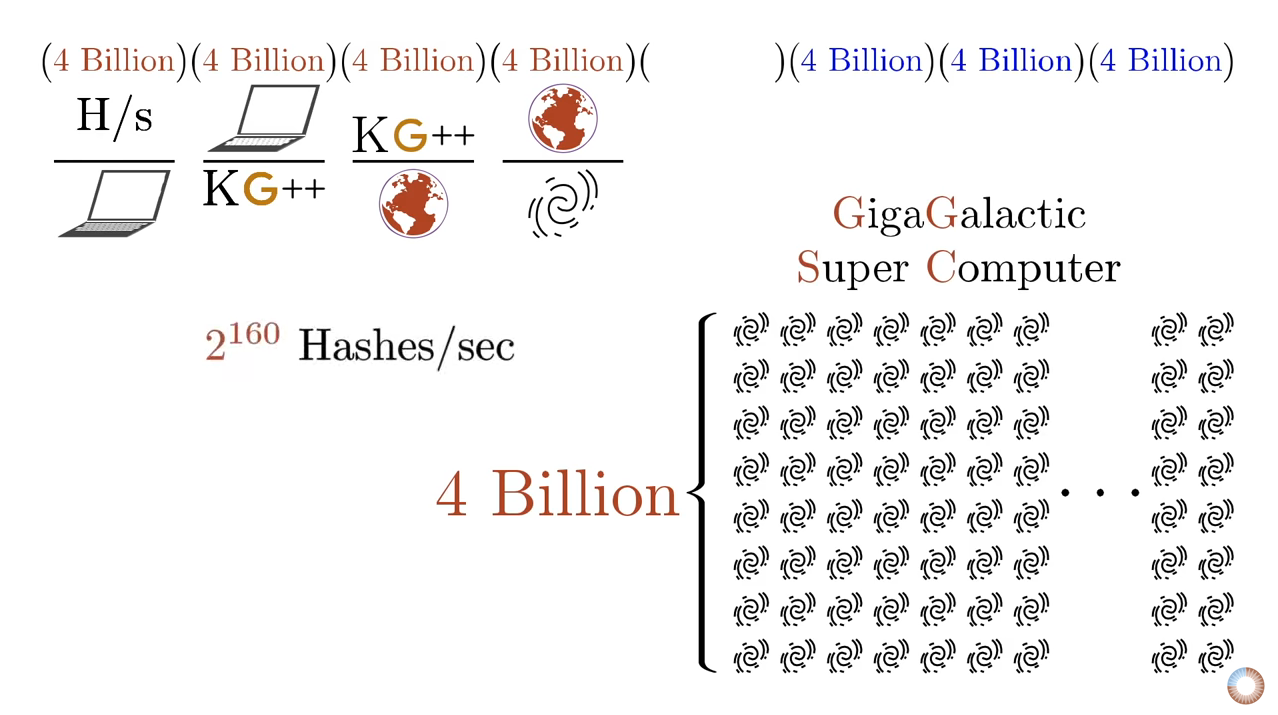
\includegraphics{assets/images/youtube-vid-inverted.png}
  \caption{Illustration von den Sicherheitsgarantien von SHA-256. Grafik aus dem Video von Grant Sanderson / 3Blue1Brown.}
  \label{fig:youtube-vid-inverted}
\end{figure}

Bruce Schneier~\cite{web:schneier} nutzte die physikalischen Grenzen der
Rechenleistung von heutigen Computern um diese Zahl zu beschreiben: Selbst wenn
wir einen optimalen Computer bauen könnten, welcher jede verfügbare Energie
nutzen würde um Bits perfekt zu manipulieren~\cite{wiki:landauer}, eine
Dyson-Sphäre\footnote{Eine Dyson-Sphäre, benannt nach Freeman Dyson, ist ein
hypothetisches Konstrukt, welches die Energie eines Sterns absorbiert oder
umlenkt, um sie somit optimal nutzen zu können.~\cite{wiki:dyson}} um unsere
Sonne herum bauen und sie 100 Milliarden Milliarden Jahre lang laufen lassen
würden, hätten wir immer noch nur eine Chance von $25\%$ eine Nadel in einem
256-Bit-Heuhaufen zu finden.

\begin{quotation}\begin{samepage}
\enquote{Diese Zahlen haben nichts mit der Technologie der Geräte zu tun; sie
sind die Maxima, die die Thermodynamik zulässt. Und sie implizieren stark, dass
Brute-Force-Angriffe auf 256-Bit-Schlüssel nicht möglich sind, bis Computer aus
etwas anderem als Materie gebaut werden und etwas anderes als Raum belegen.}
\begin{flushright} -- Bruce Schneier\footnote{Bruce Schneier, \textit{Applied Cryptography} \cite{bruce-schneier}}
\end{flushright}\end{samepage}\end{quotation}

Es ist schwer die Tiefgängikeit davon zu verdeutlichen. Starke Kryptographie
kehrt das Machtgleichgewicht der physischen Welt, an die wir so gewöhnt sind,
um. Dinge die man nicht knacken kann gibt es in der realen Welt nicht. Wende
genug Kraft auf und du kannst jede Tür, Box oder Schatzkiste öffnen.

Die Schatzkiste von Bitcoin ist ganz anders. Sie wird durch eine starke
Kryptographie gesichert, die Brute-Force Angriffen nur wenige Chancen bietet.
Und solange die zugrunde liegenden mathematischen Annahmen Bestand haben, sind
Brute-Force Attacken alles was wir in unserem Arsenal haben. Zugegeben, es gibt
auch die Option eines globalen \$5-Schraubenschlüsselangriffs (siehe
Abbildung~\ref{fig:xkcd-538}). Aber Folter wird nicht bei allen Bitcoin-Adressen
funktionieren und die kryptographischen Wände Bitcoins werden weiterhin
Brute-Force-Angriffe abwehren. Selbst wenn du es mit der Kraft von tausend
Sonnen versuchst. Wortwörtlich.

\begin{figure}
  \centering
  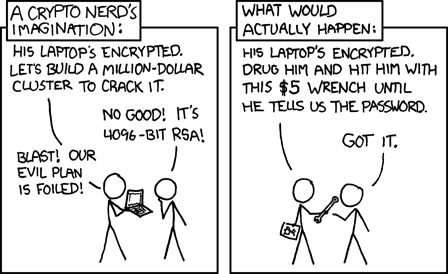
\includegraphics[width=8cm]{assets/images/xkcd-538.png}
  \caption{\$5-Schraubenschlüsselangriffs. Quelle: xkcd 538}
  \label{fig:xkcd-538}
\end{figure}

Diese Tatsache und ihre Auswirkungen wurden in dem \enquote{Call to
Cryptographic Arms} (\enquote{Aufruf zu kryptographischen Waffen}) treffend
zusammengefasst: \textit{\enquote{Keine Menge an Zwang oder Gewalt wird jemals ein
mathematisches Problem lösen.}}

\begin{quotation}\begin{samepage}
\enquote{Es ist nicht offensichtlich, dass die Welt auf diese Weise
funktionieren musste. Aber irgendwie lächelt das Universum in Bezug auf
Verschlüsselung.}
\begin{flushright} -- Julian Assange\footnote{Julian Assange, \textit{A Call to Cryptographic Arms} \cite{call-to-cryptographic-arms}}
\end{flushright}\end{samepage}\end{quotation}

Noch weiß niemand genau ob das Lächeln des Universums echt ist oder nicht. Es
ist möglich, dass unsere Annahme von mathematischen Asymmetrien falsch sind und
wir feststellen, dass P tatsächlich gleich NP \cite{wiki:pnp} ist oder wir
finden überraschender Weise schnelle Lösungen für spezifische Probleme
\cite{wiki:discrete-log} von denen wir derzeit annehmen, dass sie sehr schwer
oder gar unmöglich lösbar sind. Sollte dies der Fall sein wird die
Kryptographie, wie wir sie kennen, nicht mehr existieren und die Auswirkungen
würden höchstwahrscheinlich die Welt bis zur Unkenntlichkeit verändern.

\begin{quotation}\begin{samepage}
\enquote{Vires in Numeris} = \enquote{Stärke in Zahlen}\footnote{\textit{Vires
in Numeris} wurde das erste Mal von BitcoinTalk-User \textit{epii} als
Bitcoin-Motto vorgeschlagen.~\cite{epii}}
\end{samepage}\end{quotation}

\textit{Vires in numeris} ist nicht nur ein einprägsames Motto der Bitcoiner.
Die Erkenntnis, dass es eine unergründliche Kraft gibt die in Zahlen zu finden
ist, ist tiefgründig. Das und die Umkehrung der bestehenden Machtverhältnisse zu
verstehen, veränderte meine Sicht auf die Welt und die Zukunft die vor uns
liegt.

Ein direktes Resultat dessen ist die Tatsache, dass man niemanden um Erlaubnis
bitten muss um an Bitcoin teilzunehmen. Es gibt keine Seite auf der man sich
anmelden kann, kein verantwortliches Unternehmen, keine Regierungsbehörde an die
man Antragsformulare senden muss. Erstelle dir einfach eine große Zahl und du
kannst direkt loslegen. Die zentrale Behörde für die Kontoerstellung ist die
Mathematik. Und nur Gott weiß, wer dafür verantwortlich ist.

\begin{figure}
  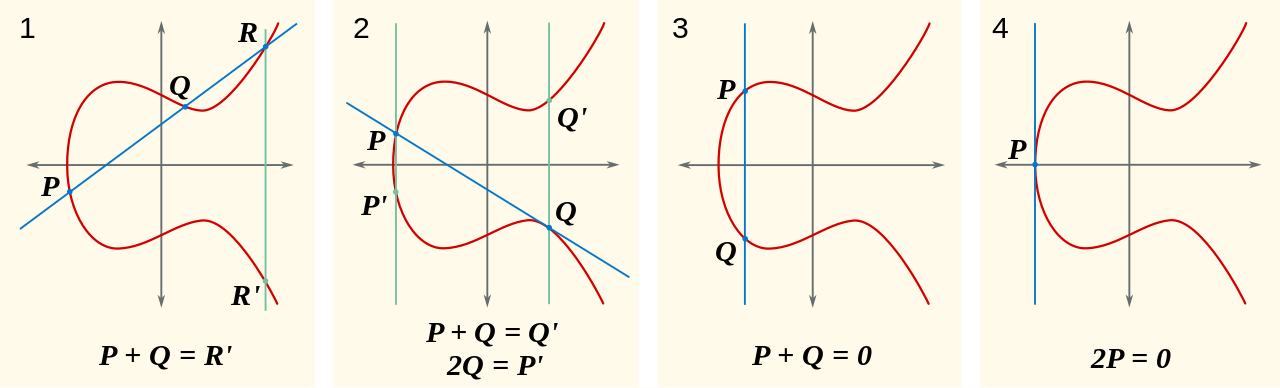
\includegraphics{assets/images/elliptic-curve-examples.png}
  \caption{Elliptic curve examples. Graphic cc-by-sa Emmanuel Boutet.}
  \label{fig:elliptic-curve-examples}
\end{figure}

Bitcoin basiert auf unserem besten Verständnis der Realität. Während es in der
Physik, Informatik und Mathematik noch viele offene Probleme gibt, sind wir uns
bei einigen Dingen ziemlich sicher. Dass es eine Asymmetrie zwischen dem Finden
von Lösungen und der Validierung der Richtigkeit dieser Lösungen gibt, ist eine
solche. Dass die Berechnung Energie benötigt ist eine andere. Mit anderen
Worten: Eine Nadel in einem Heuhaufen zu finden ist schwieriger, als zu prüfen
ob das spitze Ding in der Hand tatsächlich eine Nadel ist oder nicht. Die Nadel
zu finden erfordert viel Arbeit.

Die Weite vom Raum der Bitcoinadressen ist wahrlich unbegreiflich. Die Anzahl
der privaten Schlüssel sogar noch mehr. Es ist faszinierend wie viel von unserer
modernen Welt auf die Unwahrscheinlichkeit hinausläuft, eine Nadel in einem
unergründlich großen Heuhaufen zu finden. Ich bin mir dieser Tatsache heute mehr
denn je bewusst.

\paragraph{Bitcoin lehrte mich, dass eine unglaubliche Stärke in Zahlen steckt.}

% ---
%
% #### Down the Rabbit Hole
%
% - [How secure is 256 bit security?]["How secure is 256 bit security?"] by 3Blue1Brown
% - [Block Hashing Algorithm][hash functions] on the Bitcoin Wiki
% - [Last Glacial Maximum][thick layer of ice], [SHA-2][SHA-256], [Dyson Sphere][Dyson sphere], [Landauer's Principle][flip bits perfectly] [P versus NP][P actually equals NP], [Discrete Logarithm][specific problems] on Wikipedia
%
% [thick layer of ice]: https://en.wikipedia.org/wiki/Last_Glacial_Maximum
% [xkcd \#1125]: https://xkcd.com/1225/
% [SHA-256]: https://en.wikipedia.org/wiki/SHA-2
% [hash functions]: https://en.bitcoin.it/wiki/Block_hashing_algorithm
% ["How secure is 256 bit security?"]: https://www.youtube.com/watch?v=S9JGmA5_unY
% [Bruce Schneier]: https://www.schneier.com/
% [flip bits perfectly]: https://en.wikipedia.org/wiki/Landauer%27s_principle#Equation
% [Dyson sphere]: https://en.wikipedia.org/wiki/Dyson_sphere
% [2]: https://books.google.com/books?id=Ok0nDwAAQBAJ&pg=PT316&dq=%22These+numbers+have+nothing+to+do+with+the+technology+of+the+devices;%22&hl=en&sa=X&ved=0ahUKEwjXttWl8YLhAhUphOAKHZZOCcsQ6AEIKjAA#v=onepage&q&f=false
% [wrench attack]: https://xkcd.com/538/
% [call to cryptographic arms]: https://cryptome.org/2012/12/assange-crypto-arms.htm
% [P actually equals NP]: https://en.wikipedia.org/wiki/P_versus_NP_problem#P_=_NP
% [specific problems]: https://en.wikipedia.org/wiki/Discrete_logarithm#Cryptography
% [3Blue1Brown]: https://twitter.com/3blue1brown
%
% <!-- Wikipedia -->
% [alice]: https://en.wikipedia.org/wiki/Alice%27s_Adventures_in_Wonderland
% [carroll]: https://en.wikipedia.org/wiki/Lewis_Carroll

% \chapter{Reflections on ``Don't Trust, Verify''}
\label{les:16}

\begin{chapquote}{Lewis Carroll, \textit{Alice in Wonderland}}
``Now for the evidence,'' said the King, ``and then the sentence.''
\end{chapquote}

Bitcoin aims to replace, or at least provide an alternative to,
conventional currency. Conventional currency is bound to a centralized
authority, no matter if we are talking about legal tender like the US
dollar or modern monopoly money like Fortnite's V-Bucks. In both
examples, you are bound to trust the central authority to issue, manage
and circulate your money. Bitcoin unties this bound, and the main issue
Bitcoin solves is the issue of \textit{trust}.

\begin{samepage}\begin{quotation}
\enquote{The root problem with conventional currency is all the trust that's
required to make it work. [...] What is needed is an electronic
payment system based on cryptographic proof instead of trust}
\flushright -- Satoshi Nakamoto\footnote{Satoshi Nakamoto, official Bitcoin announcement~\cite{bitcoin-announcement} and whitepaper~\cite{whitepaper}}
\end{quotation}\end{samepage}

Bitcoin solves the problem of trust by being completely decentralized,
with no central server or trusted parties. Not even trusted \textit{third}
parties, but trusted parties, period. When there is no central
authority, there simply \textit{is} no-one to trust. Complete decentralization
is the innovation. It is the root of Bitcoin's resilience, the reason
why it is still alive. Decentralization is also why we have mining,
nodes, hardware wallets, and yes, the blockchain. The only thing you
have to \enquote{trust} is that our understanding of mathematics and physics
isn't totally off and that the majority of miners act honestly (which
they are incentivized to do).

While the regular world operates under the assumption of \textit{\enquote{trust,
but verify,}} Bitcoin operates under the assumption of \textit{\enquote{don't
trust, verify.}} Satoshi made the importance of removing trust very clear in
both the introduction as well as the conclusion of the Bitcoin whitepaper.

\begin{samepage}\begin{quotation}
\enquote{Conclusion: We have proposed a system for electronic transactions
without relying on trust.}
\flushright -- Satoshi Nakamoto\footnote{Satoshi Nakamoto, the Bitcoin whitepaper~\cite{whitepaper}}
\end{quotation}\end{samepage}

Note that \textit{without relying on trust} is used in a very specific context
here. We are talking about trusted third parties, i.e. other entities
which you trust to produce, hold, and process your money. It is assumed,
for example, that you can trust your computer.

As Ken Thompson showed in his Turing Award lecture, trust is an
extremely tricky thing in the computational world. When running a
program, you have to trust all kinds of software (and hardware) which,
in theory, could alter the program you are trying to run in a malicious
way. As Thompson summarized in his \textit{Reflections on Trusting Trust}:
\enquote{The moral is obvious. You can't trust code that you did not totally
create yourself.}~\cite{trusting-trust}

\begin{figure}
  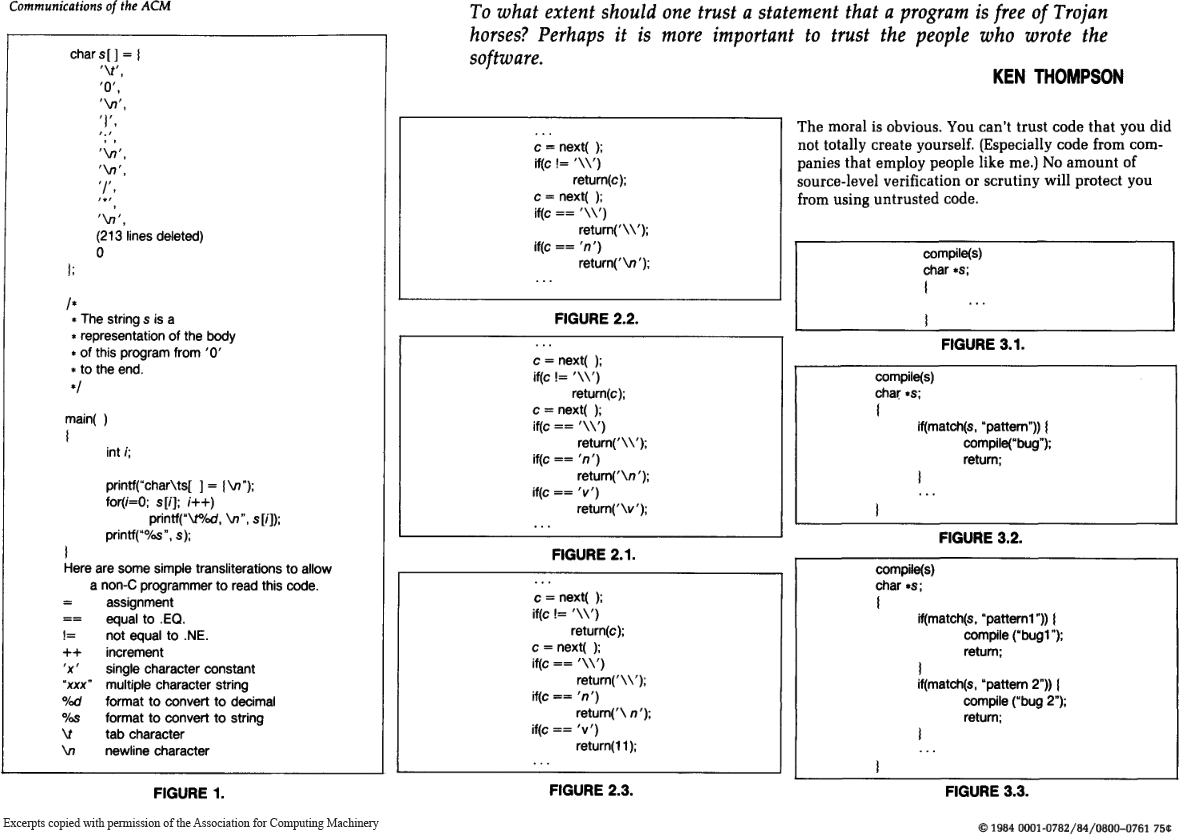
\includegraphics{assets/images/ken-thompson-hack.png}
  \caption{Excerpts from Ken Thompson's paper `Reflections on Trusting Trust'}
  \label{fig:ken-thompson-hack}
\end{figure}

Thompson demonstrated that even if you have access to the source code,
your compiler --- or any other program-handling program or
hardware --- could be compromised and detecting this backdoor would be
very difficult. Thus, in practice, a truly \textit{trustless} system does not
exist. You would have to create all your software \textit{and} all your
hardware (assemblers, compilers, linkers, etc.) from scratch, without
the aid of any external software or software-aided machinery.

\begin{samepage}\begin{quotation}
\enquote{If you wish to make an apple pie from scratch, you must first invent
the universe.}
\flushright -- Carl Sagan\footnote{Carl Sagan, \textit{Cosmos} \cite{cosmos}}
\end{quotation}\end{samepage}

The Ken Thompson Hack is a particularly ingenious and hard-to-detect backdoor,
so let's take a quick look at a hard-to-detect backdoor which works without
modifying any software. Researchers found a way to compromise security-critical
hardware by altering the polarity of silicon
impurities.~\cite{becker2013stealthy} Just by changing the physical properties
of the stuff that computer chips are made of they were able to compromise a
cryptographically secure random number generator. Since this change can't be
seen, the backdoor can't be detected by optical inspection, which is one of the
most important tamper-detection mechanism for chips like these.

\begin{figure}
  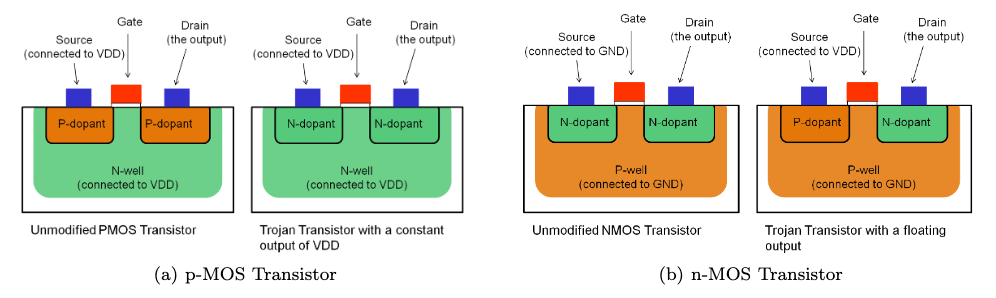
\includegraphics{assets/images/stealthy-hardware-trojan.png}
  \caption{Stealthy Dopant-Level Hardware Trojans by Becker, Regazzoni, Paar, Burleson}
  \label{fig:stealthy-hardware-trojan}
\end{figure}

Sounds scary? Well, even if you would be able to build everything from
scratch, you would still have to trust the underlying mathematics. You
would have to trust that \textit{secp256k1} is an elliptic curve without
backdoors. Yes, malicious backdoors can be inserted in the mathematical
foundations of cryptographic functions and arguably this has already
happened at least once.~\cite{wiki:Dual_EC_DRBG} There are good reasons to be paranoid, and the
fact that everything from your hardware, to your software, to the
elliptic curves used can have backdoors~\cite{wiki:backdoors} are some of them.

\begin{samepage}\begin{quotation}
``Don't trust. Verify.''
\flushright -- Bitcoiners everywhere
\end{quotation}\end{samepage}

The above examples should illustrate that \textit{trustless} computing is
utopic. Bitcoin is probably the one system which comes closest to this
utopia, but still, it is \textit{trust-minimized} --- aiming to remove trust
wherever possible. Arguably, the chain-of-trust is neverending, since
you will also have to trust that computation requires energy, that P
does not equal NP, and that you are actually in base reality and not
emprisoned in a simulation by malicious actors.

Developers are working on tools and procedures to minimize any remaining trust
even further. For example, Bitcoin developers created
Gitian\footnote{\url{https://gitian.org/}}, which is a software distribution
method to create deterministic builds. The idea is that if multiple developers
are able to reproduce identical binaries, the chance of malicious tampering is
reduced. Fancy backdoors aren't the only attack vector. Simple blackmail or
extortion are real threats as well. As in the main protocol, decentralization is
used to minimize trust.

Various efforts are being made to improve upon the chicken-and-egg problem of
bootstrapping which Ken Thompson's hack so brilliantly pointed
out~\cite{web:bootstrapping}. One such effort is
Guix\footnote{\url{https://guix.gnu.org}} (pronounced \textit{geeks}), which
uses functionally declared package management leading to bit-for-bit
reproducible builds by design. The result is that you don't have to trust any
software-providing servers anymore since you can verify that the served binary
was not tampered with by rebuilding it from scratch. Recently, a
pull-request was merged to integrate Guix into the Bitcoin build process.\footnote{See PR 15277 of \texttt{bitcoin-core}: \\ \url{https://github.com/bitcoin/bitcoin/pull/15277}}

\begin{figure}
  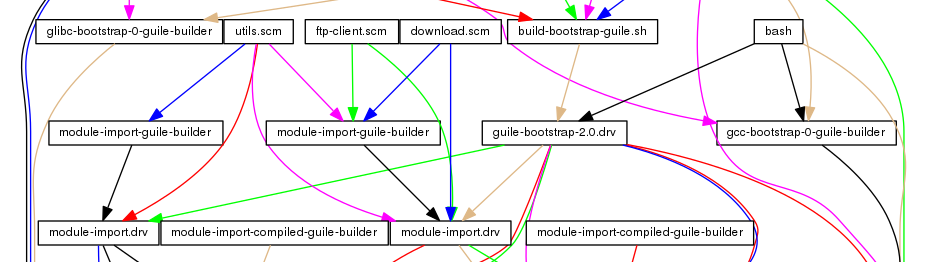
\includegraphics{assets/images/guix-bootstrap-dependencies.png}
  \caption{Which came first, the chicken or the egg?}
  \label{fig:guix-bootstrap-dependencies}
\end{figure}

Luckily, Bitcoin doesn't rely on a single algorithm or piece of
hardware. One effect of Bitcoin's radical decentralization is a
distributed security model. Although the backdoors described above are
not to be taken lightly, it is unlikely that every software wallet,
every hardware wallet, every cryptographic library, every node
implementation, and every compiler of every language is compromised.
Possible, but highly unlikely.

Note that you can generate a private key without relying on any computational
hardware or software. You can flip a coin~\cite{antonopoulos2014mastering} a
couple of times, although depending on your coin and tossing style this source
of randomness might not be sufficiently random. There is a reason why storage
protocols like Glacier\footnote{\url{https://glacierprotocol.org/}} advise to
use casino-grade dice as one of two sources of entropy.

Bitcoin forced me to reflect on what trusting nobody actually entails.
It raised my awareness of the bootstrapping problem, and the implicit
chain-of-trust in developing and running software. It also raised my
awareness of the many ways in which software and hardware can be
compromised.

\paragraph{Bitcoin taught me not to trust, but to verify.}

% ---
%
% #### Down the Rabbit Hole
%
% - [The Bitcoin whitepaper][Nakamoto] by Satoshi Nakamoto
% - [Reflections on Trusting Trust][\textit{Reflections on Trusting Trust}] by Ken Thompson
% - [51% Attack][majority] on the Bitcoin Developer Guide
% - [Bootstrapping][bootstrapping], Guix Manual
% - [Secp256k1][secp256k1] on the Bitcoin Wiki
% - [ECC Backdoors][backdoors], [Dual EC DRBG][has already happened] on Wikipedia
%
% [Emmanuel Boutet]: https://commons.wikimedia.org/wiki/User:Emmanuel.boutet
% [\textit{Reflections on Trusting Trust}]: https://www.archive.ece.cmu.edu/~ganger/712.fall02/papers/p761-thompson.pdf
% [found a way]: https://scholar.google.com/scholar?hl=en&as_sdt=0%2C5&q=Stealthy+Dopant-Level+Hardware+Trojans&btnG=
% [Gitian]: https://gitian.org/
% [bootstrapping]: https://www.gnu.org/software/guix/manual/en/html_node/Bootstrapping.html
% [Guix]: https://www.gnu.org/software/guix/
% [pull-request]: https://github.com/bitcoin/bitcoin/pull/15277
% [flip a coin]: https://github.com/bitcoinbook/bitcoinbook/blob/develop/ch04.asciidoc#private-keys
% [Glacier]: https://glacierprotocol.org/
% [secp256k1]: https://en.bitcoin.it/wiki/Secp256k1
% [majority]: https://bitcoin.org/en/developer-guide#term-51-attack
%
% <!-- Wikipedia -->
% [backdoors]: https://en.wikipedia.org/wiki/Elliptic-curve_cryptography#Backdoors
% [has already happened]: https://en.wikipedia.org/wiki/Dual_EC_DRBG
% [Carl Sagan]: https://en.wikipedia.org/wiki/Cosmos_%28Carl_Sagan_book%29
% [alice]: https://en.wikipedia.org/wiki/Alice%27s_Adventures_in_Wonderland
% [carroll]: https://en.wikipedia.org/wiki/Lewis_Carroll

% \chapter{Die Zeit zu bestimmen erfordert Arbeit}
\label{les:17}

\begin{chapquote}{Lewis Carroll, \textit{Alice im Wunderland}}
\enquote{Ach herrje! Ich werde zu spät kommen!}
\end{chapquote}

Es wird oft gesagt, dass Bitcoins \enquote{geschürft} werden weil tausende von
Computern an der Lösung \textit{sehr komplexer} mathematischer Probleme
arbeiten. Probleme wollen gelöst werden, und wenn man die richtige Antwort
berechnet hat, \enquote{produziert} man einen Bitcoin. Diese vereinfachte
Ansicht des Bitcoin-Minings ist zwar leichter zu verstehen, verfehlt aber den
Sinn etwas. Bitcoins werden nicht produziert oder erschaffen - und es geht nicht
darum mathematische Probleme zu lösen (zudem sind die Probleme nicht
mathematisch komplex). Es geht darum ein anderes Problem zu lösen: die
\textit{Bestimmung der Zeit} in einem dezentralen System.

Wie im Whitepaper beschrieben ist das Proof-of-Work-System (auch bekannt als
Mining) eine Möglichkeit, einen verteilten Zeitstempelserver zu implementieren.

\begin{center}
  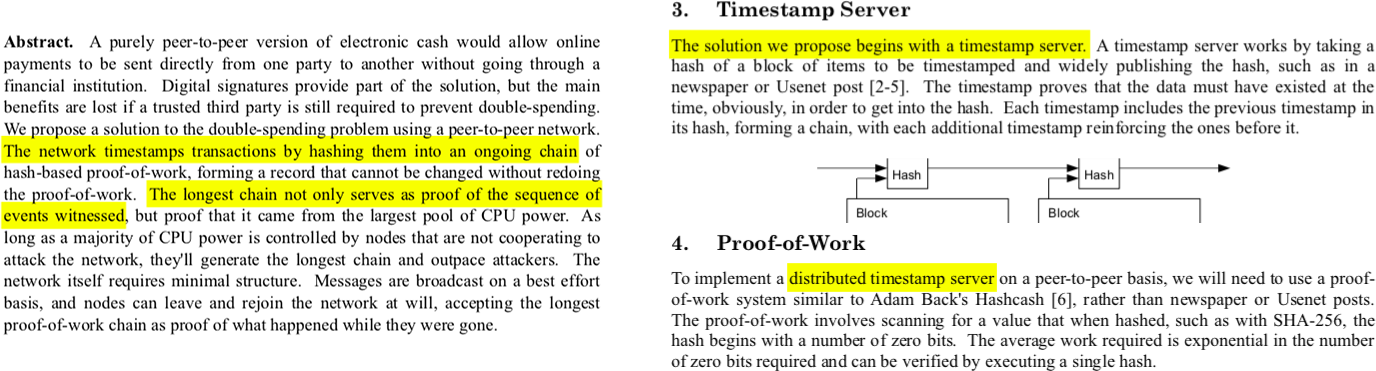
\includegraphics[width=\textwidth]{assets/images/bitcoin-whitepaper-timestamp-wide.png}
  \caption{Auszüge aus dem Bitcoin-Whitepaper}
  \label{fig:bitcoin-whitepaper-timestamp-wide}
\end{center}

Als ich lernte wie Bitcoin funktioniert dachte auch ich, dass Proof-of-Work
ineffizient und verschwenderisch sei. Nach einer Weile begann ich jedoch meine
Sichtweise auf den Energieverbrauch von Bitcoin zu ändern~\cite{gigi:energy}. Es
scheint, dass Proof-of-Work auch heute noch --- im Jahr 10 n.B. (nach Bitcoin)
--- weitestgehend missverstanden wird.

Da die Probleme, die beim Proof-of-Work zu lösen sind, frei erfunden werden
glauben viele Menschen, dass es \textit{sinnlose} Arbeit ist. Wenn der Fokus nur
auf der Berechnung liegt, ist dies eine verständliche Schlussfolgerung. Aber bei
Bitcoin geht es nicht um die Berechnung. Es geht darum sich \textit{unabhängig
über die Ordnung der Dinge zu einigen}.

Proof-of-Work ist ein System in dem jeder überprüfen kann was passiert ist und
in welcher Reihenfolge es passiert ist. Diese unabhängige Validierung führt zu
einem Konsens, zu einer individuellen Vereinbarung mehrerer Parteien darüber,
wer was besitzt.

In einer radikal dezentralen Umgebung haben wir nicht den Luxus einer absoluten
Zeit. Jede Uhr würde eine dritte Partei einführen der man vertrauen müsste --
ein zentraler Punkt im System auf den man sich verlassen muss und der
angegriffen werden kann. \enquote{Das Timing ist das eigentliche Problem}, wie
Grisha Trubetskoy betont~\cite{pow-clock}. Und Satoshi hat dieses Problem durch
die Implementierung einer dezentralen Uhr über eine Proof-of-Work-Blockchain
hervorragend gelöst. Alle sind sich im Voraus einig, dass die Kette mit der
meisten kumulierten Arbeit, die Quelle der Wahrheit ist. Es ist per Definition
das, was tatsächlich passiert ist. Dieses Abkommen ist das, was heute als
Nakamoto-Konsens bezeichnet wird.

\begin{quotation}\begin{samepage}
\enquote{Die Netzwerk-Zeitstempel kennzeichnen Transaktionen, indem sie in eine
fortlaufende Kette eingeordnet werden die als Beweis für die Abfolge der
beobachteten Ereignisse dient.}
\begin{flushright} -- Satoshi Nakamoto\footnote{Satoshi Nakamoto, Bitcoin Whitepaper~\cite{whitepaper}}
\end{flushright}\end{samepage}\end{quotation}

Ohne einen konsistenten Weg die Zeit zu definieren kann man kein
\enquote{vorher} und \enquote{nacher} definieren. Eine zuverlässige Ordnung ist
unmöglich. Wie bereits oben erwähnt, ist der Nakamoto-Konsens Bitcoins Art und
Weise die Zeit zu bestimmen. Die Anreizstruktur des Systems erzeugt eine
wahrscheinlichkeitsbezogene und dezentrale Uhr, indem sie sowohl die Gier als
auch das Eigeninteresse konkurrierender Teilnehmer nutzt. Die Tatsache, dass
diese Uhr ungenau ist, ist irrelevant da die Reihenfolge der Ereignisse
eindeutig ist und von jedem überprüft werden kann.

Dank Proof-of-Work sind sowohl die Arbeit, als auch die Validierung der
Arbeit radikal dezentralisiert. Jeder kann dem Netzwerk nach Belieben beitreten,
jeder kann das Netzwerk nach Belieben verlassen, und jeder kann alles jederzeit
überprüfen. Nicht nur das, jeder kann den Zustand des Systems
\textit{individuell} überprüfen ohne sich auf andere verlassen zu müssen.

Proof-of-Work zu verstehen erfordert Zeit. Es ist oft kontraintuitiv und obwohl
die Regeln einfach sind führen sie zu recht komplexen Phänomenen. Mir hat es
geholfen meine Sichtweise auf das Mining zu ändern. Nützlich, nicht nutzlos.
Validierung, nicht Berechnung. Zeit, nicht Blöcke.

\paragraph{Bitcoin lehrte mich, dass es schwierig ist die Zeit zu bestimmen,
besonders in dezentralen Systemen.}

% ---
%
% #### Through the Looking-Glass
%
% - [Bitcoin's Energy Consumption: A shift in perspective][energy]
%
% #### Down the Rabbit Hole
%
% - [Blockchain Proof-of-Work Is a Decentralized Clock][points out] by Gregory Trubetskoy
% - [The Anatomy of Proof-of-Work][pow-anatomy] by Hugo Nguyen
% - [PoW is efficient][pow-efficient] by Dan Held
% - [Mining][bw-mining], [Controlled supply][bw-supply] on the Bitcoin Wiki
%
% [points out]: https://grisha.org/blog/2018/01/23/explaining-proof-of-work/
% [energy]: 
% [whitepaper]: https://bitcoin.org/bitcoin.pdf
%
% [pow-efficient]: https://blog.picks.co/pow-is-efficient-aa3d442754d3
% [pow-anatomy]: https://bitcointechtalk.com/the-anatomy-of-proof-of-work-98c85b6f6667
% [bw-mining]: https://en.bitcoin.it/wiki/Mining
% [bw-supply]: https://en.bitcoin.it/wiki/Controlled_supply
%
% <!-- Wikipedia -->
% [alice]: https://en.wikipedia.org/wiki/Alice%27s_Adventures_in_Wonderland
% [carroll]: https://en.wikipedia.org/wiki/Lewis_Carroll

% ---
layout: lesson
title: Lesson 18
subtitle: Move slowly and don't break things
quote: "So the boat wound slowly along, beneath the bright summer-day, with its merry crew and its music of voices and laughter..."
categories: [bitcoin, lesson]
audio: /assets/audio/21lessons/3-18.m4a 
---

It might be a dead mantra, but "move fast and break things" is still how
much of the tech world operates. The idea that it doesn't matter if you
get things right the first time is a basic pillar of the *fail early,
fail often* mentality. Success is measured in growth, so as long as you
are growing everything is fine. If something doesn't work at first you
simply pivot and iterate. In other words: throw enough shit against the
wall and see what sticks.

Bitcoin is very different. It is different by design. It is different
out of necessity. As Satoshi [pointed out], e-currency has been tried
many times before, and all previous attempts have failed because there
was a head which could be cut off. The novelty of Bitcoin is that it is
a beast without heads.

> "A lot of people automatically dismiss e-currency as a lost cause
> because of all the companies that failed since the 1990's. I hope it's
> obvious it was only the centrally controlled nature of those systems
> that doomed them."
> <cite>[Satoshi Nakamoto][pointed out]</cite>

One consequence of this radical decentralization is an inherent
resistance to change. "Move fast and break things" does not and will
never work on the Bitcoin base layer. Even if it would be desirable, it
wouldn't be possible without convincing *everyone* to change their ways.
That's distributed consensus. That's the nature of Bitcoin.

> "The nature of Bitcoin is such that once version 0.1 was released, the
> core design was set in stone for the rest of its lifetime."
> <cite>[Satoshi Nakamoto][4]</cite>

This is one of the many paradoxical properties of Bitcoin. We all came
to believe that anything which is software can be changed easily. But
the nature of the beast makes changing it bloody hard.

As Hasu beautifully shows in [Unpacking Bitcoin's Social Contract],
changing the rules of Bitcoin is only possible by *proposing* a change,
and consequently *convincing* all users of Bitcoin to adopt this change.
This makes Bitcoin very resilient to change, even though it is software.

This resilience is one of the most important properties of Bitcoin.
Critical software systems have to be antifragile, which is what the
interplay of Bitcoin's social layer and its technical layer guarantees.
Monetary systems are adversarial by nature, and as we have known for
thousands of years solid foundations are essential in an adversarial
environment.

> "The rain came down, the floods came, and the winds blew, and beat on
> that house; and it didn't fall, for it was founded on the rock."
> <cite>[Matthew 7:24--27]</cite>

Arguably, in this parable of the wise and the foolish builders Bitcoin
isn't the house. It is the rock. Unchangeable, unmoving, providing the
foundation for a new financial system.

Just like geologists, who know that rock formations are always moving
and evolving, one can see that Bitcoin is always moving and evolving as
well. You just have to know where to look and how to look at it.

The introduction of [pay to script hash] and [segregated witness] are
proof that Bitcoin's rules can be changed if enough users are convinced
that adopting said change is to the benefit of the network. The latter
enabled the development of the [lightning network], which is one of the
houses being built on Bitcoin's solid foundation. Future upgrades like
[Schnorr signatures] will enhance efficiency and privacy, as well as
scripts (read: smart contracts) which will be indistinguishable from
regular transactions thanks to [Taproot]. Wise builders do indeed build
on solid foundations.

Satoshi wasn't only a wise builder technologically. He also understood
that it would be necessary to make wise decisions ideologically.

> "Being open source means anyone can independently review the code. If
> it was closed source, nobody could verify the security. I think it's
> essential for a program of this nature to be open source."
> <cite>[Satoshi Nakamoto][5]</cite>

Openness is paramount to security and inherent in open source and the
free software movement. As Satoshi pointed out, secure protocols and the
code which implements them have to be open --- there is no security
through obscurity. Another benefit is again related to decentralization:
code which can be run, studied, modified, copied, and distributed freely
ensures that it is spread far and wide.

The radically decentralized nature of Bitcoin is what makes it move
slowly and deliberately. A network of nodes, each run by a sovereign
individual, is inherently resistant to change --- malicious or not. With
no way to force updates upon users the only way to introduce changes is
by slowly convincing each and every one of those individuals to adopt a
change. This non-central process of introducing and deploying changes is
what makes the network incredibly resilient to malicious changes. It is
also what makes fixing broken things more difficult than in a
centralized environment, which is why everyone tries not to break things
in the first place.

Bitcoin taught me that moving slowly is one of its features, not a bug.

---

#### Through the Looking-Glass

- [Lesson 1: Immutability and Change][lesson1]

#### Down the Rabbit Hole

- [Unpacking Bitcoin's Social Contract] by Hasu
- [Schnorr signatures BIP][Schnorr signatures] by Pieter Wuille
- [Taproot proposal][Taproot] by Gregory Maxwell
- [P2SH][pay to script hash], [SegWit][segregated witness] on the Bitcoin Wiki
- [Parable of the Wise and the Foolish Builders][Matthew 7:24--27] on Wikipedia

<!-- Down the Rabbit Hole -->
[lesson1]: {{ '/bitcoin/lessons/ch1-01-immutability-and-change' | absolute_url }}

[pointed out]: http://p2pfoundation.ning.com/forum/topics/bitcoin-open-source?commentId=2003008%3AComment%3A9493
[4]: https://bitcointalk.org/index.php?topic=195.msg1611#msg1611
[Unpacking Bitcoin's Social Contract]: https://uncommoncore.co/unpacking-bitcoins-social-contract/
[Matthew 7:24--27]: https://en.wikipedia.org/wiki/Parable_of_the_Wise_and_the_Foolish_Builders
[pay to script hash]: https://en.bitcoin.it/wiki/Pay_to_script_hash
[segregated witness]: https://en.bitcoin.it/wiki/Segregated_Witness
[lightning network]: https://lightning.network/
[Schnorr signatures]: https://github.com/sipa/bips/blob/bip-schnorr/bip-schnorr.mediawiki#cite_ref-6-0
[Taproot]: https://lists.linuxfoundation.org/pipermail/bitcoin-dev/2018-January/015614.html
[5]: https://bitcointalk.org/index.php?topic=13.msg46#msg46

<!-- Wikipedia -->
[alice]: https://en.wikipedia.org/wiki/Alice%27s_Adventures_in_Wonderland
[carroll]: https://en.wikipedia.org/wiki/Lewis_Carroll

% \chapter{ Privacy is not Dead}
\label{les:19}

\begin{chapquote}{Lewis Carroll, \textit{Alice in Wonderland}}
The players all played at once without waiting for turns, and quarrelled all
the while at the tops of their voices, and in a very few minutes the Queen was
in a furious passion, and went stamping about and shouting ``off with his
head!'' of ``off with her head!'' about once in a minute.
\end{chapquote}

If pundits are to believed, privacy has been dead [since the 80ies]. The
pseudonymous invention of Bitcoin and other events in recent history
show that this is not the case. Privacy is alive, even though it is by
no means easy to escape the surveillance state.

Satoshi went through great lengths to cover up his tracks and conceal
his identity. Ten years later, it is still unknown if Satoshi Nakamoto
was a single person, a group of people, male, female, or a
[time-traveling AI] which bootstrapped itself to take over the world.
Conspiracy theories aside, Satoshi chose to identify himself to be a
Japanese male, which is why I don't assume but respect his chosen gender
and refer to him as *he*.

\begin{figure}
  
\includegraphics{assets/images/nope.png}
  \caption{I am not Dorian Nakamoto.}
  \label{fig:nope}
\end{figure}

Whatever his real identity might be, Satoshi was successful in hiding
it. He set an encouraging example for everyone who wishes to remain
anonymous: it is possible to have privacy online.

\begin{quotation}
``Encryption works. Properly implemented strong crypto systems are one
of the few things that you can rely on.''
\end{quotation}
% > <cite>[Edward Snowden]</cite>

Satoshi wasn't the first pseudonymous or anonymous inventor, and he
won't be the last. Some have directly imitated this pseudonymous
publication style, like Tom Elvis Yedusor of [MimbleWimble] fame, while
others have published advanced mathematical proofs while remaining
completely [anonymous].

It is a strange new world we are living in. A world where identity is
optional, contributions are accepted based on merit, and people can
collaborate and transact freely. It will take some adjustment to get
comfortable with these new paradigms, but I strongly believe that all of
this has the potential to change the world for the better.

We should all remember that privacy is a [fundamental human right]. And
as long as people exercise and defend these rights the battle for
privacy is far from over. Bitcoin taught me that privacy is not dead.

% ---
%
% #### Down the Rabbit Hole
%
% - [Universal Declaration of Human Rights][fundamental human right] by the United Nations
% - [A lower bound on the length of the shortest superpattern][anonymous] by Anonymous 4chan Poster, Robin Houston, Jay Pantone, and Vince Vatter
%
% [since the 80ies]: https://books.google.com/ngrams/graph?content=privacy+is+dead&year_start=1970&year_end=2019&corpus=15&smoothing=3&share=&direct_url=t1%3B%2Cprivacy%20is%20dead%3B%2Cc0
% [time-traveling AI]: https://blockchain24-7.com/is-crypto-creator-a-time-travelling-ai/
% ["I am not Dorian Nakamoto."]: http://p2pfoundation.ning.com/forum/topics/bitcoin-open-source?commentId=2003008%3AComment%3A52186
% [Edward Snowden]: https://www.theguardian.com/world/2013/jun/17/edward-snowden-nsa-files-whistleblower
% [MimbleWimble]: https://github.com/mimblewimble/docs/wiki/MimbleWimble-Origin
% [anonymous]: https://oeis.org/A180632/a180632.pdf
% [fundamental human right]: http://www.un.org/en/universal-declaration-human-rights/
%
% <!-- Wikipedia -->
% [alice]: https://en.wikipedia.org/wiki/Alice%27s_Adventures_in_Wonderland
% [carroll]: https://en.wikipedia.org/wiki/Lewis_Carroll

% \chapter{Cypherpunks Write Code}
\label{les:20}

\begin{chapquote}{Lewis Carroll, \textit{Alice in Wonderland}}
\enquote{I see you're trying to invent something.}
\end{chapquote}

Like many great ideas, Bitcoin didn't come out of nowhere. It was made
possible by utilizing and combining many innovations and discoveries in
mathematics, physics, computer science, and other fields. While
undoubtedly a genius, Satoshi wouldn't have been able to invent Bitcoin
without the giants on whose shoulders he was standing on.

\begin{quotation}\begin{samepage}
\enquote{He who only wishes and hopes does not interfere actively with the
course of events and with the shaping of his own destiny.}
\flushright -- Ludwig von Mises\footnote{Ludwig von Mises, \textit{Human Action} \cite{human-action}}
\end{samepage}\end{quotation}
% > <cite>[Ludwig Von Mises]</cite>

One of these giants is Eric Hughes, one of the founders of the cypherpunk
movement and author of \textit{A Cypherpunk's Manifesto}. It's hard to imagine
that Satoshi wasn't influenced by this manifesto. It speaks of many things which
Bitcoin enables and utilizes, such as direct and private transactions,
electronic money and cash, anonymous systems, and defending privacy with
cryptography and digital signatures.

\begin{quotation}\begin{samepage}
\enquote{Privacy is necessary for an open society in the electronic age.
[...] Since we desire privacy, we must ensure that each party to a
transaction have knowledge only of that which is directly necessary
for that transaction. [...]
Therefore, privacy in an open society requires anonymous transaction
systems. Until now, cash has been the primary such system. An
anonymous transaction system is not a secret transaction system.
[...]
We the Cypherpunks are dedicated to building anonymous systems. We are
defending our privacy with cryptography, with anonymous mail
forwarding systems, with digital signatures, and with electronic
money.
Cypherpunks write code.}
\flushright -- Eric Hughes\footnote{Eric Hughes, A Cypherpunk's Manifesto \cite{cypherpunk-manifesto}}
\end{samepage}\end{quotation}

Cypherpunks do not find comfort in hopes and wishes. They actively
interfere with the course of events and shape their own destiny.
Cypherpunks write code.

Thus, in true cypherpunk fashion, Satoshi sat down and started to write
code. Code which took an abstract idea and proved to the world that it
actually worked. Code which planted the seed of a new economic reality.
Thanks to this code, everyone can verify that this novel system actually
works, and every 10 minutes or so Bitcoin proofs to the world that it is
still living.

\begin{figure}
  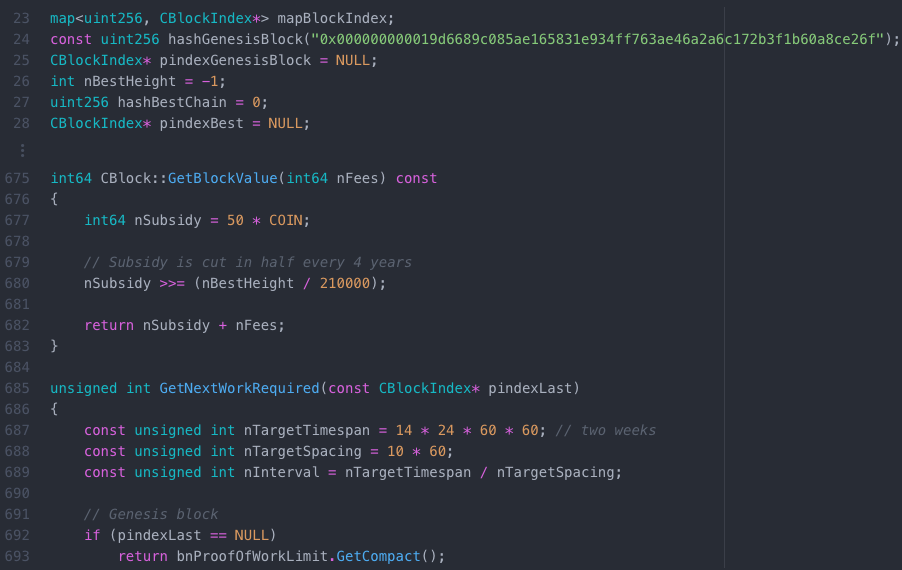
\includegraphics{assets/images/bitcoin-code.png}
  \caption{Code excerpts from Bitcoin version 0.1}
  \label{fig:bitcoin-code}
\end{figure}

To make sure that his innovation transcends fantasy and becomes reality, Satoshi
wrote code to implement his idea before he wrote the whitepaper. He also made
sure not to delay\footnote{\enquote{We shouldn't delay forever until every possible
feature is done.} -- Satoshi Nakamoto~\cite{satoshi-delay}} any release forever.
After all, \enquote{there's always going to be one more thing to do.}

\begin{quotation}\begin{samepage}
\enquote{I had to write all the code before I could convince myself that I
could solve every problem, then I wrote the paper.}
\flushright -- Satoshi Nakamoto\footnote{Satoshi Nakamoto, Re: Bitcoin P2P e-cash paper \cite{satoshi-mail-code-first}}
\end{samepage}\end{quotation}

In today's world of endless promises and doubtful execution, an exercise
in dedicated building was desperately needed. Be deliberate, convince
yourself that you can actually solve the problems, and implement the
solutions. We should all aim to be a bit more cypherpunk.

\paragraph{Bitcoin taught me that cypherpunks write code.}

% ---
%
% #### Down the Rabbit Hole
%
% - [Bitcoin version 0.1.0 announcement][version 0.1.0] by Satoshi Nakamoto
% - [Bitcoin P2P e-cash paper announcement][mail-announcement] by Satoshi Nakamoto
%
% [mail-announcement]: http://www.metzdowd.com/pipermail/cryptography/2008-October/014810.html
% [Ludwig Von Mises]: https://mises.org/library/human-action-0/html/pp/613
% [version 0.1.0]: https://bitcointalk.org/index.php?topic=68121.0
% [not to delay]: https://bitcointalk.org/index.php?topic=199.msg1670#msg1670
% [6]: http://www.metzdowd.com/pipermail/cryptography/2008-November/014832.html
%
% <!-- Wikipedia -->
% [alice]: https://en.wikipedia.org/wiki/Alice%27s_Adventures_in_Wonderland
% [carroll]: https://en.wikipedia.org/wiki/Lewis_Carroll

% \chapter{ Metaphors for Bitcoin's Future}
\label{les:21}

\begin{chapquote}{Lewis Carroll, \textit{Alice in Wonderland}}
``I know something interesting is sure to happen...''
\end{chapquote}

In the last couple of decades, it became apparent that technological
innovation does not follow a linear trend. Whether you believe in the
technological singularity or not, it is undeniable that progress is
exponential in many fields. Not only that, but the rate at which
technologies are being adopted is accelerating, and before you know it
the bush in the local schoolyard is gone and your kids are using
Snapchat instead. Exponential curves have the tendency to slap you in
the face way before you see them coming.

Bitcoin is an exponential technology built upon exponential
technologies. [Our World in Data] beautifully shows [the rising speed of
technological adoption], starting in 1903 with the introduction of
landlines. Landlines, electricity, computers, the internet, smartphones;
all follow exponential trends in price-performance and adoption. Bitcoin
does too.

% 

Bitcoin has not one but [multiple network effects], all of which
resulting in exponential growth patterns in their respective area:
price, users, security, developers, market share, and adoption as global
money.

Having survived its infancy, Bitcoin is continuing to grow every day in
more aspects than one. Granted, the technology has not reached maturity
yet. It might be in its adolescence. But if the technology is
exponential, the path from obscurity to ubiquity is short.

% 

In his 2003 [TED talk], Jeff Bezos chose to use electricity as a
metaphor for the web's future. All three phenomena --- electricity, the
internet, Bitcoin --- are *enabling* technologies, networks which enable
other things. They are infrastructure to be built upon, foundational in
nature.

Electricity has been around for a while now. We take it for granted. The
internet is quite a bit younger, but most people already take it for
granted as well. Bitcoin is ten years old and has entered public
consciousness during the last hype cycle. Only the earliest of adopters
take it for granted. As [more time] passes, more and more people will
recognize Bitcoin as something which simply is.

In 1994, the internet was still confusing and unintuitive. Watching this
old [recording of the Today Show] makes it obvious that what feels
natural and intuitive now actually wasn't back then. Bitcoin is still
confusing and alien to most, but just like the internet is second nature
for digital natives, spending and [stacking] sats will be second nature
to the bitcoin natives of the future.

\begin{quotation}
``The future is already here --- it's just not very evenly
distributed.''
\end{quotation}
% > <cite>[William Gibson]</cite>

In 1995, about 15% of American adults used the internet. Historical
[data from the Pew Research Center] shows how the internet has woven
itself into all our lives. According to a [consumer survey] by Kaspersky
Lab, 13\% of respondents have used Bitcoin and its clones to pay for
goods in 2018. While payments aren't the only use-case of bitcoin, it is
some indication of where we are in Internet time: in the early- to
mid-90s.

In 1997, Jeff Bezos stated in a [letter to shareholders] that "this is
Day 1 for the Internet," recognizing the great untapped potential for
the internet and, by extension, his company. Whatever day this is for
Bitcoin, the vast amounts of untapped potential are clear to all but the
most casual observer.

% 

Bitcoin's first node went online in 2009 after Satoshi mined the
[genesis block] and released the software into the wild. His node wasn't
alone for long. Hal Finney was one of the first people to pick up on the
idea and join the network. Ten years later, as of this writing, more
than
[75.000](https://luke.dashjr.org/programs/bitcoin/files/charts/software.html)
nodes are [running bitcoin].

The protocol's base layer isn't the only thing growing exponentially.
The lightning network, a second layer technology, is growing at an even
faster rate.

In January 2018, the lightning network had [40 nodes] and 60 channels.
In April 2019, the network grew to more than 4000 nodes and around
40.000 channels. Keep in mind that this is still experimental technology
where loss of funds can and does occur. Yet the [trend is clear][Jameson Lopp]:
thousands of people are [reckless] and eager to use it.

% 

To me, having lived through the meteoric rise of the web, the parallels
between the internet and Bitcoin are obvious. Both are networks, both
are exponential technologies, and both enable new possibilities, new
industries, new ways of life. Just like electricity was the best
metaphor to understand where the internet is heading, the internet might
be the best metaphor to understand where bitcoin is heading. Or, in the
words of Andreas Antonopoulos, Bitcoin is [*The Internet of Money*].
These metaphors are a great reminder that while history doesn't repeat
itself, it often rhymes.

Exponential technologies are hard to grasp and often underestimated.
Even though I have a great interest in such technologies, I am
constantly surprised by the pace of progress and innovation. Watching
the Bitcoin ecosystem grow is like watching the rise of the internet in
fast-forward. It is exhilarating.

My quest of trying to make sense of Bitcoin has led me down the pathways
of history in more ways than one. Understanding ancient societal
structures, past monies, and how communication networks evolved were all
part of the journey. From the handaxe to the smartphone, technology has
undoubtedly changed our world many times over. Networked technologies
are especially transformational: writing, roads, electricity, the
internet. All of them changed the world. Bitcoin has changed mine and
will continue to change the minds and hearts of those who dare to use
it.

Bitcoin taught me that understanding the past is essential to
understanding its future. A future which is just beginning.

% ---
%
% #### Down the Rabbit Hole
%
% - [The Rising Speed of Technological Adoption][the rising speed of technological adoption] by Jeff Desjardins
% - [The 7 Network Effects of Bitcoin][multiple network effects] by Trace Mayer
% - [The Electricity Metaphor for the Web's Future][TED talk] by Jeff Bezos
% - [How the internet has woven itself into American life][data from the Pew Research Center] by Susannah Fox and Lee Rainie
% - [Genesis Block][genesis block] on the Bitcoin Wiki
% - [Lindy Effect][more time] on Wikipedia
%
% [Our World in Data]: https://ourworldindata.org/
% [the rising speed of technological adoption]: https://www.visualcapitalist.com/rising-speed-technological-adoption/
% [multiple network effects]: https://www.thrivenotes.com/the-7-network-effects-of-bitcoin/
% [TED talk]: https://www.ted.com/talks/jeff_bezos_on_the_next_web_innovation
% [recording of the Today Show]: https://www.youtube.com/watch?v=UlJku_CSyNg
% [William Gibson]: https://www.npr.org/2018/10/22/1067220/the-science-in-science-fiction
% [data from the Pew Research Center]: https://www.pewinternet.org/2014/02/27/part-1-how-the-internet-has-woven-itself-into-american-life/
% [consumer survey]: https://www.kaspersky.com/blog/money-report-2018/
% [letter to shareholders]: http://media.corporate-ir.net/media_files/irol/97/97664/reports/Shareholderletter97.pdf
% [running bitcoin]: https://twitter.com/halfin/status/1110302988?lang=en
% [40 nodes]: https://bitcoinist.com/bitcoin-lightning-network-mainnet-nodes/
% [reckless]: https://twitter.com/hashtag/reckless
% [Jameson Lopp]: https://twitter.com/lopp/status/1077200836072296449
% [*The Internet of Money*]: https://theinternetofmoney.info/
% [stacking]: https://twitter.com/hashtag/stackingsats
%
% <!-- Bitcoin Wiki -->
% [genesis block]: https://en.bitcoin.it/wiki/Genesis_block
%
% <!-- Wikipedia -->
% [more time]: https://en.wikipedia.org/wiki/Lindy_effect
% [alice]: https://en.wikipedia.org/wiki/Alice%27s_Adventures_in_Wonderland
% [carroll]: https://en.wikipedia.org/wiki/Lewis_Carroll

% \addpart{Final Thoughts}
\pdfbookmark{Conclusion}{conclusion}
\label{ch:conclusion}

\chapter*{Conclusion}

\begin{chapquote}{Lewis Carroll, \textit{Alice im Wunderland}}
\enquote{Begin at the beginning} the King said, very gravely, \enquote{and go on till you
come to the end: then stop.}
\end{chapquote}

As mentioned in the beginning, I think that any answer to the
question \textit{“What have you learned from Bitcoin?”} will always be incomplete. The
symbiosis of what can be seen as multiple living systems -- Bitcoin, the
technosphere, and economics -- is too intertwined, the topics too numerous, and
things are moving too fast to ever be fully understood by a single person.

Even without understanding it fully, and even with all its quirks and seeming
shortcomings, Bitcoin undoubtedly works. It keeps producing blocks roughly every
ten minutes and does so beautifully. The longer Bitcoin continues to work, the
more people will opt-in to use it.

\begin{quotation}\begin{samepage}
\enquote{It's true that things are beautiful when they work. Art is function.}
\begin{flushright} -- Giannina Braschi\footnote{Giannina Braschi, \textit{Empire of Dreams} \cite{braschi2011empire}}
\end{flushright}\end{samepage}\end{quotation}

\paragraph{} Bitcoin is a child of the internet. It is growing exponentially,
blurring the lines between disciplines. It isn’t clear, for example, where the
realm of pure technology ends and where another realm begins. Even though
Bitcoin requires computers to function efficiently, computer science is not
sufficient to understand it. Bitcoin is not only borderless in regards to its
inner workings but also boundaryless in respect to academic disciplines.

Economics, politics, game theory, monetary history, network theory, finance,
cryptography, information theory, censorship, law and regulation, human
organization, psychology -- all these and more are areas of expertise which might
help in the quest of understanding how Bitcoin works and what Bitcoin is.

No single invention is responsible for its success. It is the combination of
multiple, previously unrelated pieces, glued together by game theoretical
incentives, which make up the revolution that is Bitcoin. The beautiful blend of
many disciplines is what makes Satoshi a genius.

\paragraph{} Like every complex system, Bitcoin has to make tradeoffs in terms
of efficiency, cost, security, and many other properties. Just like there is no
perfect solution to deriving a square from a circle, any solution to the
problems which Bitcoin tries to solve will always be imperfect as well.

\begin{quotation}\begin{samepage}
\enquote{I don’t believe we shall ever have a good money again before we take the
thing out of the hands of government, that is, we can’t take it violently
out of the hands of government, all we can do is by some sly roundabout way
introduce something that they can’t stop.}
\begin{flushright} -- Friedrich Hayek\footnote{Friedrich Hayek on Monetary Policy, the Gold Standard, Deficits, Inflation, and John Maynard Keynes \url{https://youtu.be/EYhEDxFwFRU}}
\end{flushright}\end{samepage}\end{quotation}

Bitcoin is the sly, roundabout way to re-introduce good money to the world. It
does so by placing a sovereign individual behind each node, just like Da Vinci
tried to solve the intractable problem of squaring a circle by placing the
Vitruvian Man in its center. Nodes effectively remove any concept of a center,
creating a system which is astonishingly antifragile and extremely hard to shut
down. Bitcoin lives, and its heartbeat will probably outlast all of ours.

I hope you have enjoyed these twenty-one lessons. Maybe the most important
lesson is that Bitcoin should be examined holistically, from multiple angles, if
one would like to have something approximating a complete picture. Just like
removing one part from a complex system destroys the whole, examining parts of
Bitcoin in isolation seems to taint the understanding of it. If only one person
strikes \enquote{blockchain} from her vocabulary and replaces it with \enquote{a
chain of blocks} I will die a happy man.

In any case, my journey continues. I plan to venture further down into the
depths of this rabbit hole, and I invite you to tag
along for the ride.\footnote{\url{https://twitter.com/dergigi}}

% <!-- Twitter -->
% [dergigi]: https://twitter.com/dergigi
%
% <!-- Internal -->
% [sly roundabout way]: https://youtu.be/EYhEDxFwFRU?t=1124
% [Giannina Braschi]: https://en.wikipedia.org/wiki/Braschi%27s_Empire_of_Dreams


\bibliography{main}

\end{document}
